%%%%%%%%%%%%%%%%%%%%%%%%%%%%%%%%%%%%%%%%%%%%%%%%%%%%%%%%%%%%%%%%%%%%%%%%%%%%%%%%
%% JSS Header/Packages                                                        %%
%%                                                                            %%
%%                                                                            %%
%%%%%%%%%%%%%%%%%%%%%%%%%%%%%%%%%%%%%%%%%%%%%%%%%%%%%%%%%%%%%%%%%%%%%%%%%%%%%%%%
\documentclass[article]{jss}

\usepackage{amsmath, amssymb} 
\usepackage{orcidlink, thumbpdf, lmodern}
\usepackage{array} 
\usepackage{pdfpages} 
\usepackage{multirow} % for multirow
\newcommand{\class}[1]{`\code{#1}'}
\newcommand{\fct}[1]{\code{#1()}}
\newcommand{\mbf }[1]{\mbox{\boldmath ${#1}$}}

%%%%%%%%%%%%%%%%%%%%%%%%%%%%%%%%%%%%%%%%%%%%%%%%%%%%%%%%%%%%%%%%%%%%%%%%%%%%%%%%
%% Title, Author                                                              %%
%%                                                                            %%
%%                                                                            %%
%%%%%%%%%%%%%%%%%%%%%%%%%%%%%%%%%%%%%%%%%%%%%%%%%%%%%%%%%%%%%%%%%%%%%%%%%%%%%%%%
%% -- Article metainformation (author, title, ...) -----------------------------
%% - \author{} with primary affiliation
%% - \Plainauthor{} without affiliations
%% - Separate authors by \And or \AND (in \author) or by comma (in \Plainauthor).
%% - \AND starts a new line, \And does not.
\author{Bo-Syue Jiang\\National Taipei University
\And Han-Ming Wu~\orcidlink{0000-0001-9464-3127}\\National Chengchi University}
\Plainauthor{Bo-Syue Jiang, Han-Ming Wu}

%% - \title{} in title case
%% - \Plaintitle{} without LaTeX markup (if any)
%% - \Shorttitle{} with LaTeX markup (if any), used as running title
\title{\pkg{ggESDA}: An \proglang{R} Package for Exploratory \\ Symbolic Data Analysis using \pkg{ggplot2}}
\Plaintitle{ggESDA: An R Package for Exploratory Symbolic Data Analysis based on ggplot2}
\Shorttitle{ggESDA package in \proglang{R}}

%%%%%%%%%%%%%%%%%%%%%%%%%%%%%%%%%%%%%%%%%%%%%%%%%%%%%%%%%%%%%%%%%%%%%%%%%%%%%%%%
%% Abstract, Keywords                                                         %%
%%                                                                            %%
%%                                                                            %%
%%%%%%%%%%%%%%%%%%%%%%%%%%%%%%%%%%%%%%%%%%%%%%%%%%%%%%%%%%%%%%%%%%%%%%%%%%%%%%%%
\Abstract{
Exploratory data analysis (EDA) serves as a preliminary yet essential
tool for summarizing the main characteristics of a data set before
appropriate statistical modeling can be applied. Quite often, EDA
employs the traditional graphical techniques such as the boxplot,
histogram and scatterplot and are equipped with various dimension
reduction methods and computer-aided interactive functionalities. EDA
has been used to explore different data types. Examples were the cases
of the survival data, the time series data, the functional data and
the longitudinal data. Conventionally, these data set were tabulated
by a table with $p$ columns corresponding to $p$ variables. Each
subject is measured by a single numerical value for each variable.
Nowadays the collected data keeps getting bigger and complex. The
description of data was no longer stored by a form of a single value
but the intervals, histograms and/or distributions. These are examples
of the so-called symbolic data. This study develops an \proglang{R}
package, namely \pkg{ggESDA}, as an extension of \pkg{ggplot2} package
for exploring symbolic data through a wide variety of plots. SDA
supplies various data descriptions and has great capacity for large
and complex data. The \pkg{ggESDA} acts as an advanced graphical tool
that supports the efficient, effective and practical exploration of
symbolic data sets.
}

%% - \Keywords{} with LaTeX markup, at least one required
%% - \Plainkeywords{} without LaTeX markup (if necessary)
%% - Should be comma-separated and in sentence case.
\Keywords{data visualization, exploratory data analysis, interval-valued data, statistical graphics, symbolic data analysis}
\Plainkeywords{data visualization, exploratory data analysis, interval-valued data, statistical graphics, symbolic data analysis}

%%%%%%%%%%%%%%%%%%%%%%%%%%%%%%%%%%%%%%%%%%%%%%%%%%%%%%%%%%%%%%%%%%%%%%%%%%%%%%%%
%% Address, Affiliations                                                      %%
%%                                                                            %%
%%                                                                            %%
%%%%%%%%%%%%%%%%%%%%%%%%%%%%%%%%%%%%%%%%%%%%%%%%%%%%%%%%%%%%%%%%%%%%%%%%%%%%%%%%
%% - \Address{} of at least one author
%% - May contain multiple affiliations for each author
%%   (in extra lines, separated by \emph{and}\\).
%% - May contain multiple authors for the same affiliation
%%   (in the same first line, separated by comma).
\Address{
  Wu, Han-Ming\\
  Faculty of Department of Statistics\\
  National Chengchi University\\
  No. 64, Sec. 2, ZhiNan Rd., Wenshan District, \\
  Taipei City 11605, Taiwan\\
  E-mail: \email{wuhm@g.nccu.edu.tw}\\
  URL: \url{http://www.hmwu.idv.tw}
}


\begin{document}
%%%%%%%%%%%%%%%%%%%%%%%%%%%%%%%%%%%%%%%%%%%%%%%%%%%%%%%%%%%%%%%%%%%%%%%%%%%%%%%%
%% Introduction                                                               %%
%%                                                                            %%
%%                                                                            %%
%%%%%%%%%%%%%%%%%%%%%%%%%%%%%%%%%%%%%%%%%%%%%%%%%%%%%%%%%%%%%%%%%%%%%%%%%%%%%%%%
%% - In principle "as usual".
%% - But should typically have some discussion of both _software_ and _methods_.
%% - Use \proglang{}, \pkg{}, \fct{}, \code{} markup throughout the manuscript.
%% - If such markup is in (sub)section titles, a plain text version has to be
%%   added as well.
%% - All software mentioned should be properly \cite-d.
%% - All abbreviations should be introduced.
%% - Unless the expansions of abbreviations are proper names (like "Journal
%%   of Statistical Software" above) they should be in sentence case (like
%%   "generalized linear models" below).
\section[Introduction]{Introduction} \label{sec:intro}

%% SDA
For the conventional data analysis, the data set were usually
presented by a classical data table where $p$ random variables are
represented by a single point in $p$-dimensional space. In contrast,
symbolic data with measurements on $p$ random variables are
$p$-dimensional statistical units such as hypercubes or histograms in
$\mathbb{R}^p$, or a Cartesian product of $p$ distributions. The
symbolic data analysis (SDA) was proposed by Billard and Diday (2003,
2007). The aim is to provide an overview of the statistical
methodologies for analyzing such data. Symbolic variables make
possible to describe groups of individuals and concepts. In practice,
the symbolic data is generated by aggregating the large or enormous
datasets into intervals or histograms. The aggregation can produce a
dataset of more manageable size in order to conduct appropriate
analyses; or it can originate to some scientific questions of
interest. These are very important characteristics of SDA so that it
could be served as a potential solution for big data problem. The
researches for interval-valued data such as the sign test for COVID-19
data \cite{sherwani:2021}, the prediction via regularized artificial
neural network \cite{yang:2019}, a bivariate Bayesian method for
regression models \cite{xu:2021}, etc. Figure \ref{fig:trend} shows
the number of the SDA related researches including clustering,
classification, forecasting and so on is increasing among year 1998 to
2020 based on several database, which outstands the importance of it
during the years. Among ScienceDirect, Engineering and Computer
Science lead the subject areas obviously, shown in Figure
\ref{fig:subjectAreas}.

%% EDA
Exploratory data analysis (EDA) was pioneered by Tukey (1977). The
main goal of EDA is to obtain a general sense of the data by mostly
employing a variety of graphical techniques such as scatterplots,
boxplots and histograms. Quite often, the dimension reduction methods
are also used to visualize multivariate data. There are some
advantages of graphical approaches to data analysis over the
traditional formal statistical modeling and inference, including (1)
summaries for large, complicated data sets; (2) checking assumptions
in statistical models; (3) interaction between the researcher and the
data; (4) revealing structure, patterns, features, trends, anomalies,
and relationships in data; (5) communicating the results of an
analysis; (6) identifying the areas of interest. EDA is especially
useful in early stages of data mining. Due to the popularity of data
science and big data, EDA regains people's attention in the recent
years for pattern discovery and statistical visualization.

%% why EDA for SD
The typical graphical techniques used in EDA such as the index plot,
boxplot, scatter plot and histogram were developed for the classical
data can not be applied directly to various symbolic data types such
as interval-valued data, histogram-valued data, distribution-valued
data and so on. On the other hand, when the dimensionality of symbolic
data is high, one way to explore the insight structure of symbolic
objects in the lower-dimensional space is to employ the DR methods. As
a consequence, the development of an EDA tool with more visual methods
and the advanced DR techniques for symbolic data is needed.

%% R Packages, ggESDA
The \proglang{R} packages benefit users to analyze their data without
difficulties. There have several \proglang{R} packages that related to
the symbolic data analysis (see Table \ref{tab:sda_packages}). The
contexts include the formal statistical modeling and inference.
However, little work has been conducted on the exploratory analysis
and visualization. This motivates us to develop an \proglang{R}
package, namely \pkg{ggESDA}, aiming at exploring symbolic data
graphically. \pkg{ggESDA} is composed of the features to deal with the
interval-valued data, statistics data frame, clustering results, and
other components from \pkg{R6} \cite{R6} class. The graphical
techniques for interval-valued data can be divided into three
categories: univariate, bivariate, and multivariate. \pkg{ggESDA} is
designed to provides an overview of symbolic data sets and obtains a
general understanding about the variables and their relationships.


%% Article structure
This article is structured as follows. Section \ref{sec:design}
introduces the \pkg{ggESDA} package design and features with some
descriptive statistics for symbolic data. Section \ref{sec:graphics}
describes the implementation of plots for exploring the real world
interval-valued data. Principal component analysis (PCA) for
interval-valued data with other functionalities are given in Section
\ref{sec:pca} and \ref{sec:others}. We then conclude with our results
in Section \ref{sec:conclusion}.


%%%%%%%%%%%%%%%%%%%%%%%%%%%%%%%%%%%%%%%%%%%%%%%%%%%%%%%%%%%%%%%%%%%%%%%%%%%%%%%%
%% ggESDA                                                                     %%
%%                                                                            %%
%%                                                                            %%
%%%%%%%%%%%%%%%%%%%%%%%%%%%%%%%%%%%%%%%%%%%%%%%%%%%%%%%%%%%%%%%%%%%%%%%%%%%%%%%%
%% -- Manuscript ---------------------------------------------------------------

%% - In principle "as usual" again.
%% - When using equations (e.g., {equation}, {eqnarray}, {align}, etc.
%%   avoid empty lines before and after the equation (which would signal a new
%%   paragraph.
%% - When describing longer chunks of code that are _not_ meant for execution
%%   (e.g., a function synopsis or list of arguments), the environment {Code}
%%   is recommended. Alternatively, a plain {verbatim} can also be used.
%%   (For executed code see the next section.)
%\section{Models and software} \label{sec:models}
\section{The SDA-related packages and the ggESDA package design}\label{sec:design}


%%%%%%%%%%%%%%%%%%%%%%%%%%%%%%%%%%%%%%%%%%%%%%%%%%%%%%%%%%%
%                                                         %
%                                                         %
%%%%%%%%%%%%%%%%%%%%%%%%%%%%%%%%%%%%%%%%%%%%%%%%%%%%%%%%%%%
\subsection{The SDA-related Packages}
There have several \proglang{R} packages that related to
the symbolic data analysis (see Table \ref{tab:sda_packages}). The
contexts include the formal statistical modeling and inference.
However, little work has been conducted on the exploratory analysis
and visualization. This motivates us to develop an \proglang{R}

The most prominent packages on CRAN are commonly used for statistical
or machine learning analyze. It can be briefly classified into two
parts, one is focused on statistic analysis, and the other is general
SDA packages including both analysis method and some graphical
technology. Nevertheless, most of their graphical technology tends to
use the basic graphics in \proglang{R} rather than \pkg{ggplot2}, or
only visualizes univariate distribution which is difficult to present
the relationship between variables.

Exploratory data analysis is cross-classified in two different ways
where each method is either graphical or non-graphical. And then, each
method is either univariate, bivariate or multivariate. \pkg{ggESDA}
uses a high-level graphic system by \pkg{ggplot2} \cite{ggplot2} to solve the problem
mentioned above and provides a variety of EDA methods in all kinds of
the variate.


\pkg{ggESDA} is a \proglang{R} data visualization library based on \pkg{ggplot2}. It provides
a high-level interface for drawing attractive and informative
statistical graphics.


In \proglang{Python}, we can also find the SDA package such as
\pkg{iardacil} \cite{umbleja:2020} which is available from the Github
at \url{https://github.com/iardacil/SDA}. The zoomstart software in
\pkg{iardacil} is provided with SODAS software project
\cite{diday:2008}. It is a basic thinking for general radar plot,
improved for distinct groups visualization by \pkg{ggESDA}, and
implemented in \proglang{R} using \pkg{ggplot2}.
 
%%%%%%%%%%%%%%%%%%%%%%%%%%%
% Table                   %
%%%%%%%%%%%%%%%%%%%%%%%%%%% Main Features
\begin{table}[t!]
\centering{\scriptsize
\begin{tabular}{|l|c|l|l|l|l} \hline
Package & Symbolic & Description & Plots &  Reference & Data Analysis Functionality \\
        & Object$^*$   &               &       &      &     \\
 \hline 
\pkg{RSDA}  & I & R to Symbolic Data Analysis
 & scatterplot, radar& Rojas {\it et al.} (2015) & GLM, Kmeans, Regression, PCA, KNN, Neural Networks, FA(factor analysis), RF, SVM, GBM\\
\pkg{symbolicDA} & I & Analysis of Symbolic Data
 & radar & Dudek {\it et al.} (2013)& Dynamical clustering, Decision Tree, HINoV,  pseudo F-statistic, Kernel, Discriminant analysis, Kohonen's self-organizing maps, PCA, RF \\
\pkg{HistDAWass} & H & Histogram-Valued Data Analysis & histogram, box, index& Irpino (2015) & Ramer-Douglas-Peucke, Moving average smoothing, KNN, Kurthosis, Quantile-Quantile correlation, Skewness, PCA, Multiple regression, K-means, Fuzzy c-means, Hierarchical clustering\\
\pkg{MAINT.Data} & I & Model and Analyse Interval Data
 & - & Silva \&  Brito (2011)&  LRT, Discriminant Analysis, MANOVA, Mixture model estimation, MLE \\
\pkg{iRegression} & I & Regression Methods for Interval-Valued Variables
 & - & Neto {\it et al.} (2011) & Regression, Bivariate regression \\
\pkg{intReg} & I & Interval Regression
 & - & Toomet (2012)  & Regression\\
\pkg{ISDA.R} & I & interval symbolic data analysis for R
 & histogram & Filho \&  Fagundes (2012) & Regression\\
\pkg{GPCSIV} & H & Generalized Principal Component of Symbolic Interval variables
 & - & Brahim (2013) & PCA\\
\pkg{GraphPCA} & H & Graphical Tools of Histogram PCA
 & - & Brahim \& Kallyth (2014) & PCA\\
\pkg{ggESDA} & I & Exploratory Symbolic Data Analysis with 'ggplot2' & index, scatter, radar, etc. & Jiang (2022) & PCA \\ \hline
\multicolumn{5}{l}{\footnotesize{$^*$I for the interval-valued objects, H for the histogram-valued objects.}}
\end{tabular}}%
\caption{\label{tab:sda_packages} The main features and the 
plots provided by the various \proglang{R} packages for symbolic data on CRAN.}
\end{table}%


%%%%%%%%%%%%%%%%%%%%%%%%%%%%%%%%%%%%%%%%%%%%%%%%%%%%%%%%%%%
%                                                         %
%                                                         %
%%%%%%%%%%%%%%%%%%%%%%%%%%%%%%%%%%%%%%%%%%%%%%%%%%%%%%%%%%%
\subsection{The ggESDA package designs}
"Exploratory Data Analysis is majorly performed using the following methods:
Univariate analysis:- provides summary statistics for each field in the raw data set (or) summary only on one variable. Ex:- CDF,PDF,Box plot, Violin plot.(don't worry, will see below what each of them is)
Bivariate analysis:- is performed to find the relationship between each variable in the dataset and the target variable of interest (or) using 2 variables and finding the relationship between them.Ex:-Box plot, Violin plot.
Multivariate analysis:- is performed to understand interactions between different fields in the dataset (or) finding interactions between variables more than 2. Ex:- Pair plot and 3D scatter plot."




%%%%%%%%%%%%%%%%%%%%
%                  %
%%%%%%%%%%%%%%%%%%%%
\subsubsection{Descriptive statistics}
The main content of EDA relates to the basic numerical summaries of
data (e.g., the central tendency measures, and variation or
variability measures) and the basic graphical summaries of data. For
example, the five-number summary of numerical data (minimum, 25\%
quartiles, median, 70\% quartiles, and maximum) is used to construct a
boxplot. Therefore, the basic descriptive statistics for symbolic data
should be provided prior to the (some) graphing techniques. In
addition, if we want to do the standardization or apply PCA to
interval-valued data, the mean, variance and the covariance must be
calculated first. There are many algorithms to calculate these
descriptive statistics for interval-valued data. For examples, the
methods we have introduced in Section \ref{ipca} of part were the
quantification methods, the quantile method, the distributional
methods, and the interval arithmetic methods. As a consequence,
choosing the appropriate methods to obtain the basic descriptive
statistics for symbolic data is the first step to implement the
exploratory symbolic data analysis.


The main content of EDA relates to the basic numerical summaries of
data (e.g., the central tendency measures, and variation or
variability measures) and the basic graphical summaries of data. For
example, the five-number summary of numerical data (minimum, $25\%$
quartiles, median, $70\%$ quartiles, and maximum) is used to construct
a boxplot. In the field of SDA, there are many algorithms to calculate
descriptive statistics and frequency for interval-valued data, and we
will illustrate the univariate and bivariate summaries respectively.


To build a statistic chart or analysis, descriptive statistics are
necessary to be constructed, as well as the frequency occurring in
each bin in a histogram chart. For a histogram chart, subdivisions of
it into equidistant and non-equidistant will also be consider in this
section.

For the quantile in interval-valued data, summarizing it may seem to
be obvious to separate data into a minimum and maximum data table,
then calculate quantiles of both data tables to build a new
interval-valued quantile data table.


%%%%%%%%%%%%%%%%%%%%%%%%%%%
% Table                   %
%%%%%%%%%%%%%%%%%%%%%%%%%%%
\begin{table}[t!]
\centering
\begin{tabular}{|l|l|} \hline
            & Statistics    \\ \hline
Univariate  & internal mean, grand mean, range, sd, variance, quantile  \\ \hline
Bivariate & covariance, correlation ($r, \rho, \tau$)\\ \hline
\end{tabular}
\caption{\label{tab:stat} The implemented summary statistics.}
\end{table}



%%%%%%%%%%%%%%%%%%%%
%                  %
%%%%%%%%%%%%%%%%%%%%
\subsubsection{Graphics design}
The typical graphical techniques of EDA include the index plot,
barplot, boxplot, and histogram for univariate data; the 2D
scatterplot, joint histogram and double boxplot for bivariate data;
and the satterplot matrix, and star plot for multivariate data. Of
course, there are many other variants of graphical techniques have
been proposed. Our aim in this study is to implement good statistical
graphics to display symbolic data accurately and clearly.

A good picture is worth a 1,000 words. The typical graphical
techniques of EDA include the index plot, barplot, boxplot, and
histogram for univariate data; the 2D scatterplot, joint histogram and
double boxplot for bivariate data; and the scatterplot matrix, and star
plot for multivariate data. Of course, there are many other variants
of graphical techniques have been proposed. Our aim in this study is
to implement the good statistical graphics to display symbolic data
accurately and clearly. On the other hand, it's worth mentioning that
there will be some advanced graphics implemented which are called the
min-max plot, and center-range plot due to the characteristics of
interval-valued data. 


The concept behind \pkg{ggplot2} consists of three different fundamental parts: 
\begin{quote}
{\tt Plot = data + Aesthetics + Geometry.}
\end{quote}
The principal components of every plot can be defined as follow:
\begin{enumerate}
\item data is a data frame.
\item Aesthetics is used to indicate $x$ and $y$ variables. It can also be used to control the color, the size or the shape of points, the height of bars, etc.
\item Geometry defines the type of graphics such as histogram, box plot, line plot, density plot, dot plot, and so on.
\end{enumerate}

General \pkg{ggplot2} syntax
\begin{verbatim}
ggplot(data, aes(...)) + geom() + ... + stat() + ...
\end{verbatim}

\begin{CodeChunk}
\begin{CodeInput}
R> library(ggplot2)
R> ggplot(data = iris, aes(x = Sepal.Length, y = Sepal.Width, color = Species)) +
         geom_point(size = 3)
\end{CodeInput}
\end{CodeChunk}

The package \pkg{ggESDA} is developed to as an extension of \pkg{ggplot2} to the interval-valued data. 
It provides a general and customized
transformation function \code{classic2sym} implemented for generating
a symbolic data table from classical data frame by clustering
algorithm using the \pkg{RSDA} package \cite{RSDA} form and
generalized \pkg{ggESDA} to other prominent SDA packages in
\proglang{R}.

General \pkg{ggESDA} syntax

\begin{verbatim}
ggInterval_<graphtype>(data = intervaldata, mapping = aes(...)) + geom() + ... + stat() + ...
\end{verbatim}

\begin{footnotesize}
The graphical types are shown in Table \ref{tab:graphics}.
\end{footnotesize}


%can delete : cannot use
%or
%\begin{verbatim}
%ggplot(data = intervaldata, mapping = aes(...)) + geom_I() + ... + stat_I() + ...
%\end{verbatim}

\begin{CodeChunk}
\begin{CodeInput}
R> library(ggESDA)
R> ggInterval_index(data = facedata, aes(x = AD, fill = IND)) +
         geom_point()
\end{CodeInput}
\end{CodeChunk}
%can delete
% #or
%R> ggplot(data = facedata, aes(x = AD, y = BC, color = IND)) +
%         geom_I_point()

Table \ref{tab:stat} lists the implemented summary statistics.
The implemented graphics are given in Table \ref{tab:graphics}.
All are based on the content of the books:
"Symbolic Data Analysis: Conceptual Statistics and Data Mining"
and
"Symbolic Data Analysis and the SODAS Software".


A possible source of interval data is the aggregation of a numerical
dataset. That is, the data is clustered into groups by some criterion
and the intervals are constructed by summarizing values into the
minimum value and maximum value within each group. One of the
advantage is that a large dataset can be summarized into a more
manageable size, the interval-valued symbolic data still retaining as
much knowledge inherent to the entire dataset as possible. The
aggregation of an object with data.frame class into an object of the
IntervalData class is by the function \fct{classic2sym()}.

The \pkg{ggESDA}
aims to convert the traditional data into the \pkg{ggESDA} object and
visualizes the symbolic data using \pkg{ggplot2}, which is shown in
Figure \ref{fig:pkgStr}. Each row (observation) in the conventional
data matrix $X_{p \times p}$ in the figure contains a vector of
numeric values, $O_i = (x_1,x_2,\cdots,x_n)$, while each row of the
interval-valued data matrix $I_{k \times p}$ contains a vector of
intervals (ranges), $C_j =
([a_{j1},b_{j1}],[a_{j2},b_{j2}],\cdots,[a_{jp},b_{jp}])$, called a
CONCEPT (or UNIT). The CONCEPT describe the behavior of a group of
observations. Thus, the aggregation method between them is an
essential process in SDA. See Section \ref{sec:aggregation} for details.



%%%%%%%%%%%%%%%%%%%%%%%%%%%
% Table                   %
%%%%%%%%%%%%%%%%%%%%%%%%%%%
\begin{table}[t!]
\centering
\begin{tabular}{|l|l|} \hline
Variate          & Graphics    \\ \hline
Univariate  & index plot, histogram, box plot, min-max plot, center-range plot \\ \hline
Bivariate & scatterplot, 2D-histogram \\ \hline
Multivariate & radar, scatterplot matrix, 2D-histogram matrix, image\\ \hline
\end{tabular}
\caption{\label{tab:graphics} The implemented graphics.}
\end{table}



%%%%%%%%%%%%%%%%%%%%
%                  %
%%%%%%%%%%%%%%%%%%%%
\subsubsection{Built-in datasets and object class}
In the following, we used the face recognition
data to illustrate some graphing functions we have implemented so far.

The face recognition data is widely used in the SDA literature (\cite{leroy:1996}; \cite{douzal:2011}; \cite{le:2012}). The dataset gives six face measurements of nine
men (Figure \ref{fig:face}), each with three observations, resulting in a
total 27 observations (Table \ref{facedata}). The measurements for
each observation came from a sequence of over 1,000 images. They cover
a range of values, hence interval-valued variables.


\begin{CodeChunk}
\begin{CodeInput}
R> library(ggESDA)
R> data(facedata)
R> facedata
\end{CodeInput}
\begin{CodeOutput}
                 AD              BC                AH
         <symblc_n>      <symblc_n>        <symblc_n>
1 [155.00 : 157.00] [58.00 : 61.01] [100.45 : 103.28]
2 [154.00 : 160.01] [57.00 : 64.00] [101.98 : 105.55]
3 [154.01 : 161.00] [57.00 : 63.00]  [99.36 : 105.65]
...
\end{CodeOutput}
\end{CodeChunk}




In the following, to illustrate some graphing functions we have implemented so far, we will use the two well-known symbolic datasets. One is face recognition data (\cite{leroy:1996}; \cite{douzal:2011}; \cite{le:2012}). The dataset gives six face measurements of nine men (Figure \ref{fig:face}), each with three observations, resulting in a total 27 observations. The measurements for each observation came from a sequence of over 1,000 images. They cover a range of values, hence interval-valued variables. 

The other is the Environment questionnaire data (from the SODAS software package \cite{diday:2008}). Because of the demonstration of the performance dealing with modal multi-valued data, the same datasets were used in the radar plot. This dataset contains 14 objects and 17 variables and 4 of them are modal multi-valued, while the rest are interval-valued variables. Both of the part of example datasets are shown as follow:


%%%%%%%%%%%%%%%%%%%%%%%%%%%
% Table                   %
%%%%%%%%%%%%%%%%%%%%%%%%%%%
\begin{table}[t!]
\centering {\scriptsize
\begin{tabular}{lll}\hline
  Data  & Reference& Usage \\
  \hline
  facedata & \cite{douzal:2011}; \cite{le:2012}& iPCA \\
  oils  & \cite{lauro2000principal}; \cite{lauro2008principal}& iPCA \\
  mushroom & \cite{neto2011bivariate}; \cite{domingues2010robust}& iRegression \\
  Cardiological (blood pressure) & \cite{billard2000regression}; \cite{xu2010symbolic}& iRegression \\
  AbaloneIdt & \cite{malerba2001comparing}& Dissimilarity measure \\
  Environment & \cite{umbleja:2020}& EDA \\
   \hline
\end{tabular}}
\caption{\label{tab:classic2sym} Summaries of the built-in interval-valued data.}
\end{table}%


%%%%%%%%%%%%%%%%%%%%%%%%%%%%%%%%%%%%%%%%%%%%%%%%%%%%%%%%%%%%%%%%%%%%%%%%%%%%%%%%
%% Descriptive statistics                                                     %%
%%                                                                            %%
%%                                                                            %%
%%%%%%%%%%%%%%%%%%%%%%%%%%%%%%%%%%%%%%%%%%%%%%%%%%%%%%%%%%%%%%%%%%%%%%%%%%%%%%%%
\section{Descriptive statistics for interval-valued data}

%%%%%%%%%%%%%%%%%%%%%%%%%%%%%%%%%%%%%%%%%%%%%%%%%%%%%%%%%%%
%                                                         %
%                                                         %
%%%%%%%%%%%%%%%%%%%%%%%%%%%%%%%%%%%%%%%%%%%%%%%%%%%%%%%%%%%
\subsection{Descriptive univariate statistics}
%% mean, median, mode, quantile
%% sd, variance
%% The empirical density function
%% frequency table

%%%%%%%%%%%%%%%%%%%%
%                  %
%%%%%%%%%%%%%%%%%%%%
\subsubsection{Quantification approaches}
In statistics, it may be more interesting to discuss mean and variance
in a particular random variable $Z$; see \cite{bertrand:2000}. The
realization of $Z$ for the observation $W_u$ is the interval $Z(W_u) =
[a_u,b_u]$, where $u=1,2,\cdots,m$ and $m$ is the number of concepts.




%%%%%%%%%%%%%%%%%%%%
%                  %
%%%%%%%%%%%%%%%%%%%%
\subsubsection{Distributional approaches}
First of all, assume that each object is equally likely to be observed with probability $\frac{1}{m}$, and the empirical density function of $Z$ is defined as : 

\begin{equation}\label{eq:dist1}
f(\xi) = \frac{1}{m} \sum_{u:\xi \in Z(W_u)}(\frac{1}{b_u-a_u})
\end{equation}

where $\xi$ is the individual descriptions.


The Equation (\ref{eq:dist1}) is also equivalently to :

\begin{equation}\label{eq:dist2}
f(\xi) = \frac{1}{m}\sum_{u \in E}\frac{I_u(\xi)}{\| Z(u) \|}\;,\xi \in \mathbb{R}
\end{equation}

where $I_u(.)$ is the indicator function that $\xi$ is or is not in the interval $Z(u)$, $\| Z(u) \|$ is the length of that interval, and $E=\{w_1,w_2,\cdots,w_m \}$.

Further, the symbolic sample mean from definition for $Z$ is $\bar{Z} = \int_{-\infty}^{\infty} \xi f(\xi)\;d\xi$, which can be reduced as :

\begin{equation}\label{eq:mean}
\bar{Z}=\frac{1}{m}\sum_{u \in E}\frac{a_u+b_u}{2}
\end{equation}

Finally, after getting the sample mean, the symbolic sample variance can be defined as follow:

\begin{equation}\label{eq:varDef}
\begin{split}
S^2 & = \int_{-\infty}^{\infty} (\xi - \bar{z})^2f(\xi)\;d\xi \\
 & = \int_{-\infty}^{\infty} \xi^2f(\xi)\;d\xi-\bar{z}
\end{split}
\end{equation}

and substituting for $f(\xi)$ from Equation (\ref{eq:dist2}), we have 
\begin{equation}\label{eq:derived}
\begin{split}
\int_{-\infty}^{\infty} \xi^2f(\xi)\;d\xi &= \frac{1}{m}\sum_{u \in E}\int_{-\infty}^{\infty} \xi^2 \frac{I_u(\xi)}{\| Z(u) \|}\;d\xi \\
&= \frac{1}{m}\sum_{u \in E} \int_{a_u}^{b_u} \frac{\xi^2}{(b_u-a_u)}\;d\xi \\
&= \frac{1}{3m} \sum_{u \in E}(\frac{b_u^3 - a_u^3}{b_u-a_u})
\end{split}
\end{equation}

Hence,
\begin{equation}\label{eq:var}
S^2 = \frac{1}{3m} \sum_{u \in E}(a_u^2+a_ub_u+b_u^2)-\frac{1}{4m^2}\left[ \sum_{u \in E}(a_u+b_u) \right]^2
\end{equation}



%%%%%%%%%%%%%%%%%%%%%%%%%%%%%%
%                            %
%%%%%%%%%%%%%%%%%%%%%%%%%%%%%%
\subsubsection{Frequency distribution tables}\label{sec:hist}
"The frequency distribution table reflects how often an occurrence has taken place in the data. It gives a brief idea of the data and makes it easier to find patterns."

For the univariate histogram frequency, assume that we partition the interval $I=[\min_{u \in E} a_u,\\ \max_{u \in E} b_u]$ into $r$ subintervals, and all of them in the histogram are equal distance. That is, $I_g = [\zeta_{g-1},\zeta_{g}),g=1,2,\cdots,r$, then $\| I_j \| = \| I_k \| , j,k=1,2,\cdots,r$. As a consequence, the observed frequency of the interval-valued variate $Z$ for the histogram subinterval $I_g$ from the definitions is

\begin{equation}\label{eq:fg}
f_g = \sum_{u \in E}\frac{\| Z(u) \cap I_g \|}{\| Z(u) \|}
\end{equation}

Moreover, for the interval-valued variate $Z$, we can pool the $a_u$ and $b_u$ from the interval of all observations, and sort it as a new vector $(x^{(1)},x^{(2)}, \cdots, x^{(2m)})$ to represent the cut of a histogram. The subinterval from the cut is then defined as $I'_g = [x^{(j)},x^{(j+1)})$, where $j = 1,2,\cdots, 2m-1$, and apply the Equation (\ref{eq:fg}) to get frequency. In most cases, $\| I'_g \|$ will not be equal to another, so we can get another histogram type, called non-equidistant-bin histogram.



%%%%%%%%%%%%%%%%%%%%%%%%%%%%%%
%                            %
%%%%%%%%%%%%%%%%%%%%%%%%%%%%%%
\subsubsection{Standardization of interval-valued data}
Before performing iSIR algorithm, we first standardize each
interval-valued variable of the data to have zero mean and unit
variance. This standardization prevents variables with
larger measurement scale from dominating those with
smaller scales. De Carvalho {\it et al.}, (2006) proposed
three standardization approaches for interval-valued
variables:  dispersion of the interval
centers, dispersion of the interval
boundaries, and the global range.

In this study, the general rule for standardizing
interval-valued variables $\Xi_j, j=1,\cdots, p$, consists in
performing the same transformation separately to both the lower
and upper bounds of all intervals $[a_{ij}, b_{ij}]$, which 
standardizes all point values between $a_{ij}$ and $b_{ij}$ 
in the same linear way
\[
\xi_{ij}^s = \left[\frac{a_{ij}-\bar{\xi}_j}{\varsigma_j},
 \frac{b_{ij}-\bar{\xi}_j}{\varsigma_j}\right],
\]
where $\bar{\xi}_{j}$ is the sample mean of interval
variable $\Xi_j$ given in Equation (\ref{xi.mean}) and
$\varsigma_j$ is the sample standard deviation of interval
variable $\Xi_j$. The sample standard deviation
$\varsigma_j$ is estimated following different iSIR
methods. With the exception of the distributional approaches, the general estimate of
$\varsigma_j$ is given by the standard deviation of the 
interval centers, i.e.,
\[
%\bar{\xi}_{j} = \frac{1}{n}\sum_{j=1}^n\frac{a_{ij}+b_{ij}}{2},\quad \mbox{and}\quad
 \varsigma_j=\left[\frac{1}{n}\sum_{i=1}^n\left(\frac{a_{ij}+b_{ij}}{2}-
\bar{\xi}_j\right)^2\right]^{1/2}.
\]
For EJD, GQ, and SPT,
$\varsigma_j$  
\textcolor{black}{is obtained from}
Equation (\ref{sj}). 


%%%%%%%%%%%%%%%%%%%%%%%%%%%%%%
%                            %
%%%%%%%%%%%%%%%%%%%%%%%%%%%%%%
\subsubsection{An example}


\begin{CodeChunk}
\begin{CodeInput}
R> mean(facedata)
\end{CodeInput}
\begin{CodeOutput}
	    AD    BC    AH    DH    EH    GH
	  <dbl> <dbl> <dbl> <dbl> <dbl> <dbl>
1  	163.  60.0  113.  113.  59.8  57.7
\end{CodeOutput}

\begin{CodeInput}
R> sd(facedata$AD)
\end{CodeInput}
\begin{CodeOutput}
[1] 6.816762
\end{CodeOutput}

%$
%%%%%%%%%%%%%%%%%%%%%%%%%%%%%%%%%%%%%%%%%%%%%%%%%%%%%%%%%%%
%                                                         %
%                                                         %
%%%%%%%%%%%%%%%%%%%%%%%%%%%%%%%%%%%%%%%%%%%%%%%%%%%%%%%%%%%
\subsection{Descriptive bivariate statistics}
%% covariance, correlation
%% joint density function



%%%%%%%%%%%%%%%%%%%%%%%%%%%%%%
%                            %
%%%%%%%%%%%%%%%%%%%%%%%%%%%%%%
\subsubsection{The empirical joint density method (EJD)}
For bivariates interval-valued variables, $Z_1$ and $Z_2$ , the 
observations on the rectangle 
$Z(u)= Z_1(u)\times Z_2(u) = ([a_{1u}, b_{1u}],
[a_{2u}, b_{2u}])$ for each $u \in E$. 
Assume individual vectors $x \in vir(d_u)$ are each uniformly distributed over 
the respective intervals $Z_1(u)$ and $Z_2(u)$.
%\item
%Therefore, the joint distribution of $(Z 1, Z_2)$ is a copula $C(z_1, z_2)$
Define the empirical joint density function for $(Z_1, Z_2)$:
\[ 
f(\xi_1, \xi_2)=
\frac{1}{m}\sum_{u \in E} \frac{I_u(\xi_1, \xi_2)}{\|Z(u)\|},
\]
where $I_u(\xi_1, \xi_2)$ is the indicator function that $(\xi_1, \xi_2)$ is or 
is not in the rectangle $Z(u)$ and where $\|Z(u)\|$ is the area of
this rectangle.  The bivariate interval-valued variables covariance function is 
defined as
\begin{eqnarray*}
cov(Z_1, Z_2)&=&  S_{Z_1 Z_2} =
\int_{-\infty}^{\infty}
(\xi_1 - \bar{Z_1})(\xi_2 -\bar{Z_2})f(\xi_1, \xi_2)\ d\xi_1 d\xi_2\\
&=&
\frac{1}{m} \sum_{u \in E}
\frac{1}{(b _{1u}-a_{1u})(b_{2u}-a_{2u})} \\
&&\times \iint_{(\xi_1, \xi_2)\in Z(u)}
\xi_1 \xi_2\ d\xi_1 d\xi_2 -\bar{Z_1}\bar{Z_2}\\
&=&
\frac{1}{4m}
\sum_{u \in E}(b_{1u}+ a_{1u})(b_{2u} + a_{2u}) \\
&&-\frac{1}{4m^2}\left[ \sum_{u \in E}
(b_{1u}+a_{1u})\right]\left[\sum_{u \in E}
(b_{2u}+a_{2u})\right].
\end{eqnarray*}


Many of the principles developed for the univariate case can be expanded to a general $p$-variate case, $p > 1$. We shall focus attention on obtaining joint histograms for $p = 2$. The following will reveal the statistics and bivariate histogram.

Linear Correlation

For bivariates interval-valued variables, $Z_1$ and $Z_2$, the observations $u$, where $u \in E$, on the rectangle $Z(u) = Z_1(u) \times Z_2(u)$ is $([a_{1u}, b_{1u}], [a_{2u}, b_{2u}])$. Assume the individual description vectors $\xi$ are each uniformly distributed over the respective intervals $Z_1(u)$ and $Z_2(u)$.  Define the empirical joint density function for $(Z_1, Z_2)$:

\begin{equation}\label{eq:bi_density}
f(\xi_1,\xi_2)=\frac{1}{m}\sum_{u \in E}\frac{I_u(\xi_1,\xi_2)}{\| Z(u) \|}
\end{equation}

where $I_u(\xi_1,\xi_2)$ is the indicator function that $(\xi_1,\xi_2)$ is or is not in the rectangle $Z_u$ and where $\|Z(u)\|$ is the area of this rectangle.

There is three methods to calculate bivariate interval-valued variables covariance function. For the first one, it can be derived by \cite{billard:2003} as following:

\begin{equation}\label{eq:cov}
cov(Z_1,Z_2)=\frac{1}{4m}\sum_{u \in E}(b_{1u} + a_{1u})(b_{2u} + a_{2u})-\frac{1}{4m^2}\left[ \sum_{u \in E}(b_{1u} + a_{1u}) \right]\left[ \sum_{u \in E}(b_{2u} + a_{2u}) \right]
\end{equation}




%%%%%%%%%%%%%%%%%%%%%%%%%%%%%%
%                            %
%%%%%%%%%%%%%%%%%%%%%%%%%%%%%%
\subsubsection{The symbolic covariance method (GQ)}
Second, an alternative expression of the symbolic sample variance for $Z$ in Equation (\ref{eq:var}) can be expressed as

\[
S^2 = \frac{1}{3m}\sum_{u \in E}\left[  (a_u-\bar{Z})^2 +(a_u-\bar{Z})(b_u-\bar{Z})+(b_u-\bar{Z})^2 \right]
\]

The above equation can be generalized by \cite{Billard+Diday:2007} to formulate the form of the symbolic sample covariance for $Z_j$ and $Z_{j\prime}$ as

\begin{equation}\label{eq:gq_cov}
cov(Z_j,Z_{j^{ \prime}}) = \frac{1}{3m}\sum_{i=1}^{m}G_jG_{j^{\prime}}\left[ Q_jQ_{j^\prime} \right]^{1/2}, \;\;j,j^\prime=1,2,\cdots,p
\end{equation}

where for $J = j,j^\prime$, 

\[
\begin{split}
Q_J &= (a_{iJ} - \bar{Z_J})^2 +(a_{iJ} - \bar{Z_J})(b_{iJ} - \bar{Z_J})+(b_{iJ} - \bar{Z_J})^2,\\
G_J &= \left\{\begin{array}{l}
          \begin{split}
          -1 &, \;\;\mbox{if} \;\; \xi_{iJ}^{c} \leq \bar{Z_J}\\
           1 &,  \;\;\mbox{if} \;\;  \xi_{iJ}^{c} > \bar{Z_J}
           \end{split}
        \end{array}\right.
\end{split}
\]

and $\xi_{iJ}^{c}$ is the midpoint of the interval $[a_{iJ},b_{iJ}]$.




%%%%%%%%%%%%%%%%%%%%%%%%%%%%%%
%                            %
%%%%%%%%%%%%%%%%%%%%%%%%%%%%%%
\subsubsection{The total sum of products (SPT)}
Last, it was further demonstrated by \cite{billard:2007} and \cite{billard:2008} that the sample variance in Equation (\ref{eq:var})
is a function of the total sum of squares (SST) and that the SST can be decomposed into the sum of the internal (within) variation and the between variation. The total sum of products (SPT) is the sum of the within sum of products and the between sum of products. The Equation (\ref{eq:var}) was also extended to the bivariate case to obtain the sample covariance of $Z_j$ and $Z_{j^\prime}$ based on the decomposition of the SPT as

\begin{equation}\label{eq:spt_cov}
%\begin{split}
cov(Z_j,Z_{j^{ \prime}}) = \frac{1}{6m}\sum_{i = 1}^m \left[ 2(a_{ij}-\bar{Z}_j)(a_{ij^\prime}-\bar{Z}_{j^\prime}) +(a_{ij}-\bar{Z}_j)(b_{ij^\prime}-\bar{Z}_{j^\prime})\\
+(b_{ij}-\bar{Z}_j)(a_{ij^\prime}-\bar{Z}_{j^\prime})+2(b_{ij}-\bar{Z}_j)(b_{ij^\prime}-\bar{Z}_{j^\prime})\right]
%\end{split}
\end{equation}

The definitions and calculations of the symbolic sample covariance in
Equations (\ref{eq:cov})-(\ref{eq:spt_cov}) are consistent with the results in the classic data case if $a_{ij}=b_{ij}$ for $i = 1,2,\cdots,m ,\; j = 1,2,\cdots, p$. If $j = j^\prime$, the Equation (\ref{eq:spt_cov}) reduces to the sample variance of the interval-valued variable as given in Equation (\ref{eq:var}).



%%%%%%%%%%%%%%%%%%%%%%%%%%%%%%
%                            %
%%%%%%%%%%%%%%%%%%%%%%%%%%%%%%
\subsubsection{Two-dimensional histogram} \label{sec:hist2d}

Analogously with Equation (\ref{eq:fg}), we can find the joint histogram
for $(Z_1, Z_2)$ by graphically plotting $\{R_{g_1g_2},p_{g_1g_2}\}$ over the rectangles $R_{g_1g_2} = \{[\zeta_{1,g_1-1},\zeta_{1,g_1}) \times [\zeta_{2,g_2-1},\zeta_{2,g_2}) \},\; g_1 = 1,2,\cdots,r_1, \;g_2=1,2,\cdots,r_2$, where

\begin{equation}\label{eq:bi_fg}
f_{g_1g_2} = \sum_{u \in E}\frac{\| Z(u) \cap R_{g_1g_2} \|}{\| Z(u) \|}
\end{equation}

i.e., $f_{g_1g_2}$ is the number of observations that fall in the rectangle $R_{g_1g_2}$ and is not necessarily an integer value (except in the special case of classical data). The relative frequency that an arbitrary individual description vector lies in the rectangle $R_{g_1g_2}$ is therefore

\begin{equation}\label{eq:bi_rel_fg}
p_{g_1g_2} = \frac{f_{g_1g_2}}{m}
\end{equation}



%%%%%%%%%%%%%%%%%%%%%%%%%%%%%%
%                            %
%%%%%%%%%%%%%%%%%%%%%%%%%%%%%%
\subsubsection{An example}

% Equation (\ref{eq:gq_cov})
\begin{CodeInput}
R> cov(facedata$AD, facedata$BC, method = "billard")
\end{CodeInput}
\begin{CodeOutput}
[1] 21.47015
\end{CodeOutput}
\end{CodeChunk}



%%%%%%%%%%%%%%%%%%%%%%%%%%%%%%%%%%%%%%%%%%%%%%%%%%%%%%%%%%%%%%%%%%%%%%%%%%%%%%%%
%% Graphics                                                                   %%
%%                                                                            %%
%%                                                                            %%
%%%%%%%%%%%%%%%%%%%%%%%%%%%%%%%%%%%%%%%%%%%%%%%%%%%%%%%%%%%%%%%%%%%%%%%%%%%%%%%%
%% -- Illustrations ------------------------------------------------------------
%% - Virtually all JSS manuscripts list source code along with the generated
%%   output. The style files provide dedicated environments for this.
%% - In R, the environments {Sinput} and {Soutput} - as produced by Sweave() or
%%   or knitr using the render_sweave() hook - are used (without the need to
%%   load Sweave.sty).
%% - Equivalently, {CodeInput} and {CodeOutput} can be used.
%% - The code input should use "the usual" command prompt in the respective
%%   software system.
%% - For R code, the prompt "R> " should be used with "+  " as the
%%   continuation prompt.
%% - Comments within the code chunks should be avoided - these should be made
%%   within the regular LaTeX text.
\section{Graphics for interval-valued symbolic data} \label{sec:graphics}


%%%%%%%%%%%%%%%%%%%%%%%%%%%%%%%%%%%%%%%%%%%%%%%%%%%%%%%%%%%
%                                                         %
%                                                         %
%%%%%%%%%%%%%%%%%%%%%%%%%%%%%%%%%%%%%%%%%%%%%%%%%%%%%%%%%%%
\subsection{Univariate plots}


%%%%%%%%%%%%%%%%%%%%
%                  %
%%%%%%%%%%%%%%%%%%%%
\paragraph{Index plot} 
Another graphical technique, called index plot, is famous in conventional data as well. It is composed of minimum and maximum in interval-valued data and exhibits the concepts' behavior. Both of the function

\begin{CodeChunk}
\begin{CodeInput}
ggInterval_index(data = NULL, mapping = aes(NULL), plotAll = FALSE)
\end{CodeInput}
\end{CodeChunk}
can achieve this objective, but there is still a slight difference for visualizing. 

Take the variable AD for example, and set option \code{mapping = aes(x = AD)}. The former function, shown in Figures \ref{fig:index} and \ref{fig:index_bar}, directly displays the interval which is similar to min-max plot. Among these plots, we classify the concepts by the same person by setting the aesthetics option \code{fill} and can discover the values of people LOT, KHA, INC, FRA in AD variable are less than others, which easily compares the difference. 


Figure \ref{fig:index_allvar} shows two representations 
of index plots for all six variables. The index plot (also
called the run sequence plot ($x_i$ vs $i$)) takes a single
argument which is a continuous variable and plots the
values on the $y$ axis, with the $x$ coordinate determined
by the position of the number in the vector. 

%作法不同 程式碼可能偏長
%It is useful
%for error checking. 
%\begin{CodeChunk}
%\begin{CodeInput}
%R> plot.index.i(idata.x, fill.col=y.C)
%R> plot.index.i(idata.x, type="rect", vertical=T, fill.col=y.C)
%R> plot.index.i(idata.x, type="rect", vertical=T, align="c", fill.col=y.C)
%R> plot.index.i(idata.x, type="rect", vertical=T, align="range", fill.col=y.C)
%\end{CodeInput}
%\end{CodeChunk}


Figure \ref{fig:index_allvar} displays the index plots for the face recognition 
dataset with different representations: (a) vertical representation; (b) 
vertical representation with color mapping; (c) vertical representation with 
ordering by the centers of each variable; (d) vertical representation with 
ordering by the ranges of each variable. According to the symmetric of facial
characteristics for a normal person, we observed that two
people, HUS and KHA, have different quantities of AH and DH
measurements.

%%%%%%%%%%%%%%%%%%%%
%                  %
%%%%%%%%%%%%%%%%%%%%
\paragraph{Boxplot} Figure \ref{fig:box} shows
the boxplot side-by-side for all six variables. For each
quantile box, the locations of the bottom and top of the
box are calculated form the minima and maxima of
the intervals separately. The boxplot provides a quick view of
a data distribution and particularly useful for comparing
distributions between several groups of variables. As we
can see that AD (the length of outer corner of eyes) is the
longest length than other measurements. AH and DH (EH and
GH) are similar as they are expected to be symmetric for the facial
characteristics.

%fig:box 裡面包含有標準化過(top)和沒標準化過(bottom)
\begin{CodeChunk}
\begin{CodeInput}
R> ggInterval_boxplot(facedata, plotAll = T)
\end{CodeInput}
\end{CodeChunk}


%%%%%%%%%%%%%%%%%%%%
%                  %
%%%%%%%%%%%%%%%%%%%%
%bar chart 目前沒實作
\paragraph{Bar chart} 
"The bar graph is very convenient while comparing categories of data or different groups of data. It helps to track changes over time. It is best for visualizing discrete data."

%%%%%%%%%%%%%%%%%%%%
%                  %
%%%%%%%%%%%%%%%%%%%%
%目前沒實作 (只有stacked histogram) (spine)
\paragraph{Segmented or stacked bars} 



%%%%%%%%%%%%%%%%%%%%
%                  %
%%%%%%%%%%%%%%%%%%%%
%目前沒實作 (quantile已有在boxplot和radar內)
\paragraph{Quantile plot} 



%%%%%%%%%%%%%%%%%%%%
%                  %
%%%%%%%%%%%%%%%%%%%%
\paragraph{Time series plot} 

Figure \ref{fig:ts}

%%%%%%%%%%%%%%%%%%%%
%                  %
%%%%%%%%%%%%%%%%%%%%
%目前沒實作
\paragraph{Pie charts} 
"Pie charts are mainly used to comprehend how a group is broken down into smaller pieces. The whole pie represents 100 percent, and the slices denote the relative size of that particular category."



%%%%%%%%%%%%%%%%%%%%
%                  %
%%%%%%%%%%%%%%%%%%%%
\paragraph{Histograms} 
"Histograms are similar to bar charts and display the same categorical variables against the category of data. Histograms display these categories as bins which indicate the number of data points in a range. It is best for visualizing continuous data."

A histogram of the interval data is constructed as follows.
\begin{enumerate}
\item Let $I = [\min_{u \in E} a_u, \max_{u \in E} b_u]$ be
the interval that spans all the observed values of $Z$ in $\cal X$.
\item
Partition $I$ into $r$ subintervals $I_g =[\xi_{g-1}, \xi_g),
g =1, \cdots, r-1$, and $I_r = [\zeta{r-1}, \zeta_r]$. 
\item
The observed frequency for the histogram subinterval $I_g=[\zeta_{g-1}, 
\zeta_g), g=1, \cdots, r$:
\[
f_g =\sum_{u \in E}\frac{\|Z(u)\cap I_g\|}{\|Z(u)\|}
\]
\item
The relative frequency:  $p_g = f_g/m$, 
that is, $p_g$ is the probability an arbitrary individual description
vector $x$ lies in the interval $I_g$. 
\item The histogram for $Z$: $\{(I_g, f_g), g=1, \cdots, r\}$.
\item
If we want to plot the histogram
with height $f_g$ on the interval $i_g$ so that the "area" is $p_g$, then
$p_g = (\xi_g -\xi_{g-1}) \times f_g$.  
\end{enumerate}
Figure \ref{fig:hist} shows
the histograms with non-equidistant breaks for all six
variables. The breaks are obtained by the boundaries of the
intervals. That is, all the minima and maxima of
the intervals for that variable are used to construct
breaks. The phenomenon observed from these histograms is
similar to those from above plots.

\begin{CodeChunk}
\begin{CodeInput}
R> ggInterval_hist(facedata, plotAll = T, bins = 15) +
R>     theme_hc()+
R>     scale_y_continuous(breaks = c(0, 0.035, 0.07))+
R>     labs(title = "")
R> ggInterval_hist(this.data, plotAll = T,
R>                   method = "unequal-bin") +
R>     theme_hc()+
R>     scale_y_continuous(breaks = c(0, 0.2, 0.4))+
R>     labs(title = "")
\end{CodeInput}
\end{CodeChunk}


In the same way, demonstrating the distribution of data by histogram is also one of the most common ways. Construct the frequency of data by Section \ref{sec:hist} for the first, which will be processed by the function

\begin{verbatim}
ggInterval_hist(data = NULL, mapping = aes(NULL), method = "equal-bin",
  bins = 10, plotAll = FALSE)
\end{verbatim}

Option \code{method} is the key for setting whether the histogram bins are equal width, detail in Section \ref{sec:hist}, which can be set with \code{"equal-bin"} or \code{"unequal-bin"}. In Figure \ref{fig:hist} depicts the histograms with equidistant and non-equidistant breaks for all six variables. Both of them present the location and scale of distribution of each variable, but the non-equidistant-bin histogram whose breaks are obtained by the boundaries of the intervals shows more details about the characteristic of data. As we did before, set \code{plotAll} and \code{method}, and it can be directly completed with one line command. In the figure, we may obtain some similar distribution information conclusion with Figure \ref{fig:box}.


%%%%%%%%%%%%%%%%%%%%
%                  %
%%%%%%%%%%%%%%%%%%%%
\paragraph{Min-max plot}
Figure \ref{fig:minmax} shows the min-max plot for face recognition data.
\begin{CodeChunk}
\begin{CodeInput}
R> #One case for plotting all variables (Relative Position)
R> lapply(1:6, FUN = function(x){
R>   plot.var <<- x
R>   ggInterval_minmax(facedata, aes(facedata[[plot.var]]))+
R>     scale_color_manual(values = c("darkblue", "darkred"))+
R>     guides(colour = F) + 
R>     theme_bw() + 
R>     coord_fixed(ratio = 1)}) %>%
R>   ggarrange(plotlist = ., nrow = 1, ncol = ncol(facedata), labels = "")

R> #The other case using 'plotAll = T' (Absolute Position)
R> ggInterval_minmax(facedata, plotAll = T, scaleXY = "global") +
R>   scale_color_manual(values = c("darkblue", "darkred")) +
R>                guides(colour = F) + 
R>                theme_bw() + 
R>                coord_fixed(ratio = 1)
\end{CodeInput}
\end{CodeChunk}

For interval-valued data, one of the advanced graphics implemented is called the min-max plot, which shows the interval characteristics of the data. As Figure \ref{fig:minmax} shown, we visualize the Face data for example by the function 



\begin{CodeChunk}
\begin{CodeInput}
ggInterval_minmax(data = NULL, mapping = aes(NULL), scaleXY = "local",
  plotAll = FALSE)
\end{CodeInput}
\end{CodeChunk}


For the top six of Figure \ref{fig:minmax} shows the difference between each location of concept in each variable through the 45-degree line, which is a relative position of the variable itself (by setting option \code{scaleXY = "local"}). And represents the range by the connected line between minimum and maximum. To design the widely-view exploratory graphic function like this instance, we apply the option \code{plotAll = TRUE} to extend one variable visualization to full variables in the same plot. For examples, the figure constructed by the code





However, when the unit is considered, the absolute position in the full sample space will display as the bottom six of Figure \ref{fig:minmax}. It presents a different boundary in the axis from the previous figure, which makes researchers know about the actual location in each variable. In this case, we can clearly discover that the sample space changes along with the variables.

To complete the visualization, it actually needs the command \code{ggInterval_minmax(facedata, plotAll = T, scaleXY = "local")}, merely. Other aesthetics can be omitted. Because we now focus on the full variables exploration, the \code{mapping} option for a particular variable is not necessary as well. Thus, in the following, we will pay more attention to the option we changing.




%%%%%%%%%%%%%%%%%%%%
%                  %
%%%%%%%%%%%%%%%%%%%%
\paragraph{Center-range plot}
Figure \ref{fig:centerRange} shows the center-range plot for face recognition data.
\begin{CodeChunk}
\begin{CodeInput}
R> ggInterval_centerRange(facedata, aes(size = 1.5),
R>                             plotAll = T)+
R>   theme_classic() + 
R>   stat_ellipse(geom = "polygon", fill = "blue",
R>                alpha = 0.05, col = "grey")
                                
R> face.scale <- scale_sym(facedata)$intervalData #scale
                                
R> ggInterval_centerRange(face.scale, aes(size = 1.5),
                            plotAll = T)+
R>   theme_classic()+ 
R>   stat_ellipse(geom = "polygon", fill = "blue",
                  alpha = 0.05, col = "grey")
\end{CodeInput}
\end{CodeChunk}
%$

In this field, it reveals the trend, distribution, how large the data spread, etc, for a particular variable. Moreover, another advanced graphics implemented is called center-range plot, which helps researchers to be able to grasp the relationship between center and range. 

The side-by-side boxplot, which provides a quick view of data distribution, dispersion, and is particularly useful for comparing distributions between several groups of variables. Use the function

\begin{verbatim}
ggInterval_boxplot(data = NULL, mapping = aes(NULL), plotAll = FALSE)
\end{verbatim}

By setting option \code{plotAll}, the top panel of Figure \ref{fig:box} will be easily implemented. In this Figure, the dispersion of six variables is obviously distinct. However, it is difficult to compare with their distribution because of the distinct sample space which leaves no room for a suitable presentation. We standardize the Face data, shown in the bottom panel of the figure, and take a deeper look at it.


Clearly, there is a vacancy in the middle of variable AD, AH, and next to the minimum of the variable DH, which indicates the frequency there may be quite low. Especially for AD and AH, this factor may result in a bimodal distribution.

In addition, the overlap of the variables BC, EH, and GH located in the middle of five quantile-box seem larger than others, which is possible to lead a bell-shaped for its distribution.

% center range
For the center-range plot, it is a special technique for the dispersion observing. The code

\begin{verbatim}
ggInterval_centerRange(data = NULL, mapping = aes(NULL), plotAll = FALSE)
\end{verbatim}

Setting options are the same as the former. With the Figure \ref{fig:box} demonstration, we divide the exploration into two parts by standardization, shown in Figure \ref{fig:centerRange}.

With regard to the top panel of Figure \ref{fig:centerRange}, there is no significant difference in the range of all variables. But focusing on a particular variable, the dispersion is quite large. For the bottom panel of Figure \ref{fig:centerRange}, the relationship between center and range is clearly exposed. Among them, there is an obvious relationship in the variable BC, which presents a negative correlation, where others are not significant.

 

%%%%%%%%%%%%%%%%%%%%%%%%%%%%%%%%%%%%%%%%%%%%%%%%%%%%%%%%%%%
%                                                         %
%                                                         %
%%%%%%%%%%%%%%%%%%%%%%%%%%%%%%%%%%%%%%%%%%%%%%%%%%%%%%%%%%%
\subsection{Bivariate plots}

The bivariate functions reveal relationships between variables, trends of the regression line, and joint frequency across the sample space. In this field, we design the scatter plot, two-dimension histogram, and also implement the most well-known approach, the vertices method of principal component analysis (V-PCA) \cite{cazes1997extension}.




%%%%%%%%%%%%%%%%%%%%
%                  %
%%%%%%%%%%%%%%%%%%%%
%目前沒有overlap指標
\paragraph{The 2D scatterplot} Figure \ref{fig:scatter} shows
two representations of 2D scatterplot for variables of AD and
BC. The color within the rectangles of 2D scatterplot
reflects the degree of overlapping. The darker blue
presents the area where the most observations were
occupied. From these scatterplot of AD and BC, we can see
that the observations could be divided into two major
groups. One group has both larger AD and BC measurements
while the other group has both smaller AD and BC measurements.
\begin{CodeChunk}
\begin{CodeInput}
R> ggInterval_scatter(facedata, aes(x = AD, y = BC, fill = "gray80")) +
R    theme_bw() +
R>   theme(legend.position = "None")
\end{CodeInput}
\end{CodeChunk}




%%%%%%%%%%%%%%%%%%%%
%                  %
%%%%%%%%%%%%%%%%%%%%
\paragraph{The 2d histgrams}
The joint histogram of the bivariate interval-Valued variables is constructed 
as follows.
\begin{enumerate}
\item
Defind the joint histogram for $Z_1$ and $Z_2$ by plotting $\{R_{g_1 g_2}, 
p_{g_1 g_2}\}$ over the rectangles $R_{g_1 g_2} = \{[\xi_{1, g_1 -1}, 
\xi_{1g_1})\times [\xi_{2, g_2-1}, \xi_{2g_2})\}$
$g_1 =1, \cdots, r_1, g_2 = 1, \cdots, r_2$, where
\[ 
p_{g_1, g_2} =
\frac{1}{m}\sum_{u \in E}\frac{\|Z(u)\cap R_{g_1 g_2}\|}{\|Z(u)\|},
\]
\item
$p_{g_1 g_2}$ is the probability an arbitrary individual description vector 
lies in the rectangle $R_{g_1 g_2}$. 
\item
Then, if the "volume" on
the rectangle $R_{g_1 g_2}$ of the joint histogram represents the probability, 
its height would be
\[
f_{g_1 g_2} = [(\xi_{1g_1}-\xi_{1,g_1 -1})\times (\xi_{2g_2}- \xi_{2,g_2 
-1}]^{-1}
p_{g1 g_2}.
\]
\end{enumerate}
Figure \ref{hist-overlap-2d-i} shows the 2D histogram matrices for face 
recognition data.
\begin{CodeChunk}
\begin{CodeInput}
R> ggInterval_2DhistMatrix(facedata, aes(col = "grey50"), xBins = 10,
R>                         yBins = 10, removeZero = T, addFreq = F) +
R>   theme_light() + 
R>   theme(legend.position = "bottom") + 
R>   scale_fill_gradient(low = "gray95",
R>                       high = "red",
R>                       limits = c(0, 1),
R>                       na.value = "red") 
\end{CodeInput}
\end{CodeChunk}


Another bivariate relationship plot is two-dimension histogram, which is to calculate joint histogram frequency (details in Section \ref{sec:hist2d}) and using matrix visualization (\cite{chen2002generalized}; \cite{chen2004matrix}) to plot. The code

\begin{CodeChunk}
\begin{CodeInput}
R> ggInterval_2Dhist(facedata, aes(x = AD, y = BC, col = "grey30"),
R>                   xBins = 25, yBins = 25) +
R>   theme(legend.position = "bottom") +
R>   scale_fill_gradient(low = "gray95", high = "red", limits = c(0, 0.15),
                      na.value = "red")
\end{CodeInput}
\end{CodeChunk}
% + coord_fixed(ratio = 1)
% + 
%  theme_light() +



uses the joint frequency between the variables AD and BC and makes the XY-axis bins partial into 25 subintervals. As Figure \ref{fig:2Dhist} shown, we can observe that the concepts in these joint sample spaces concentrate on the top-right and bottom-left areas that seem like a slightly positive correlation.



%補充說明 2Dhist matrix
The addition options \code{removeZero} and \code{addFreq} make zero value and frequency displaying remove, shown as Figure \ref{fig:2DhistMatrix}. Not only the relationship presentation, the graphic technique also depicts the details frequency. Among these, we might get a similar conclusion between variables relation, but for the calculation, this technique may consume a larger time-complexity than scatter plot.




%%%%%%%%%%%%%%%%%%%%
%                  %
%%%%%%%%%%%%%%%%%%%%
%\paragraph{2D scatterplot for histograms}
%\ref{scatterplot-h} The 2D scatterplot for the subset of the aggregated 
%histograms of iris 
%data. 





%%%%%%%%%%%%%%%%%%%%%%%%%%%%%%%%%%%%%%%%%%%%%%%%%%%%%%%%%%%
%                                                         %
%                                                         %
%%%%%%%%%%%%%%%%%%%%%%%%%%%%%%%%%%%%%%%%%%%%%%%%%%%%%%%%%%%
\subsection{Multivariate plots}



%%%%%%%%%%%%%%%%%%%%
%                  %
%%%%%%%%%%%%%%%%%%%%
\paragraph{Scatterplot matrix}
Figure \ref{fig:scaMatrix} shows
the the scatterplot matrix for face data. The rectangles with
the same color present the same subject. The association between any pair
of two variables can be investigated from the scatterplot
matrix. Obviously, two variables, AH and DH (EH and GH),
have strong positive correlation. In addition, the observations seems to
be easy discriminant by varibales AD and AH.
Additionally, these graphic techniques can visualize multiple variables at the same time by matrix type. For instance, the code of scatter matrix of Figure \ref{fig:scaMatrix}:

\begin{CodeChunk}
\begin{CodeInput}
R> ggInterval_scaMatrix(data = facedata)
\end{CodeInput}
\end{CodeChunk}

%+  theme(legend.position = "none")


In Figure \ref{fig:scaMatrix}, we use grayscale to represent the concepts and the rectangle to display the intersection of two interval-valued observations. The relationship among this graph is clearly depicted. The variables AH and DH are an obvious positive correlation, whereas AD and AH seems to be an exponential relation. Of course, there is an easy way for scatter plot of two particular variables using the function \code{ggInterval_scatter}. 




%%%%%%%%%%%%%%%%%%%%
%                  %
%%%%%%%%%%%%%%%%%%%%
%畫所有obs的話 圖可能會太小,不太清楚,所以我的radar圖是畫特定的obs
\paragraph{Radar plot}
Figure \ref{radar-i} shows
the starplot for all observations of the face data. For
each star, the radius of a circle is fixed. Therefore, the observed
values for each subject across all variables are scaled into the range of
$[0, 1]$. Therefore, we could compare the distributions of variables
within each subject (star).

In the field of multivariate visualization, the most common graphic technique is radar plot, also known as star plot. In \pkg{ggESDA}, we provide the function

\begin{verbatim}
ggInterval_radar(data = NULL, layerNumber = 3, inOneFig = TRUE, Drift = 0.5, 
  showLegend = TRUE, showXYLabs = FALSE, plotPartial = NULL, alpha = 0.5, 
  base_circle = TRUE, base_lty = 2, addText = TRUE, type = "default",
  quantileNum = 4, addText_modal = TRUE, addText_modal.p = FALSE)
\end{verbatim}

Except for the aesthetic options \code{layerNumber}, \code{showLegend}, \code{showXYLabs}, \code{alpha}, \code{base_circle}, \code{base_lty}, and \code{addText}, the visualizing key is to determine which concepts are presented through setting \code{plotPartial} with the rows of concepts. In addition, it will be decided to use area (\code{"default"}), rectangle (\code{"rect"}), or quantile (\code{"quantile"}) to represent the interval by option \code{type}.

Above all, take the Environmental questionnaire dataset for example, and the variety of typical multivariate radar plots for a specific concept is shown in Figure \ref{fig:radar_typical} by the code

\begin{CodeChunk}
\begin{CodeInput}
R> #Left fig : Remove the modal multi-valued variables for demo
R> ggInterval_radar(Environment[, 5:17], plotPartial = 2, showLegend = F, 
R>                  addText = F) 

R> #Right fig : Remain the modal multi-valued variables
R> ggInterval_radar(Environment, plotPartial = 2, showLegend = F,
R>                  base_circle = F, base_lty = 1) +
R>   scale_fill_manual(values = "gray50") +
R>   scale_color_manual(values = "gray50") 
\end{CodeInput}
\end{CodeChunk}
%1
%            labs(title = "") +
%            theme_hc() 
%2
%+
%             labs(title = "") +
%            theme_hc() +

Use the color to represent the interval area, and it can clearly present the behavior of the particular concept in each variable. The figure in the left panel shows the relative position of the interval by the percentage circle, whereas the right one removes it and adds the frequency in the plot. Additionally, the kind of radar plot is generalized to visualize not only the interval-valued data but the modal multi-valued, which we design a cuboid to represent, and the height will correspond to the probability of the factor in the variable, as the right panel in the figure. The technique not just merges the distinct variable's type in one plot but even helps the researcher to compare with concepts easily under multiple variables. Figure \ref{fig:radar_3obs} shows the three observations presented by the different plot. 

Moreover, another advanced implemented graphic technique of radar plot is classification by different concepts using a color mapping. By the code:

\begin{CodeChunk}
\begin{CodeInput}
R> area.fig <- ggInterval_radar(Environment, plotPartial = c(4, 6),
R>                              showLegend = F, base_circle = F,
R>                              base_lty = 1, addText = F,
R>                              addText_modal = F) +
R>             scale_fill_manual(values = c("darkred", "darkblue")) +
R>             scale_color_manual(values = c("darkred", "darkblue")) +
R>             labs(title = "") +
R>             theme_hc()

R> rect.fig <- ggInterval_radar(Environment, plotPartial = c(4, 6),
R>                              showLegend = F, base_circle = F,
R>                              base_lty = 1, addText = F, type = "rect",
R>                              addText_modal = F) +
R>             scale_fill_manual(values = c("darkred", "darkblue")) +
R>             scale_color_manual(values = c("darkred", "darkblue")) +
R>             labs(title = "") +
R>             theme_hc()

R> gridExtra::marrangeGrob(list(area.fig, rect.fig), 
R>                         nrow = 1, ncol = 2, top = "")
\end{CodeInput}
\end{CodeChunk}

we can get the Figure \ref{fig:radar}. It's worth mentioning that whenever the users determine the option \code{plotPartial} with multiple observations and set \code{inOneFig = TRUE} which means if pool observations into the same figure, the mechanism in the function will automatically classify by color. In this case, the two visualized concepts are represented by blue and red color, and the modal multi-valued variables are stacked by the same factor. On the contrast, the graph displays the interval-valued variables in two ways. The left panel of the figure shows a typical area-presenting way, while the right one use rectangle to show the interval. These implement can be completed by setting the option \code{type} with \code{"default"} and \code{"rect"} respectively.




%%%%%%%%%%%%%%%%%%%%
%                  %
%%%%%%%%%%%%%%%%%%%%
\paragraph{Quantiles plot}
Last but not least, we propose a graphic method based on quantiles. The benefit of this proposed method is that distributional details are visible for the graph. Under the option \code{type = "quantile"}, for example, we divide the quantile percentage of $25\%$ to $75\%$ into the equal subintervals represented as grayscale and shown in Figure \ref{fig:quantile2}. The variable WELFARE of the left panel in the figure depicts the rapid increase close to the 3rd quartiles, which implies it exists a left-skewed distribution. In this way, it becomes more straightforward to extend the comparison of variables to datasets.

 



%%%%%%%%%%%%%%%%%%%%
%                  %
%%%%%%%%%%%%%%%%%%%%
\paragraph{Data image}
The dimension-free approach for visualizing symbolic data.
The traditional statistical graphics use the geometric
characteristics such as the scale, length, angles and size
to display the information of objects/variables on the
screen. As shown in Figure \ref{image-i}(a)(c), the index
plots for face dataset were displayed as data images where
the color strip represents the ranges of the measurements.
Since the space required for this kind of displays is
limited, the traditional graphics will become useless when
graphing the ultra high-dimensional and large-scale
dataset. In such case, we could consider the matrix
visualization (MV) method (Chen, 2002; Chen et al., 2004)
as a solution for this issue. MV is a dimension-free
graphical technique that can simultaneously explore the
associations of up to thousands of subjects, variables, and
their interactions. MV heavily utilizes the colors to
represent the numerical quantities and employs the
effective ordering algorithms to discover patterns of data
(Figure \ref{image-i}(b)(d)).

The latter function, shown in Figure \ref{fig:image} and \ref{fig:image_full}, visualizes the interval values using a color mapping. As the legend says, the blue color corresponds to the low values, whereas the red color corresponds to the high. The only difference among these plots is the color bar extension (control by the option \code{full_strip = TRUE}), which will quickly discover concepts' behavior through the visual sense, as Figure \ref{fig:indexImage} shown.

%trim=5cm 0.5cm 6cm 0.5cm,
%index


\begin{CodeChunk}
\begin{CodeInput}
ggInterval_indexImage(data = NULL, mapping = aes(NULL), plotAll = FALSE,
  column_condition = TRUE, full_strip = FALSE)
\end{CodeInput}
\end{CodeChunk}


For exploring data, we extend the index plot into full variables and visualize by color mapping as we did before using the code

\begin{CodeChunk}
\begin{CodeInput}
R> #Column Condition
R> colCondition <- ggInterval_indexImage(facedata, plotAll = T,
                                      R> full_strip = T) +
R>   scale_colour_gradient2(low = "green", mid = "gray15", high = "red")

R> #Matrix Condition
R> #Prepare midpoint for scale_colour_gradient2
R> ggESDA.facedata <- RSDA2sym(facedata)
R> facedata.m <- mean(c(min(ggESDA.facedata$statisticsDF$min),
R>                      max(ggESDA.facedata$statisticsDF$max)))
                                      
R> matCondition <- ggInterval_indexImage(facedata, plotAll = T,
R>                                       full_strip = T,
R>                                       column_condition = F) + 
R>   scale_colour_gradient2(low = "green", mid = "gray15", 
R>                          high = "red", midpoint = facedata.m)

R> ggarrange(colCondition, matCondition, nrow = 1, ncol = 2)
\end{CodeInput}
\end{CodeChunk}



Figure \ref{fig:indexImage} shows two kinds of presentation ways for this method.

\begin{itemize}
  \item \emph{Column condition}: This technique is to standardize data by each variable, which will be able to compare the observations easily without the unit confounder. Figure \ref{fig:indexImage_col} ,for example, shows the concept JPL has a large value in all variables in contrast with KHA and INC.
  \item \emph{Matrix condition}: Instead of standardizing variables one by one, this method does it with the full data matrix. That will reveal the different performance between each variable, as Figure \ref{fig:indexImage_mat} shown. The values in variable AD are obviously larger than others, which means the interocular distance is the longest than other distances in the face dataset.
\end{itemize}



%%%%%%%%%%%%%%%%%%%%
%                  %
%%%%%%%%%%%%%%%%%%%%
%剛剛在4.2有寫過2D hist matrix了
\paragraph{2D histogram matrices}
\ref{image-h} The index plot and the image plot for the aggregated histograms 
of 
iris data.




%%%%%%%%%%%%%%%%%%%%
%                  %
%%%%%%%%%%%%%%%%%%%%
%目前沒實作,ggplot2本身不支援3D (ggESDA有3D圖 只是比較醜,不比傳統圖好)
\paragraph{The scatterplots3d and dynamic graphics}
Other than the static visualization, using computers and
mobile devices to interact with charts and graphs can aid
users to gain the relationships among variables/subjects of
data in more details. PI would like to implement the
immediately interaction such as brushing, highlighting,
zooming, and/or identifying using {\sf Shiny} ({\tt
http://shiny.rstudio.com}) by RStudio. {\sf Shiny} is a web
application framework for {\sf R} which is easy to turn the
exploratory analyses into interactive web applications.

\begin{CodeChunk}
\begin{CodeInput}
R> scatterplot3d.i(idata.x[,1:3,], col=y.C)
R> scatterplot3d.i(idata.x[,1:3,], col=y.C, rgl=T)
R> play3d(spin3d(axis=c(1,0,0), rpm=10), duration=10)  
\end{CodeInput}
\end{CodeChunk}






%%%%%%%%%%%%%%%%%%%%%%%%%%%%%%%%%%%%%%%%%%%%%%%%%%%%%%%%%%%%%%%%%%%%%%%%%%%%%%%%
%% Other funcitons                                                            %%
%%                                                                            %%
%%                                                                            %%
%%%%%%%%%%%%%%%%%%%%%%%%%%%%%%%%%%%%%%%%%%%%%%%%%%%%%%%%%%%%%%%%%%%%%%%%%%%%%%%%
\section{Visualizing intervals in 2D Principal Component space}\label{sec:pca}
Among many research topics of SDA, the dimensionality
reduction is one of the active research issues. So far the
main thread has been focused on the extensions of the PCA
in the literature. 
Most PCA extensions to the interval-valued
data belong to the category of symbolic-numerical-symbolic
approaches. That is, the interval-valued data in input are
analyzed according to the classic approaches and the
results are furnished in terms of intervals. The primary
extended approaches of PCA for interval-valued data are the
quantification methods. That is, the given interval-valued
data table is transformed to a classical numerical data
table so that the traditional PCA can be applied. The most
well-known approaches were the vertices method of PCA
(V-PCA) (Cazes {\it et al.}, 1997; Chouakria, 1998) and the
center method of PCA (C-PCA) (Chouakria {\it et al.},
2000). V-PCA decomposes the correlation matrix of vertices
of hypercubes while C-PCA decomposes the correlation matrix
of the centers of intervals. Several
methods such as V-PCA, C-PCA, S-PCA, MR-PCA, and I-PCA have
been compared and review (Lauro, Verde and Irpino, 2008;
Douzal-Chouakria, Billard and Diday, 2011). Some of methods
have been implemented in the SODAS software. 

A main goal of dimension reduction is data
visualization. Interval-valued data are projected into a
two- or three-dimensional DR subspace to enable users to
explore the data structure. Suppose there exists an interval
object in 3D space, as shown in Figure \ref{viz_proj}(a). The
linear projection of this interval object by the DR
algorithms is equivalent to transforming the object from the
input coordinates to the DR coordinates, as shown in Figure
\ref{viz_proj}(b). Several methods have been proposed to
visualize interval objects in lower-dimensional
subspace, such as 2D-convex hull (Verde and De Angelis,
1997) and parallel edge connected shapes (PECS)
(Irpino, Lauro and Verde, 2003). In the following, we
introduce three additional types of graphical
representation of the projected interval object on the DR
subspace.



%%%%%%%%%%%%%%%%%%%%%%%%%%%%%%%%%%%%%%%%%%%%%%%%%%%%%%%%%%%
%                                                         %
%                                                         %
%%%%%%%%%%%%%%%%%%%%%%%%%%%%%%%%%%%%%%%%%%%%%%%%%%%%%%%%%%%
\subsection{The maximum covering area rectangle (MCAR)}
The maximum covering area rectangle (MCAR) (Cazes et al,
1997; Chouakria, 1998) is widely used for graphical
representation of interval objects on a DR subspace owing to
its simplicity. It constructs observations
$\{z_{ik}\}_{i=1}^n$ as $k$-dimensional hyperrectangles
(usually $k=2$) on a DR subspace, where the sides of
hyperrectangles are parallel to the axes. As shown in
Figure \ref{viz_proj}(c), the circumscribed rectangle with 
green
dashed line in the first DR plane is an example of MCAR. The
main drawback of MCAR is that the interval objects are
over-sized in the DR subspace with respect to the real
objects in $\mathbb{R}^p$. That is, the hyperrectangle in
DR space may include data points that do not belong to the
original observations. In this study, MCAR is adopted by
CM, VM, and FV.



%%%%%%%%%%%%%%%%%%%%%%%%%%%%%%%%%%%%%%%%%%%%%%%%%%%%%%%%%%%
%                                                         %
%                                                         %
%%%%%%%%%%%%%%%%%%%%%%%%%%%%%%%%%%%%%%%%%%%%%%%%%%%%%%%%%%%
\subsection{The polytopes representation}
The polytopes representation for interval data was proposed
by Le-Rademacher and Billard (2012). The vertices of
interval-valued data are projected onto
lower-dimensional subspace, and the edges of points are formed
in the DR subspace by connecting the vertices, as
in the original input space $\mathbb{R}^p$. That is, for the
vertices of the $i$th interval-valued observation, the
projections are
\[
{\bf z}_{V_ik}^v= \hat{\mbf \beta}_k^T{\bf x}^v_{V_i}  , \quad i=1,\cdots, n,\quad k=1,\cdots, K.
\]
The edges with red dotted lines in the first DR plane in Figure 
\ref{viz_proj}(c) show an example of the polytopes representation for an 
interval object.
The polytopes representation improves MCAR and provides a true projection of the observed interval data. In this study, the polytopes representation is adopted by EJD, GQ and SPT.

Here we take the face data as an example to illustrate the
visualization of interval-valued objects in PCA space.
Suppose there is an interval-valued object in the 3D space
as shown in Figure \ref{polytope}(a). The projection of the
object on the PCA space is obtained by the linear
combination of three axes of the original input space. This
corresponds to the rotation of the original space in the DR
space (dr1 $\sim$ dr3) as shown in Figure
\ref{polytope}(b). The projection of the interval-valued
object on the first DR plane of dr1 and dr2 can be
constructed by several methods. 

A more recent method, called the polytope
representation, which is proposed by Le-Rademacher and
Billard (2012) is the line connections among vertices in
the DR space (the light blue-colored line in Figure
\ref{polytope}(c)) as they were connected in the original
input space (the red-colored line in Figure
\ref{polytope}(c)). Applying vertices PCA to the face data,
Figure \ref{pca-face} shows the projections of face
recognition data in the first PCA plane with MACR (left)
and polytope (right) representations. These two graphs
shown very different visualization of the data in the
lower-dimensional DR space. As for the quality assessment
of the DR results, it needs further investigation.


Similar to PCA/SIR for interval-valued data, two key steps
of PCA/SIR for histogram-valued data are required: (1)
compute the sample means, sample (weighted)
variance-covariance of symbolic variables to determine a PC
space and (2) define a linear combination of symbolic
variables. Chen, Wang and Qin (2014) defined a general
probabilistic symbolic data to describe the intervals and
histograms. This idea gives a clue to develop the
visualization for histogram-valued data in the DR space.

 
%% \paragraph{Projections} 
The linear combination of
$p$ intervals
Moore's (1966) linear combination of
$p$ intervals, the $i$th projected observation is:
\[
z_{ik} = \hat{\mbf{\beta}}^T_k {\mbf \xi}_i =\sum_{j=1}^p
\hat{\beta}_{kj} \xi_{ij}=[z_{ik}^a,\ z_{ik}^b],
\]
where
\[
z_{ik}^a = \sum_{j=1}^p \hat{\beta}_{kj}(\eta a_{ij} + (1-\eta) b_{ij})\quad
\mbox{ and } \quad
z_{ik}^b = \sum_{j=1}^p \hat{\beta}_{kj}((1-\eta) a_{ij} + \eta b_{ij}),
\]
with $\eta=\mbox{I}(\hat{\beta}_{ij} > 0)$. The linear combination algorithm is 
equivalent with the directly
projection by vertices (Douzal-Chouakia, Billard and Diday,
2011).


\iffalse One of the important applications is to analyze
the symbolic data table of microarray data. It is widely
accepted that a gene could be involved in multiple
functionalities. The symbolic object such as a histogram or
a {\it functional} distribution can be formed by those
genes with sharing the same functional category. That is, a
gene could contribute to multiple histograms or
distributions. This is quite different thinking from
previous studies in the literature.
\fi

With the technique, we combine the dimension reduction methods that \pkg{RSDA} provides, and implement the maximum covering area rectangle (MCAR) \cite{cazes1997extension} using the code:

\begin{CodeChunk}
\begin{CodeInput}
R> pca.results <- RSDA::sym.pca(facedata, method = "top")
R> ggInterval_scatter(pca.results$Sym.Components, aes(Dim.1, Dim.2)) +
R>   scale_fill_manual(values = Concepts)
\end{CodeInput}
\end{CodeChunk}
%$

which is widely used for graphical representation of interval objects on a DR (dimension reduction) subspace, owing to its simplicity, shown as Figure \ref{fig:mcar}. 


Nevertheless, the main drawback of MCAR is that the interval objects are oversized in the DR subspace with respect to the real objects in $\mathbb{R}^p$, hence, the polytopes representation \cite{le2012symbolic} for interval data was proposed. In \pkg{ggESDA}, we have also developed the graphic function for them using 

\begin{verbatim}
ggInterval_PCA(data = NULL, mapping = aes(NULL), plot = TRUE, poly = FALSE, 
               concepts_group = NULL)
\end{verbatim}

The control option of PCA visualization method mentioned above is \code{poly}, which can be set with \code{TRUE} for the polytopes representation as shown in Figure \ref{fig:poly}. By the dimension reduction and color mapping on each person, Figure \ref{fig:PCA} shows most of the concepts are clearly separated.






%%%%%%%%%%%%%%%%%%%%%%%%%%%%%%%%%%%%%%%%%%%%%%%%%%%%%%%%%%%%%%%%%%%%%%%%%%%%%%%%
%% Other funcitons                                                            %%
%%                                                                            %%
%%                                                                            %%
%%%%%%%%%%%%%%%%%%%%%%%%%%%%%%%%%%%%%%%%%%%%%%%%%%%%%%%%%%%%%%%%%%%%%%%%%%%%%%%%
%\section{Generalization and Extension} \label{sec:extensions}
\section{Other functions} \label{sec:others}

As far as generalization and extension are concerned, the package
provides a simple way for making connections with other useful
packages, so that the result of common statistical or machine learning
methods on other packages may be visualized as well using \pkg{ggESDA}
if it is interval-valued. In addition, we may get the classical data
most of the time, so summarization between classical to
interval-valued data becomes important. The following will discuss
these explicitly.



%%%%%%%%%%%%%%%%%%%%%%%%%%%
% Table                   %
%%%%%%%%%%%%%%%%%%%%%%%%%%%
\begin{table}[t!]
\centering
\begin{tabular}{|l|l|} \hline
Function            & Description    \\ \hline
\code{classic2sym}  & Convert the classical data to symbolic data \\ \hline
\code{RSDA2sym}  & Convert the \pkg{RSDA} object to \pkg{ggESDA} object \\ \hline
\code{scale_sym} & standardize the symbolic data  \\ \hline
\code{cov} & Covariance of interval-valued variables  \\ \hline
\end{tabular}
\caption{\label{tab:utility} Utility.}
\end{table}


%%%%%%%%%%%%%%%%%%%%%%%%%%%%%%%%%%%%%%%%%%%%%%%%%%%%%%%%%%%
%                                                         %
%                                                         %
%%%%%%%%%%%%%%%%%%%%%%%%%%%%%%%%%%%%%%%%%%%%%%%%%%%%%%%%%%%

%目前主要以畫圖的function為主,這類的fun在ggESDA內好像沒有(可能只有cov()算吧?)
\subsection{Generic functions}
Support for common generic functions, such as \code{summary} or \code{print}.
\code{write.table}




%%%%%%%%%%%%%%%%%%%%%%%%%%%%%%%%%%%%%%%%%%%%%%%%%%%%%%%%%%%
%                                                         %
%                                                         %
%%%%%%%%%%%%%%%%%%%%%%%%%%%%%%%%%%%%%%%%%%%%%%%%%%%%%%%%%%%
\subsection{Customized plots and graphical parameters}
using + \code{facet} according to a discrete group variable.
log scales, color, fill with selected spectrum
add text, lines, labeling, title, tick marks, font
(give a example here)
 
Figure \ref{fig:customize}
 
\begin{CodeChunk}
\begin{CodeInput}
R> ggInterval_index(d, aes(y = AD, fill = Concepts)) +
R>   geom_text(aes(x = 1:27,
R>                 y = .data$AD$min,
R>                 label = rownames(facedata),
R>                 vjust = 1.5), col = "red") +
R>   geom_line() +
R>   labs(title = "Customize plot", fill = "Concepts") +
R>   scale_fill_brewer(palette = "Set1") +
R>   facet_grid(. ~ d$g, scales = "free") +
R>   theme_economist_white()
\end{CodeInput}
\end{CodeChunk}
%$


%%%%%%%%%%%%%%%%%%%%%%%%%%%%%%%%%%%%%%%%%%%%%%%%%%%%%%%%%%%
%                                                         %
%                                                         %
%%%%%%%%%%%%%%%%%%%%%%%%%%%%%%%%%%%%%%%%%%%%%%%%%%%%%%%%%%%
\subsection{Generalization with prominent SDA packages}

For the demonstration, we consider two famous \proglang{R} packages for SDA, \pkg{HistDAWass} \cite{HistDAWass} and \pkg{MAINT.Data} \cite{MAINT.Data}. Both of these make lots of contributions to the statistics of SDA, so we tend to generalize these data into the \pkg{ggESDA} type, which may help us to visualize.

%%%%%%%%%%%%%%%%%%%%%%%%%%%%%%%%%%
%                                %
%%%%%%%%%%%%%%%%%%%%%%%%%%%%%%%%%%
\subsubsection{General Principle}\label{sec:genPrin}

Generally, it is not merely the well-known packages in \proglang{R} that can make a plot using it. As long as keeping some principle, it will be easily performed:

\begin{enumerate}
  \item Understand the data structure clearly if it is an object from other packages.
  \item Extract the min data and max data from it or make some necessary transformation.
  \item Classify the data you extract belong.
  \item Reorganized it and use \code{classic2sym} for the final transformation.
  \item Visualize the front result using \pkg{ggESDA}.
\end{enumerate}

Because of the interval-valued data, all SDA packages studying in the same field will store and deal with the min and max data. Hence, the transformation method in section \ref{sec:userDef} plays a important role. With the connection being built, it can be compatible with all other tools in \proglang{R}.


%%%%%%%%%%%%%%%%%%%%%%%%%%%%%%%%%%
%                                %
%%%%%%%%%%%%%%%%%%%%%%%%%%%%%%%%%%
\subsubsection[HistDAWass]{\pkg{HistDAWass}}

We further use the principle to process \code{BLOOD} data in \pkg{HistDAWass}, first. With the method \pkg{HistDAWass} provided, it will be more convenient to get min and max data:
%if (!require("HistDAWass")) install.packages("HistDAWass")
\begin{CodeChunk}
\begin{CodeInput}
R> library(HistDAWass)
R> # Get min and max data
R> BLOOD <- HistDAWass::BLOOD
R> blood.min <- get.MatH.stats(BLOOD, stat = "min")
R> blood.max <- get.MatH.stats(BLOOD, stat = "max")
R> blood <- data.frame(blood.min, blood.max)

R> # Reorganized and Build ggESDA obj.
R> blood.sym <- classic2sym(blood, groupby = "customize",
R>                      minData = blood[, 2:4],
R>                      maxData = blood[, 6:8])

R> # Make names
R> blood.names <- get.MatH.main.info(BLOOD)$varnames
R> blood.i <- blood.sym$intervalData
R> colnames(blood.i) <- blood.names
R> head(as.data.frame(blood.i), 5)
\end{CodeInput}
\begin{CodeOutput}
  Cholesterol      Hemoglobin      Hematocrit
1 [80.00 : 240.00] [12.00 : 15.00] [35.00 : 47.00]
2 [80.00 : 240.00] [10.50 : 14.00] [31.00 : 44.00]
3 [95.00 : 245.00] [10.50 : 14.00] [31.00 : 43.50]
4 [105.00 : 260.00] [10.50 : 14.00] [31.00 : 42.50]
5 [115.00 : 260.00] [10.80 : 13.60] [31.00 : 42.50]
\end{CodeOutput}
\end{CodeChunk}

After getting the necessary data, classifying data belonging is vital for reorganization, which means that differentiating the min data and max data. For instance, \code{minData = blood[, 2:4]} represents the min data are the columns of $2,3,4$ in this case.



%%%%%%%%%%%%%%%%%%%%%%%%%%%%%%%%%%
%                                %
%%%%%%%%%%%%%%%%%%%%%%%%%%%%%%%%%%
\subsubsection[MAINT.Data]{\pkg{MAINT.Data}}

However, it is also a common way to store interval-valued data by median and range. In \pkg{MAINT.Data}, the data will exist in this form. Fortunately, a median-range form is not difficult to deal with. We can do the necessary conversion directly to get the data we expect:
%if (!require("MAINT.Data")) install.packages("MAINT.Data")
\begin{CodeChunk}
\begin{CodeInput}
R> library(MAINT.Data)
R> #get data interval-valued data in AbaloneIdt
R> AbaloneIdt <- MAINT.Data::AbaloneIdt
R> Aba.range <- AbaloneIdt@LogR
R> Aba.mid <- AbaloneIdt@MidP


R> #make a necessary transformation for build min max data
R> Aba <- data.frame(Aba.min = Aba.mid - exp(Aba.range) / 2,
R>                   Aba.max = Aba.mid + exp(Aba.range) / 2)


R> # Reorganized and Build ggESDA obj.
R> Aba.sym<- classic2sym(Aba, groupby = "customize",
R>                       minData = Aba[, 1:7],
R>                       maxData = Aba[, 8:14])


# Make names
R> colnames(Aba.sym$intervalData) <- AbaloneIdt@VarNames
R> Aba.i <- Aba.sym$intervalData %>% 
R>   cbind(Aba.obs = AbaloneIdt@ObsNames) %>% 
R>   column_to_rownames(var = "Aba.obs")
R> head(Aba.i[, 1:4], 5)
\end{CodeInput}
\begin{CodeOutput}
        Length         Diameter      Height        Whole_weight
F-10-12 [0.34 : 0.78] [0.26 : 0.63] [0.06 : 0.23] [0.21 : 2.66]
F-13-15 [0.39 : 0.82] [0.30 : 0.65] [0.10 : 0.25] [0.27 : 2.51]
F-16-18 [0.40 : 0.74] [0.32 : 0.60] [0.10 : 0.24] [0.35 : 2.20]
F-19-21 [0.49 : 0.72] [0.36 : 0.58] [0.12 : 0.21] [0.68 : 2.12]
F-23-24 [0.45 : 0.80] [0.38 : 0.63] [0.14 : 0.22] [0.64 : 2.53]
\end{CodeOutput}
\end{CodeChunk}

In brief, following the general principle in section \ref{sec:genPrin} may facilitate the integration, extend utilize of \pkg{ggESDA} and generalize to all SDA studies.


%%%%%%%%%%%%%%%%%%%%%%%%%%%%%%%%%%%%%%%%%%%%%%%%%%%%%%%%%%%
%                                                         %
%                                                         %
%%%%%%%%%%%%%%%%%%%%%%%%%%%%%%%%%%%%%%%%%%%%%%%%%%%%%%%%%%%
\subsection{Aggregate conventional data table to interval-valued data table}\label{sec:aggregation}

Modern statistical graphical methods for visualizing big data nowadays
we encounter large data sets in many areas, including genomics,
finance records, environmental research, and internet logs. In these
cases, the size of data is getting larger and the structure is more
complicated. Aggregation of these huge (volume) of data into symbolic
objects such as histograms or distributions is sometimes necessary. As
a consequence, the following will discuss the benefit of the symbolic
data after aggregating.

%% SDA
In practice, the symbolic data is often generated by aggregating
massive datasets into intervals in order to make the management easy
and appropriate. An interval-valued symbolic random variable $X$,
taking values in interval, can be denoted such as $X = [a,b] \subset 
R^{1}$, where $a \leq b$, and $a, b \in R^{1}$. Let the random
variable $X$, for instance, be the weight, then $X = [50,100]$
represents the interval covering the weight of people. With the advent
of big data analytic, interval-valued data is becoming more common and
accessible than ever. 


Another possibility of the data structure would be a classical data, we provide multiple method for dealing with this kind of transformation. The following would discuss the functionality of \code{classic2sym}.

We will apply the breast mass dataset, which is computed from a digitized image of a fine needle aspirate (FNA), to demonstrate how does a classical dataset transforms into a symbolic dataset. The breast mass dataset describe characteristics of the cell nuclei present in the image. It can be downloaded from the kaggle at \url{https://www.kaggle.com/uciml/breast-cancer-wisconsin-data?select=data.csv}. There are 569 observations and 32 variables in the dataset. We are going to store this dataset in \code{breastData} as data frame type in \proglang{R}, and the variables will be shown as follows:

\begin{CodeChunk}
\begin{CodeInput}
colnames(breastData)
\end{CodeInput}
\begin{CodeOutput}
[1] "id"               "diagnosis"
[3] "radius_mean"      "texture_mean"
[5] "perimeter_mean"   "area_mean"
[7] "smoothness_mean"  "compactness_mean"
[9] "concavity_mean"   "concave points_mean"
...
\end{CodeOutput}
\end{CodeChunk}

Except for the first two variables, they are all composed of mean, standard error, and "worst" in their own field respectively.


%%%%%%%%%%%%%%%%%%%%%%%%%%%%%%%%%%
%                                %
%%%%%%%%%%%%%%%%%%%%%%%%%%%%%%%%%%
\subsubsection{K-means}

K-means clustering is a method of vector quantization, originally from signal processing, that aims to partition n observations into k clusters in which each observation belongs to the cluster with the nearest mean. In \pkg{ggESDA}, the algorithm will be based on the \pkg{stats} package, and the number of k is a parameter that user can define themself:

\begin{CodeChunk}
\begin{CodeInput}
R> breastData <- dplyr::select(breastData, -id)
R> breastData.sym <- classic2sym(breastData, groupby = "kmeans", k = 5)
R> breastData.sym.i <- breastData.sym$intervalData
R> as.data.frame(head(breastData.sym.i[, 1:4], 5))
\end{CodeInput}
\begin{CodeOutput}
  diagnosis     radius_mean     texture_mean    perimeter_mean
1 B:0.04 M:0.96 [13.81 : 19.59] [11.89 : 39.28] [91.56 : 132.40]
2 B:0.00 M:1.00 [15.50 : 24.25] [10.38 : 32.47] [102.90 : 166.20]
3 B:0.00 M:1.00 [20.73 : 28.11] [17.25 : 31.12] [135.70 : 188.50]
4 B:0.68 M:0.32 [11.84 : 16.30] [10.89 : 30.72] [77.93 : 109.80]
5 B:0.98 M:0.02 [6.98 : 13.05]  [9.71 : 33.81]  [43.79 : 85.09]
\end{CodeOutput}
\end{CodeChunk}
%$

The \code{id} is unused in this case, so we remove it by \pkg{dplyr} \cite{dplyr}. Then using \code{classic2sym} to aggregate \code{breastData}. It will return several result sets include clustering result and interval-valued data, etc. The interval-valued data can be extracted by \code{$intervalData}, and it will be presented by the package of \pkg{RSDA} type.

%$

The \code{groupby} is a parameter that determine what kind of aggregation methods will be used. Whenever the K-means method is applied, the consequent \code{k} will become meaningful, whereas the other situation is not. It is also a default method when users have no input arguments in \code{groupby}.



%% Convenience of exploration
For the conventional exploratory data analysis, it is always a severe
challenge to deal with enormous datasets because conventional displays
suffered from overstrikes of data points representing the value
(scatterplot type displays) or overstrikes of line segments connecting
values of neighboring variables. As a consequence, exploratory
symbolic data analysis (SDA) becomes a preliminary yet essential tool
for summarizing the main characteristics of a data set before
appropriate statistical modeling can be applied. Besides escaping the
problem mentioned above, SDA can effectively reduce observations in
data, which will make the study focus on what we interesting instead
of unnecessary information such as Figure~\ref{fig:compare}.

In Figure~\ref{fig:compare}, we can clearly visualize the scatter plot
in the right hands, which is represented by symbolic data and
aggregated by K-means \cite{macqueen:1967}, and effectively reduce the
observations from 53940 to 5 groups.


%%%%%%%%%%%%%%%%%%%%%%%%%%%%%%%%%%
%                                %
%%%%%%%%%%%%%%%%%%%%%%%%%%%%%%%%%%
\subsubsection{Hierarchical clustering}

The second well-known clustering algorithm is called Hierarchical clustering \cite{Cecil:1966}, also called hierarchical cluster analysis or HCA. It can be performed with a distance matrix
calculated by raw data and used to present the distance of each cluster. In basic \proglang{R} package, it is also realized by \pkg{stats}, which the \pkg{ggESDA} is based on for implementing HCA:

\begin{CodeChunk}
\begin{CodeInput}
breastData.sym <- classic2sym(breastData, groupby = "hclust")
breastData.sym.i <- breastData.sym$intervalData
\end{CodeInput}
\end{CodeChunk}

Remark that the \code{k} parameter is not meaningful in the case without K-means clustering. In \code{classic2sym}, the keywords of HCA is called \code{hclust}.

%%%%%%%%%%%%%%%%%%%%%%%%%%%%%%%%%%
%                                %
%%%%%%%%%%%%%%%%%%%%%%%%%%%%%%%%%%
\subsubsection{Variables aggregation}

Using a particular variable to merge different data is a common way for data analysis, too. \pkg{ggESDA} provides such as this concept in \code{classic2sym} to analyze different factors of category variables, and merge the same factor into the symbolic data type:

\begin{CodeChunk}
\begin{CodeInput}
R> breastData.sym <- classic2sym(breastData, groupby = "diagnosis")
R> breastData.sym.i <- breastData.sym$intervalData
R> head(breastData.sym.i[, 1:4], 5)
\end{CodeInput}
\begin{CodeOutput}
  radius_mean     texture_mean    perimeter_mean
B [6.98 : 17.85]  [9.71 : 33.81]  [43.79 : 114.60]
M [10.95 : 28.11] [10.38 : 39.28] [71.90 : 188.50]
  area_mean
B [143.50 : 992.10]
M [361.60 : 2,501.00]

\end{CodeOutput}
\end{CodeChunk}
%$

In \code{breastData}, the only category variable is \code{diagnosis}, which means the diagnosis of breast tissues (M = malignant, B = benign). We put it as an input argument in \code{groupby} for merging different diagnosis results, and the interval-valued data of result sets will display its factor levels in row names.


%%%%%%%%%%%%%%%%%%%%%%%%%%%%%%%%%%
%                                %
%%%%%%%%%%%%%%%%%%%%%%%%%%%%%%%%%%
\subsubsection{User-defined aggregation}\label{sec:userDef}
In general, users may not always use the aggregation methods we provide, thus, besides generating a particular variable for the group, \pkg{ggESDA} facilitates the process through the min data and max data that user-defined.

For the demonstration, we will build both min data and max data using \code{runif}. Generate a uniform random variable to make sure that all min data are smaller than max data:

\begin{CodeChunk}
\begin{CodeInput}
R> minData <- runif(100, -100, -50)
R> maxData <- runif(100, 50, 100)
R> demoData <- data.frame(min = minData, max = maxData)
R> demoData.sym <- classic2sym(demoData, groupby = "customize", 
R>                             minData = demoData$min,
R>                             maxData = demoData$max)

R> demoData.sym.i <- demoData.sym$intervalData
R> as.data.frame(head(demoData.sym.i, 5))
\end{CodeInput}
\begin{CodeOutput}
	V1
1 [-75.85 : 63.98]
2 [-93.71 : 85.33]
3 [-64.99 : 94.69]
4 [-57.34 : 66.03]
5 [-66.02 : 50.95]


\end{CodeOutput}
\end{CodeChunk}
%$
Then choose the \code{customize} argument in \code{groupby}, input which data are \code{minData} or \code{maxData}, and the transformation will be simply completed.

In order to simplify the process and make the preprocessing friendly, we develop these methods and let the people who want to analyze symbolic data easier. Overall, the conversion and essential concepts can be summarized in table \ref{tab:classic2sym}. 

%%%%%%%%%%%%%%%%%%%%%%%%%%%
% Table                   %
%%%%%%%%%%%%%%%%%%%%%%%%%%%
\begin{table}[t!]
\centering {\scriptsize
\begin{tabular}{cccccc}\hline
\multicolumn{6}{c}{\textbf{\code{classic2sym}}} \\ \hline
\code{groupby} Args. & Transformation & Data Type & Moment & Cluster Result & Require Other Args.  \\ \hline
\code{kmeans} & K-means & Numeric/Category & Smaller data & V     & TRUE \\
\code{hclust} & Hierarchical & Numeric/Category & Smaller data & V     & FALSE \\
variable name & Variables aggregation & Numeric/Category & Own the pre-clustering group & -      & FALSE \\
\code{customize} & User-defined & Numeric & Connect with other packages &  -     & TRUE \\ \hline
\end{tabular}}
\caption{\label{tab:classic2sym} Summary for \code{classic2sym} function.}
\end{table}%

 


%%%%%%%%%%%%%%%%%%%%%%%%%%%%%%%%%%%%%%%%%%%%%%%%%%%%%%%%%%%%%%%%%%%%%%%%%%%%%%%%
%% Introduction                                                               %%
%%                                                                            %%
%%                                                                            %%
%%%%%%%%%%%%%%%%%%%%%%%%%%%%%%%%%%%%%%%%%%%%%%%%%%%%%%%%%%%%%%%%%%%%%%%%%%%%%%%%
\section{Conclusion and future development}\label{sec:conclusion}
We developed \pkg{ggESDA} to complementary the \pkg{ggESDA} package
for symbolic data analysis, especially for interval-valued data. Being
an extension of \pkg{ggESDA}, we inherit most of its plot-construction
syntax and strict adherence to the rules governed by \emph{The Grammar
of Graphics} \cite{wilkinson2012grammar}. So far, we have demonstrated
various newly implementations of traditional graphics to symbolic
data. As an answer to the challenges of big data and complex data that
the traditional data encounter, \pkg{ggESDA} reduces and summarizes by
classes into a structured data table with paired symbolic-valued
variables, and visualizes symbolic data which are becoming
increasingly important in this area.

We are committed to maintaining and developing the \pkg{ggESDA}
package in the future. Future versions of the package will contain
more multivariate exploratory graphical techniques and methodological
improvement, including the revisions of 3D scatter plots, interactive
tools, quantile representation, and so on. In order to overcome the
constraints of the coordinate system of \pkg{ggESDA} in three
dimensions, we will offer new geometries as well. The availability of
implementation of these would be desirable for applications.


Modern statistical graphical methods for visualizing big data nowadays
we encounter the large data sets in many areas, including genomics,
finance records, environmental research and internet logs. In these
cases, the size of data is getting larger and the structure is more
complicated. Aggregation of these huge ({\it volume}) of data into the
symbolic objects such as histograms or distributions is sometimes
necessary. As a consequence, SDA is suitable in analyzing big datasets
that consists of different sources ({\it variety}). The findings of
SDA through the modern statistical graphical methods to big data will
provide us with more comprehensive understanding of data and gain the
{\it value} from it. Possibly it will speed up the scientific
research.

As stated by Schweizer (1984), "Distributions are the numbers of the
future. The present is that future. We developed \pkg{graphics.SDA} to
complementary the R base graphics package for symbolic data analysis,
especially for interval-valued data. So far, we have seen several
newly implementations of traditional graphics to symbolic data. In
order to reveal structural information, the \pkg{seriation} (arrange
all objects in a set in a linear order) of the objects/variables is
quite important. Take the index plot of the face data as an example,
one can rearrange the observations by its ranges of intervals of that
variable. Hahsler, Hornik, Buchta (2008) developed an \proglang{R}
Package, namely {\sf seriation}, with various seriation methods and
validation indices which is quite useful for ordering the numerical
data table. The idea can be applied to the interval-valued and
histogram-valued data after some suitable modifications.

SDA gives answers to big data and complex data challenges as big data
can be reduced and summarized by classes and as complex data with
multiple unstructured data tables and unpaired variables can be
transformed into a structured data table with paired symbolic-valued
variables. Graphics to symbolic data are becoming increasingly
important in this era.


Most recently, {\it Big Data} has became a hot issue in the
interdisciplinary researches and applications due to the
popularization of the network communities and the cloud techniques. As
described by Wikipedia: "Big data is an all-encompassing term for any
collection of data sets so large and complex that it becomes difficult
to process them using traditional data processing applications.
$\cdots$. The challenges include analysis, capture, curation, search,
sharing, storage, transfer, visualization, and privacy violations." It
is common to use {\it 3Vs} (Laney, 2001) for describing the
characteristics of big data: volume, variety and velocity. In 2012,
Gartner (Laney, 2012) updated the definition: "Big data is high
volume, high velocity, and/or high variety information assets that
require new forms of processing to enable enhanced decision making,
insight discovery and process optimization." The big data problems
give rise to many statistical and technical issues (Jagadish {\it et
al.}, 2014) to be studied and solved (Fan, Han and Liu, 2014; Chen,
Mao and Liu, 2014).

Big data failed almost of the traditional graphical techniques of EDA
The statisticians are facing the challenges of analyzing the {\it big
data} that are gathered rapidly from diverse resources with complex
types. The newly efficient statistical and technical methods are
needed to be developed for analyzing such data. PI believes that SDA
has great capacity for big data. Due to the huge volumes of data, the
big data failed almost of the traditional graphical techniques of EDA.
The possible steps to conquer this issue is to summarize the dataset
into the symbolic objects to a more manageable size for subsequent
analysis. It raised the questions to be solved: how to display and
explore these symbolic data effectively.

To do the quick and initial exploration for big data and to avoid the
problems of memory and storage, computational cost and unstructured
data, one possible solution is to summarize it into a moderate sized
data of the form of interval-valued, histogram-valued or
distributional-valued data. Then the proposed ESDA approach can be
applied to these generated symbolic data without difficulties. Due to
the display space required is limited, some graphical techniques
described in Unwin, Theus, and Hofmann (2006) such as the smoothing
and color smearing might be adopted to increase the visibility of
plots.

Present the big data with various sources into symbolic objects Big
data is everywhere with many different ways, structured or
non-structured. For examples, the vast amount of different types of
data was gathered from archives of scanned documents, media data
(images, vides, and audio), business apps, social media (Twitter,
LinkedIn, Facebook etc) and sensor data. Big data has become too
complex and too dynamic to be able to process. How to convert them
into the symbolic objects such as intervals, histograms and
distributions is a big challenge. Currently, there is no standard rule
for the conversion. Therefore, some pilot studies are needed to try.

EDA and data visualization are important for analyzing data Data
visualization help users to explore hidden structures in data.
Analyzing data by numerical statistics without graphical exploration
could be misleading about the data structure. Accordingly, development
of the EDA and data visualization tool for exploring symbolic data is
quite important. As noted in Borcard, Gillet, and Legendre (2011):
"EDA is often neglected by people who are eager to jump to more
sophisticated analyses. It should have an important place."

%Ripley (2005): finding ways to visualize datasets can be as important
%as ways to analyse them. large in numbers of cases or large in number
%of variables or large in both




%%%%%%%%%%%%%%%%%%%%%%%%%%%%%%%%%%%%%%%%%%%%%%%%%%%%%%%%%%%%%%%%%%%%%%%%%%%%%%%%
%% Computational details                                                      %%
%%                                                                            %%
%%                                                                            %%
%%%%%%%%%%%%%%%%%%%%%%%%%%%%%%%%%%%%%%%%%%%%%%%%%%%%%%%%%%%%%%%%%%%%%%%%%%%%%%%%

\section*{Computational details}
The results in this paper were obtained using R 4.1.2 (R Core Team 2021). R itself and all
packages used are available from the CRAN at https://CRAN.R-project.org/.
The \pkg{ggESDA} is now available from the Comprehensive \proglang{R}
Archive Network (CRAN) at
\url{https://cran.r-project.org/web/packages/ggESDA/index.html}. All
reference manual documented by exported functions and introduction
vignettes can also be download here.



%%%%%%%%%%%%%%%%%%%%%%%%%%%%%%%%%%%%%%%%%%%%%%%%%%%%%%%%%%%%%%%%%%%%%%%%%%%%%%%%
%% Acknowledgment                                                             %%
%%                                                                            %%
%%                                                                            %%
%%%%%%%%%%%%%%%%%%%%%%%%%%%%%%%%%%%%%%%%%%%%%%%%%%%%%%%%%%%%%%%%%%%%%%%%%%%%%%%%
%%All acknowledgments (note the AE spelling) should be collected in this
%%unnumbered section before the references. It may contain the usual information
%%about funding and feedback from colleagues/reviewers/etc. Furthermore,
%%information such as relative contributions of the authors may be added here
%%(if any).
\section*{Acknowledgments}

The authors wish to thank Oldemar Rodriguez and Hadley Wickham for their excellent package about \pkg{RSDA} and \pkg{ggplot2} . Furthermore, The authors also wish to gratefully acknowledge Diday and others authors about the methods of SDA provided.

\section*{why ggInterval}
In order to implement the \code{symbolic_tbl} class data and the \code{symbolic_interval} class variables in \pkg{ggplot2}. It encounters some difficult issues to overcome. Specifically, \pkg{ggplot2} makes no consideration on what is required for a complex data to remain valid. We attempt to demonstrate this by using the facedata with the interval-valued variables input as following:
\begin{CodeChunk}
\begin{CodeInput}
R> ggplot(facedata, aes(x = AD))
\end{CodeInput}
\begin{CodeOutput}
Error: `vec_math.symbolic_interval()` not implemented.
\end{CodeOutput}
\end{CodeChunk}

To escape the problem, two design thinking can be considered. One is using a new geometric to compatible the kind of variables. But the overloading in \pkg{ggplot2} internal and the extension with other layers is difficult to implement. The other improvement that has been the syntax of \pkg{ggESDA} is to generate the figure directly with the beginning command \code{ggInterval_} and the graphical name subsequently. This kind of programming syntax is also a common way for the \pkg{ggplot2} extensions. For instance, the \pkg{ggtern} package \cite{ggtern}, the \pkg{gganatogram} package \cite{maag2018gganatogram},
the \pkg{ggstatsplot} package \cite{patil2018ggstatsplot}, etc.

\begin{CodeChunk}
\begin{CodeInput}
R> # (1) Difficult to implement the symbolic_interval class
R> ggplot(facedata) + geom_I(aes(x = AD))
R> # (2) Easy to implement the symbolic_interval class
R> ggInterval_foo(facedata, aes(x = AD))
\end{CodeInput}
\end{CodeChunk}

Furthermore, unlike \pkg{ggplot} with a certain format for the data, the SDA packages in R have been full of the data form itself. There is no standard to stipulate this at all. So, the latter programming syntax may be better to generalize the data to the complex form and benefit to the future maintenance and extension.


\section*{Packages dependency}
%or Required packages: List or Table for a require package

"GeoXp depends on several packages. The spdep package contains classes for spatial weight
matrices which are used in GeoXp for its econometrics functions. spdep depends itself on
the sp and maptools packages described above, necessary for the Spatial class definition and
for importing Spatial format files like shapefiles. The qsreg function of the fields package
(Furrer, Nychka, and Sain 2012) is necessary for drawing a quantile spline regression which
is an option common to scatterplot graphics. The bkde function of the KernSmooth package
(Wand 2011) is used for distribution density plot. Finally, the inout function of the splancs
package (Rowlingson, Diggle, and Bivand 2012) is used for selection, to test point inclusion
in a polygon."




\section*{Graphical degrees of freedom}

"The utility of this package is based on the fact that different graphical representations of the
same data make it possible not only to observe different characteristics of the data, but also
to show a certain characteristic more effectively. For this reason, the graphics considered by
this package enjoy a large number of graphical degrees of freedom."

"The concept of graphical degrees of freedom has been used by Benger and Hege (2006) to refer to Bertin's visual variables (1967, p.43)"


%from brinton_ggplotEDA PAPER lists
1 Type of graphic
2 Chromatic scales
3 Agreggation method: scattered or binned
4 Nested panels.
5 Shape
...

Introduce how to customize user graphic.


\section*{INAPPROPRIATE AND SUSPICIOUS}
(from Automating exploratory data analysis for efficient data mining)

%對資料預處理做一些文章
"
EDA identifies
following types of inappropriate attributes:
· Constant - only contains a single value;
· Null - has all Null (missing) values;
· Near Null - has a fraction of Null (missing) values
larger than a specified threshold;
· Many Values - has a fraction or number of values larger
than a specified threshold; These descriptive attributes
are typically identifiers such as phone or social security
numbers.
"


\section*{function summary}
%描述函數的表格? (from Sim.DiffProc)
function    Main arguments    Description
-----
...
 

\begin{table}[htbp]
  \centering
  \caption{aaa}
    \begin{tabular}{clp{12em}p{17.19em}}
    \hline
    Type  & Function & \multicolumn{1}{l}{ Main arguments} & \multicolumn{1}{l}{Description} \\
    \hline
    \multirow{15}[2]{*}{Univariate} & \code{ggInterval_index} & \code{fill}: clustering with color. \code{plotAll}: logical, whether plot all variables. & Visualize the interval, usually clustering by the color mapping or arranging by the specific align. \\
          & \code{ggInterval_boxplot} & \code{plotAll}: logical, whether plot all variables. & Visualize the quantile of interval-valued variables. \\
          & \code{ggInterval_hist} & \code{method}: determine graph type. \code{position}: "identity" or "stack", graph type on multi-groups. & Visualize the distribution of interval-valued variables with the predefined subintervals or generate by itself. \\
          & \code{ggInterval_centerRange} & \code{plotAll}: logical, whether plot all variables. & Visualize the relationship between center and range by characteristics of interval-valued data. \\
          & \code{ggInterval_minmax} & \code{scaleXY}: "local" or "global", limitation of axes. & Visualize the interval and compare the difference of observations through the specific line. \\
    \hline
    \multirow{5}[2]{*}{Bivariate} & \code{ggInterval_scatter} & \code{geom\_rect output}. \code{x}, \code{y}: determine the interval of rectangle. & Visualize the area formed by two interval-valued variables. \\
          & \code{ggInterval_2Dhist} & \code{xBins}, \code{yBins}: number of subintervals. & Visualize the frequency of the intersection of two predefined subintervals. \\
    \hline
    \multirow{15}[2]{*}{Multivariate} & \code{ggInterval_radar} & \code{inOneFig}: logical, whether plot in the same figure. \code{plotPartial}: specify the observations to plot. & Visualize multiple interval-valued and modal multi-valued variables using a radar (star) type. \\
          & \code{ggInterval_indexImage} & \code{column\_condition}: logical, condition type. & Visualize the interval data by gradient color mapped by the value in the interval and usually form as a heatmap visualization. \\
          & \code{ggInterval_scaMatrix} & \code{showLegend}: logical, determine the legend visible. & Extend the \code{ggInterval_scatter} to all variables visualization using matrix type. \\
          & \code{ggInterval_2DhistMatrix} & \code{addFreq}: logical, whether add frequency in cells. & Extend the \code{ggInterval_2Dhist} to all variables visualization using matrix type. \\
          & \code{ggInterval_3Dscatter} & \code{scale}: logical, whether standardize data. & Visualize the projection of the area formed by three interval-valued variables. \\
    \hline
    \multirow{10}[2]{*}{Others} & \code{classic2sym} &  \code{groupby}: aggregation methods. \code{minData}, \code{maxData}: customize aggregation. & Aggregate classical data frame to a ggESDA object which contains various presentation types of a symbolic object, mostly an RSDA object. \\
          & \code{RSDA2sym} & \code{data}: an \pkg{RSDA} object data. & Transform the \pkg{RSDA} object into a \pkg{ggESDA} object. \\
          & \code{cov} & \code{x}, \code{y}: a \code{symbolic\_interval} type data. & Calculate the covariance between two interval-valued variables. \\
          & \code{scale\_sym} & \code{data}: an \pkg{RSDA} object data. & Standardize the symbolic data. \\
    \hline
    \end{tabular}%
  \label{tab:function_summary}%
\end{table}%


\section*{tidypaleo: Visualizing Paleoenvironmental Archives Using ggplot2}

\subsection{Title}
\subsubsection{introduction}
\subsubsection{Example data}
%介紹這篇論文用哪些資料集展示
\subsubsection{Design and implementation}
%介紹設計邏輯, 設計架構, 
1. Data

%(因為不好直接使用ggplot2中的原生function所以覆寫掉)
%2. Scales: 介紹這篇自己寫的scale_*,覆寫了ggplot2的sec_axis(),scale_(x|y)_continuous(),以及使用
%3. Geometries: 介紹這篇自己寫的geom_*... geom_col(), geom_area(),
%geom_point(), and geom_line()
%4. Facets: 介紹這篇自己寫的facet_* ...


5. Theme elements
6. Statistical helpers %(視覺化其他套件的分析結果)
\subsubsection{Example}
\subsubsection{Discussion}
\subsubsection{Conclusions}

\subsection{Usable sentence}}
%介紹facet使用
"enable the use of the ggplot2 facet mechanism to display multi-parameter
data."
"In the Grammar of Graphics, facets are defined as displaying subsets of a data set in panels
of the same graphic (Wilkinson 2005). Using a data structure with one row per measurement,
plotting multiple parameters on same plot using facets is a natural way to represent these
data. In ggplot2, facets also coordinate the scales and labels for each panel."



%視覺化複雜資料很重要
"Effective visualization of these complex, multivariate data matters. "

%先前套件都不是用ggplot2, 但這個是用ggplot2
"Whereas previous software packages for creating stratigraphic diagrams (e.g., C2, Tillia*Graph, rioja,
and analogue) use a graphical user interface or base R plotting approach (Grimm 2016; Juggins
2011, 2020; Simpson 2007), in the tidypaleo package, we use the defaults and flexible interface of the ggplot2 package (Wickham 2016) as a base on which effective paleoenvironmental
diagrams can be built."

%介紹怎麼讀檔案 (ggESDA可透過RSDA提供的function讀寫檔案, 或symbolicDA中有介紹如何將symbolicDA物件轉換成RSDA版本, 再用)
"To read and convert a spreadsheet to the form required by tidypaleo, one can use the readxl and tidyr packages."


%用ggplot2的概念就可以創建圖形
"While tidypaleo does require coding to make a publishable diagram, there are a large number of resources from which users can draw to learn ggplot2. We think this also benefits users, who can re-use ggplot2 concepts from tidypaleo to
create high-quality diagrams in other disciplines."


\section*{ggESDA use ggplot2 object}
%描述我可以使用哪些ggplot2現有的工具
\subsection{Scales, Geometries, Theme, Facets, others}

%scale
The \pkg{ggESDA} package allows a natural use of the \code{scale_*} functions in \pkg{ggplot2}, such as \code{scale_(x|y)_*} or \code{scale_(fill|colour)_*}. For example:
\begin{CodeChunk}
\begin{CodeInput}
R> ggInterval_hist(facedata, aes(x = AD)) +
+      scale_x_discrete(label = letters[1:10]) +
+      scale_fill_manual(values = 1:10)
\end{CodeInput}
\end{CodeChunk}

% Geometries
The common visual representations of \pkg{ggplot2} geometries can easily add to the existing graphic created by \pkg{ggESDA}. Such as \code{geom_point}, \code{geom_line}, or \code{geom_area}.
\begin{CodeChunk}
\begin{CodeInput}
R> ggInterval_index(facedata, aes(y = AD)) +
+      geom_point(size = 2, pch = 13, col = "red") +
+      geom_line() +
+      geom_area(alpha = 0.2, fill = "blue")
\end{CodeInput}
\end{CodeChunk}

%Theme
Not only the native themes in \pkg{ggplot2} can be used in the existing A graph, but the themes created by other \pkg{ggplot2} extensions such as \pkg{ggthemes} can be added to the graph.
\begin{CodeChunk}
\begin{CodeInput}
R> demo_themes_plot <- ggInterval_boxplot(facedata, aes(x = AD)) +
+      ggplot2::theme_bw()
+
+  demo_themes_plot + ggthemes::theme_calc()
+  demo_themes_plot + ggforce::theme_no_axes()
+  demo_themes_plot + ggpubr::theme_pubr()
\end{CodeInput}
\end{CodeChunk}

%Facets
The \pkg{ggESDA} package is compatible \pkg{ggplot2} facets with some functions such as \code{ggInterval_index}, \code{ggInterval_centerRange}, \code{ggInterval_minmax}, and \code{ggInterval_scatter}. For example:
\begin{CodeChunk}
\begin{CodeInput}
R> Concepts <- as.factor(rep(c("FRA", "HUS", "INC", "ISA", "JPL", "KHA",
+                             "LOT", "PHI", "ROM"), each = 3))
R> demo_data <- dplyr::bind_cols(facedata, Concepts = Concepts)
R> ggInterval_scatter(demo_data, aes(x = AD, y= BC)) + 
+      facet_wrap(. ~ Concepts)
\end{CodeInput}
\end{CodeChunk}

However, not all functions in \pkg{ggESDA} can use the method to classify by group. Because of the algorithm processing, the data user input may change into different types. For instance, in order to obtain the frequency of a histogram, the quantile of a boxplot, or a normalized data of radar, it becomes difficult to remain the raw face of data. To solve the problem, one simple way to classify these cases is via aesthetic \code{fill}. The other is via the \code{plotAll} argument and adjust the input data appropriately.


\section*{read and write file}

The \pkg{ggESDA} package remains the usage of \pkg{RSDA} including the I/O (input/output) functions, such as \code{read.sym.table} or \code{write.sym.table}. To access a CSV (Comma-Separated Values) file, here we can see some essential parameters like \code{file}, \code{sep}, or \code{dec} that allow users to construct their own file with a specific format. Most of these cases follow the rules of the common \prolang{R} function, \code{read.table}. It's also worth mentioning that the format of each variable in the output file starts with the sign \$, and the consequent is the variable-defined sign M/I (M = Modal Multi-Valued, I = Interval-Valued). If the variable is modal multi-valued type, the follow-up value will be the number of modal and probability of each modal. If not, the follow-up value will be its interval. All values will be separated by \code{sep}.













\section*{ggtern: Ternary Diagrams Using ggplot2}


%%%%%%%%%%%%%%%%%%%%%%%%%%%%%%%%%%%%%%%%%%%%%%%%%%%%%%%%%%%%%%%%%%%%%%%%%%%%%%%%
%% Reference                                                                  %%
%%                                                                            %%
%%                                                                            %%
%%%%%%%%%%%%%%%%%%%%%%%%%%%%%%%%%%%%%%%%%%%%%%%%%%%%%%%%%%%%%%%%%%%%%%%%%%%%%%%%
%% -- Bibliography -------------------------------------------------------------
%% - References need to be provided in a .bib BibTeX database.
%% - All references should be made with \cite, \citet, \citep, \citealp etc.
%%   (and never hard-coded). See the FAQ for details.
%% - JSS-specific markup (\proglang, \pkg, \code) should be used in the .bib.
%% - Titles in the .bib should be in title case.
%% - DOIs should be included where available.
\bibliography{refs}

\newpage
\clearpage
%%%%%%%%%%%%%%%%%%%%%%%%%%%%%%%%%%%%%%%%%%%%%%%%%%%%%%%%%%%%%%%%%%%%%%%%%%%%%%%%
%% Tables                                                                     %%
%%                                                                            %%
%%                                                                            %%
%%%%%%%%%%%%%%%%%%%%%%%%%%%%%%%%%%%%%%%%%%%%%%%%%%%%%%%%%%%%%%%%%%%%%%%%%%%%%%%%

\begin{appendix}


%%%%%%%%%%%%%%%%%%%%%%%%%%%%%%%%%%%%%%%%%%%%%%%%%%%%%%%%%%%%%%%%%%%%%%%%%%%%%%%%
%% Figures                                                                    %%
%%                                                                            %%
%%                                                                            %%
%%%%%%%%%%%%%%%%%%%%%%%%%%%%%%%%%%%%%%%%%%%%%%%%%%%%%%%%%%%%%%%%%%%%%%%%%%%%%%%%
\section{Figures} \label{app:figures}
%%%%%%%%%%%%%%%%%%%%%%%%%%%
% Figure                  %
%%%%%%%%%%%%%%%%%%%%%%%%%%%
\begin{figure}[t!]
\centering 
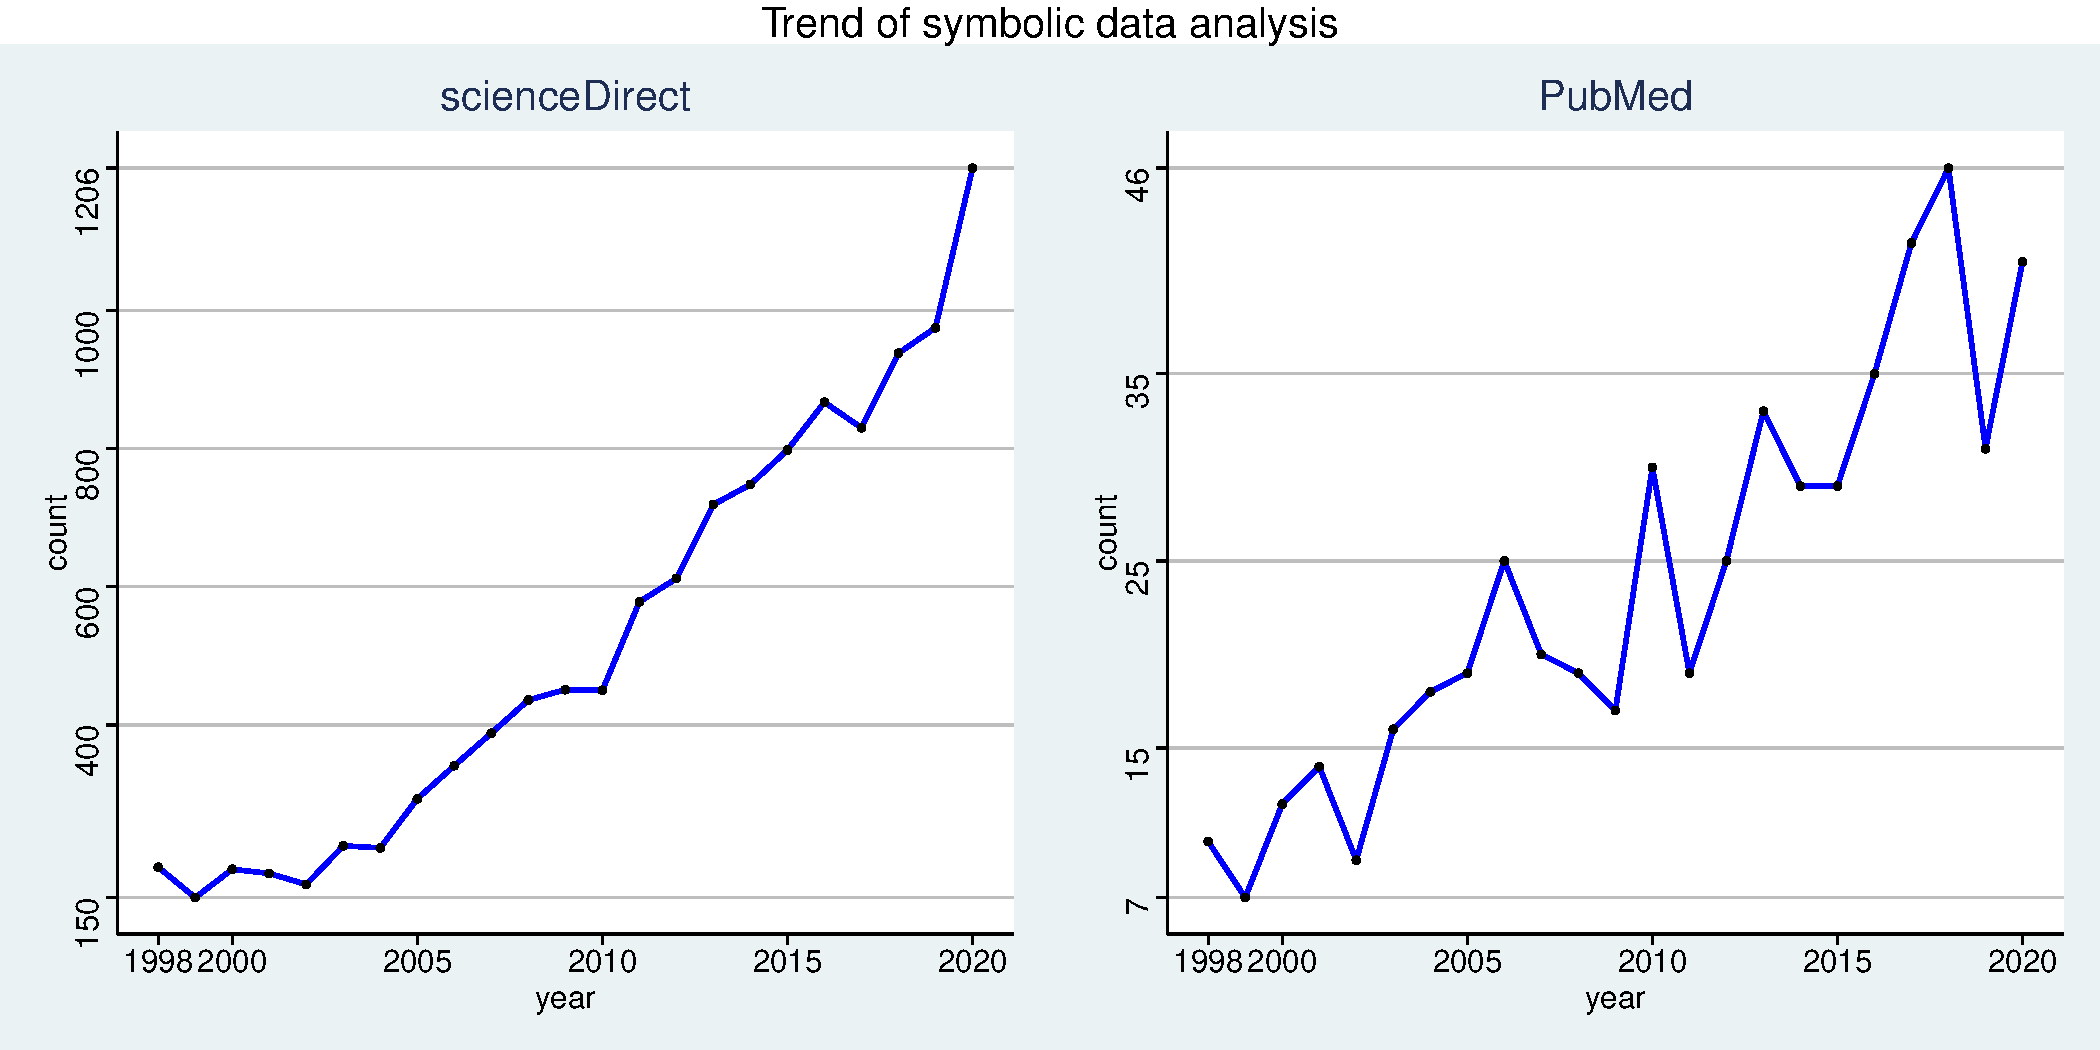
\includegraphics[width=1\textwidth]{pic/TrendFig}
\caption{\label{fig:trend}The number of "symbolic data analysis" or "interval-valued data" related articles in researches and applications according to PubMed and ScienceDirect online database over time from 1998 to 2020.}
\end{figure}



%%%%%%%%%%%%%%%%%%%%%%%%%%%
% Figure                  %
%%%%%%%%%%%%%%%%%%%%%%%%%%%
\begin{figure}[t!]
\centering	 		
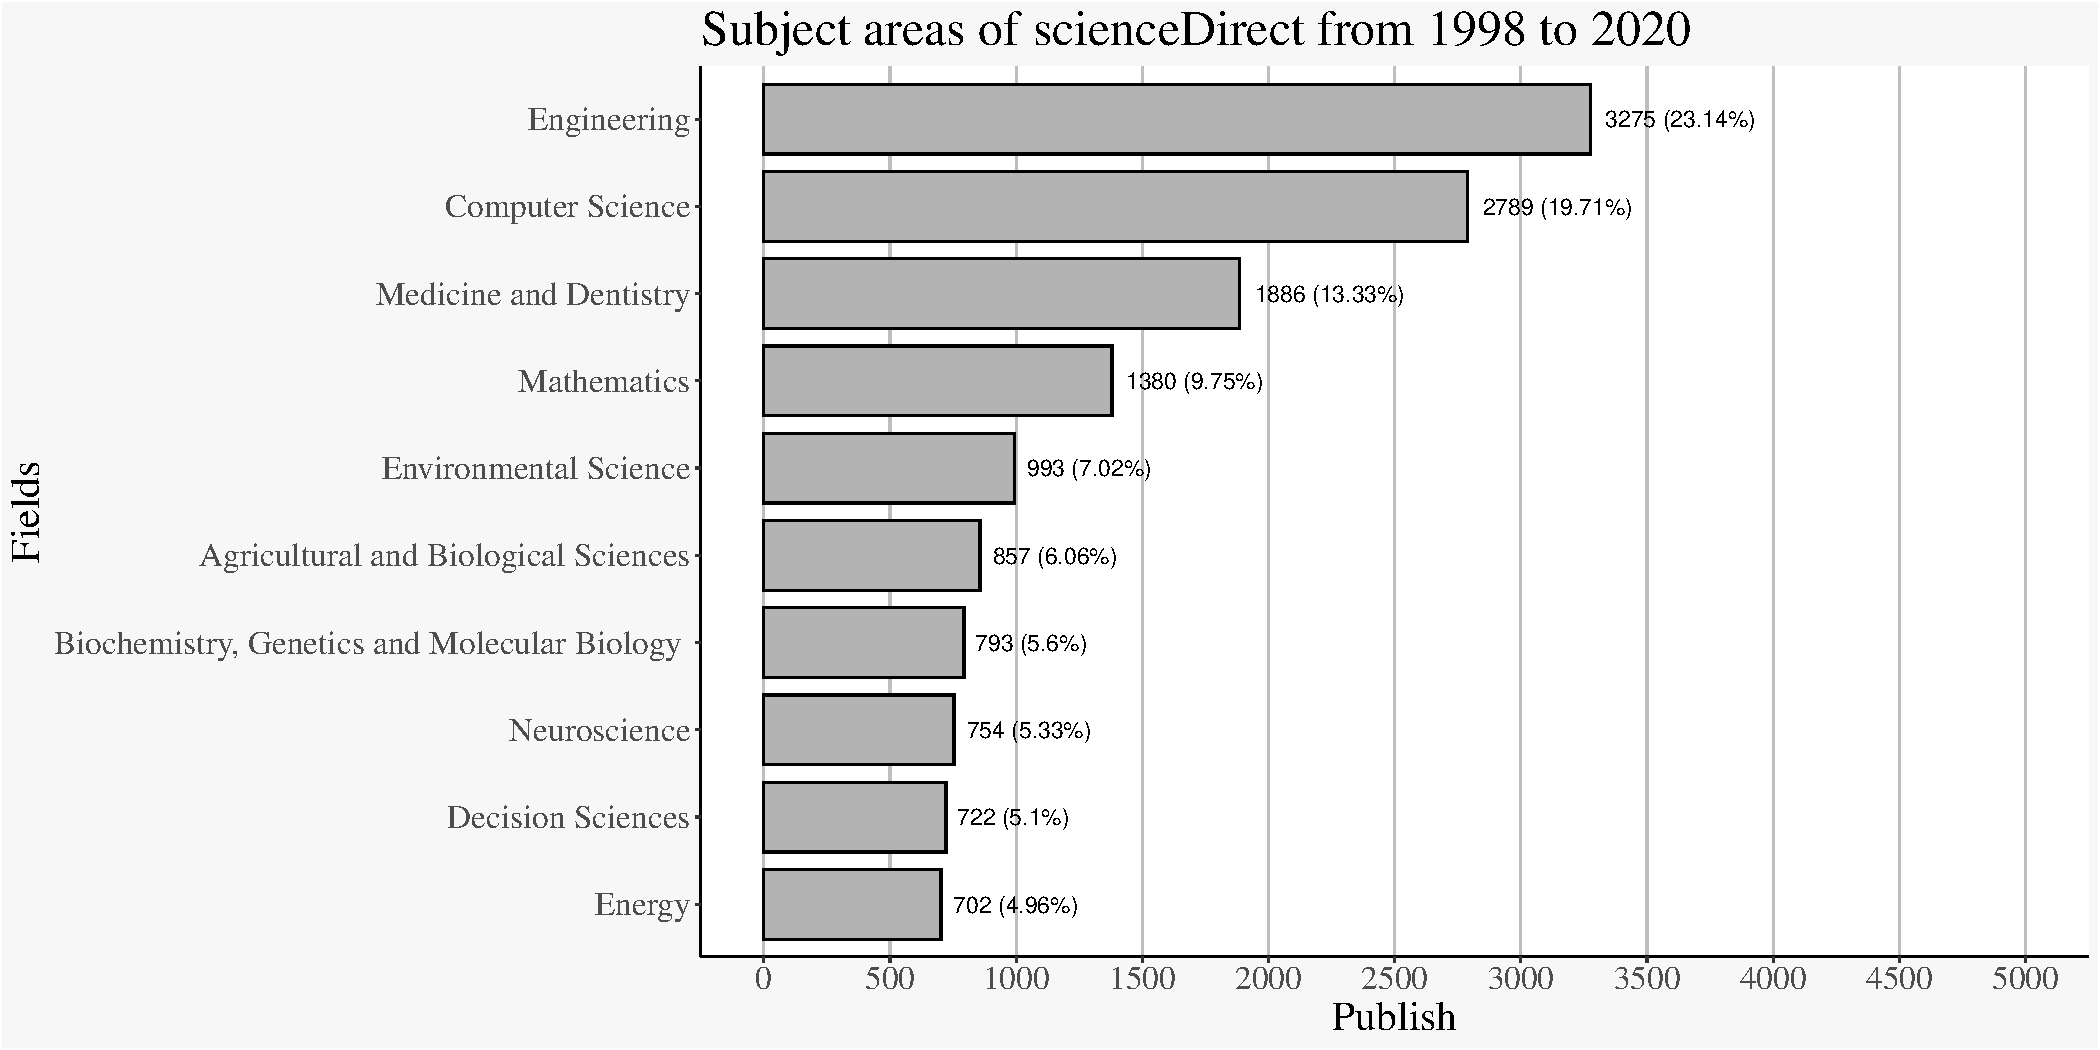
\includegraphics[width=1\textwidth]{pic/subjectFig} 
\caption{\label{fig:subjectAreas} Top 10 researches and applications domains for SDA or interval-valued data (ScienceDirect) from 1998 to 2020}  		   			 		 
\end{figure}



%%%%%%%%%%%%%%%%%%%%%%%%%%%
% Figure                  %
%%%%%%%%%%%%%%%%%%%%%%%%%%%
\begin{figure}[t!]
\centering	 			 	
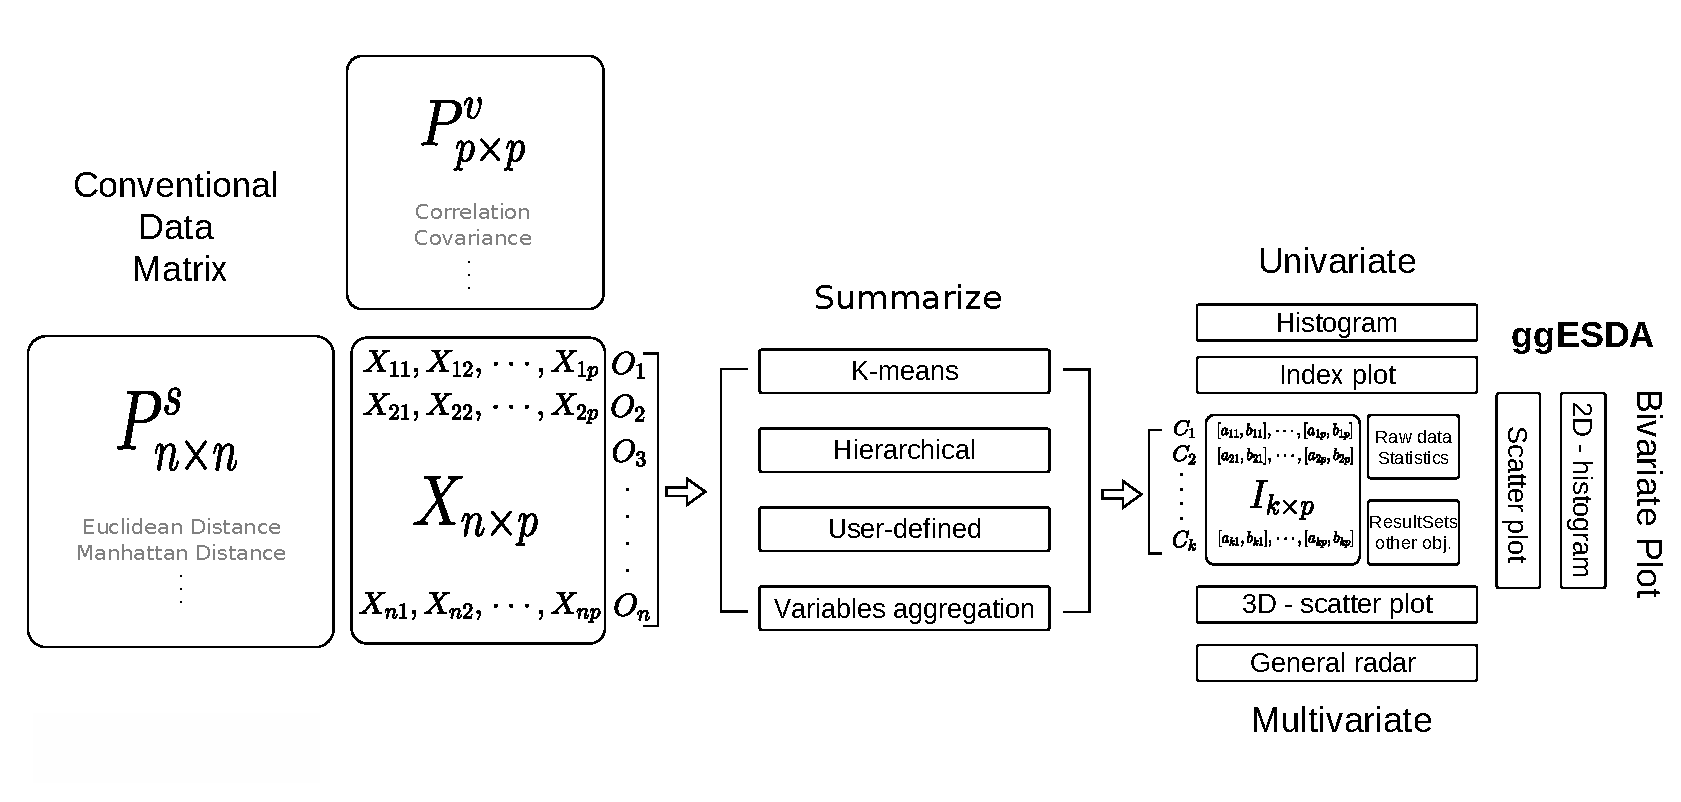
\includegraphics[width=1\textwidth]{pic/packageStructure2} 
\caption{\label{fig:pkgStr} Package Structure and Diagram for the Transformation Flow}  
\end{figure}



%%%%%%%%%%%%%%%%%%%%%%%%%%%
% Figure                  %
%%%%%%%%%%%%%%%%%%%%%%%%%%%
\begin{figure}[t!]
\centering
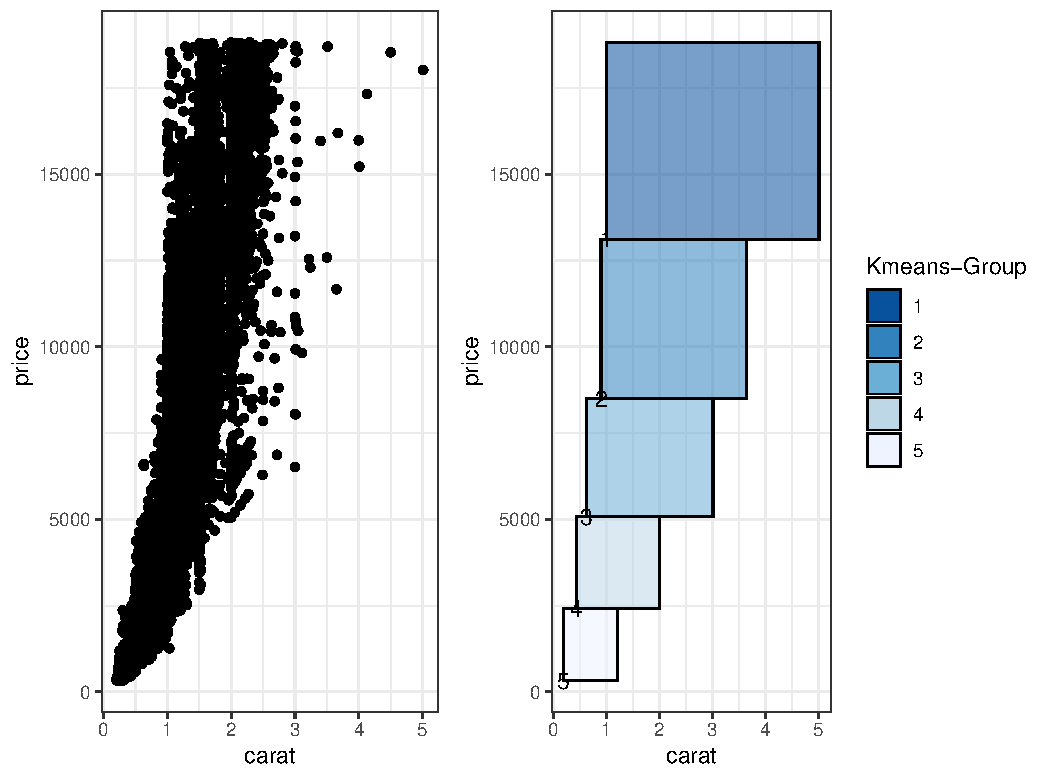
\includegraphics[width=1\textwidth]{pic/compare} 
\caption{\label{fig:compare} Compare classical data and symbolic data.}
\end{figure}



%%%%%%%%%%%%%%%%%%%%%%%%%%%
% Figure                  %
%%%%%%%%%%%%%%%%%%%%%%%%%%%
\begin{figure}[t!]
\centering
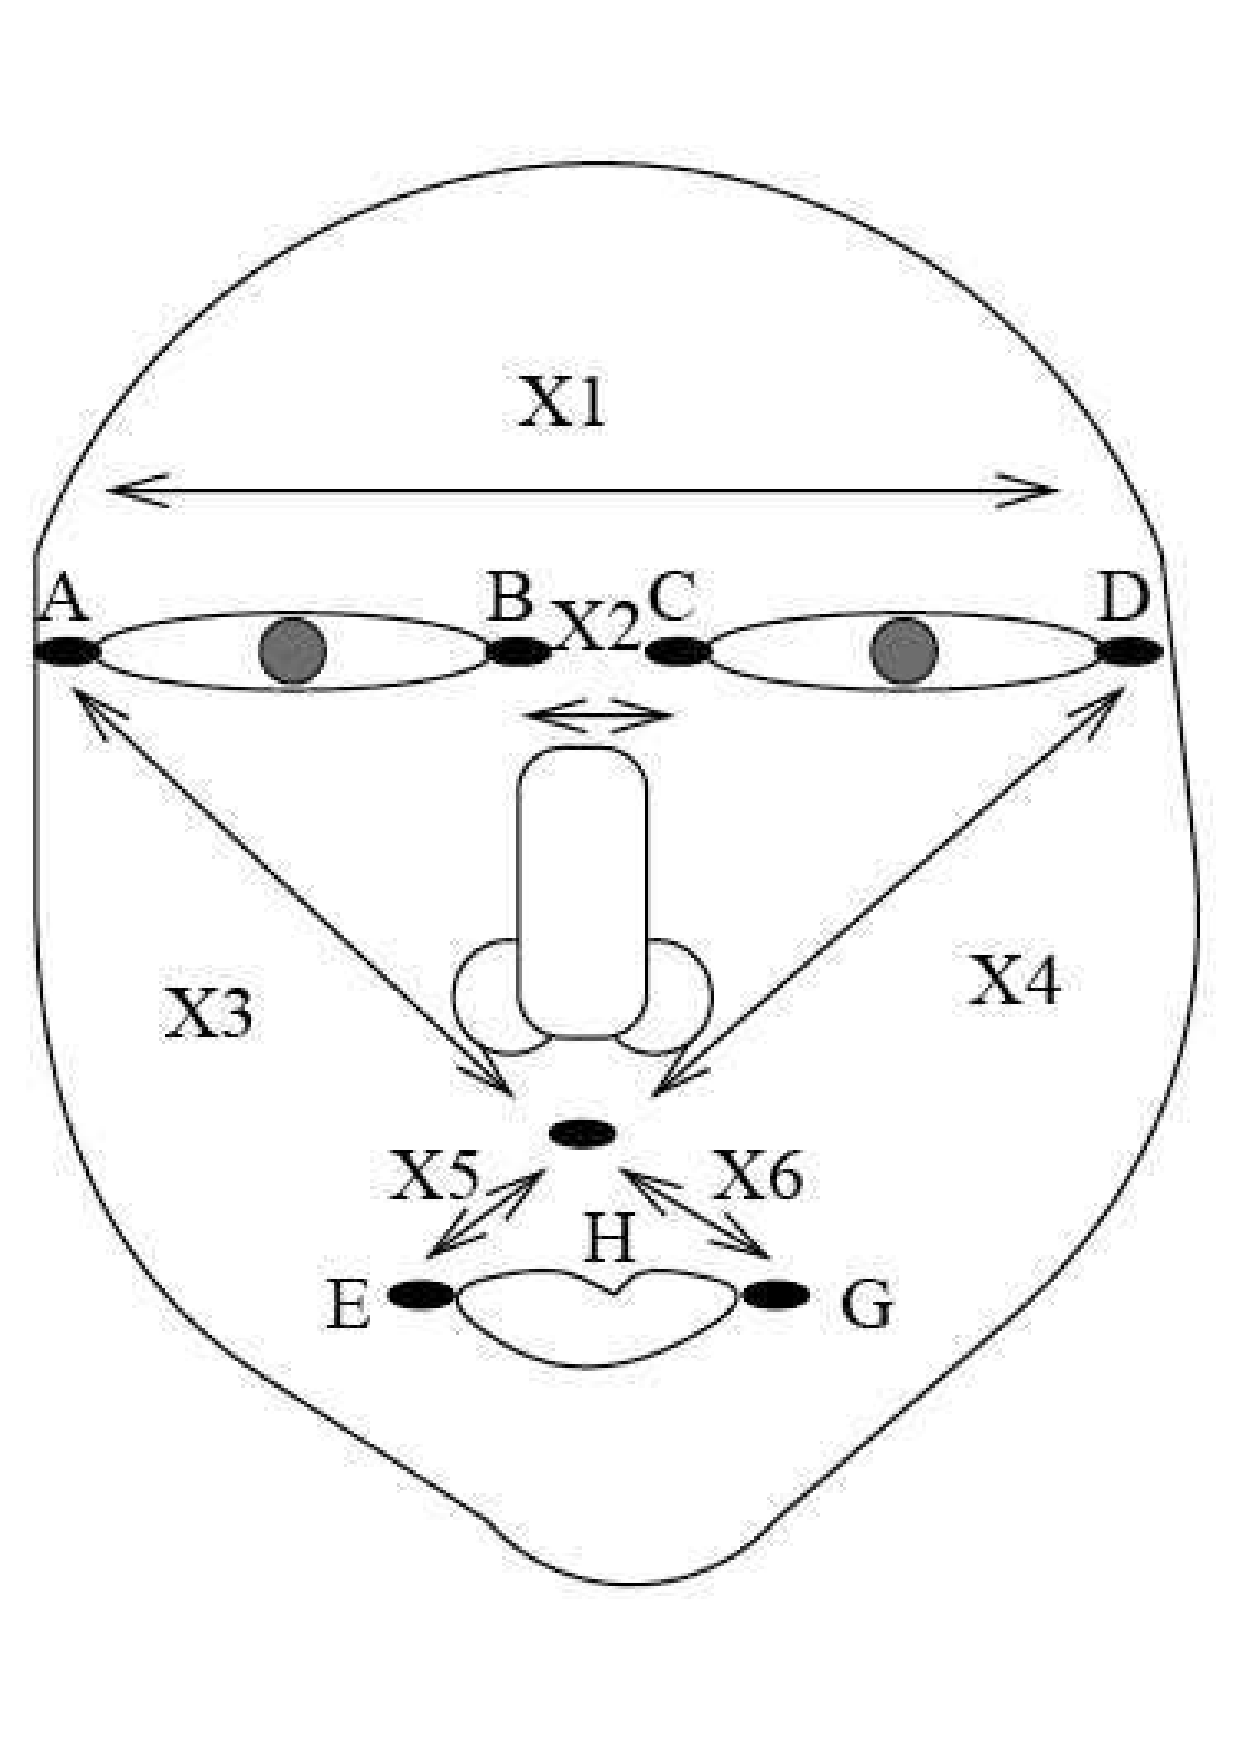
\includegraphics[width=0.5\textwidth]{pic/face}
\caption{\label{fig:face} The six face measurements for the face recognition dataset 
(Douzal-Chouakria, Billard and Diday, 2011).}
\end{figure}



%%%%%%%%%%%%%%%%%%%%%%%%%%%
% Figure                  %
%%%%%%%%%%%%%%%%%%%%%%%%%%%
\begin{figure}[t!]
\centering
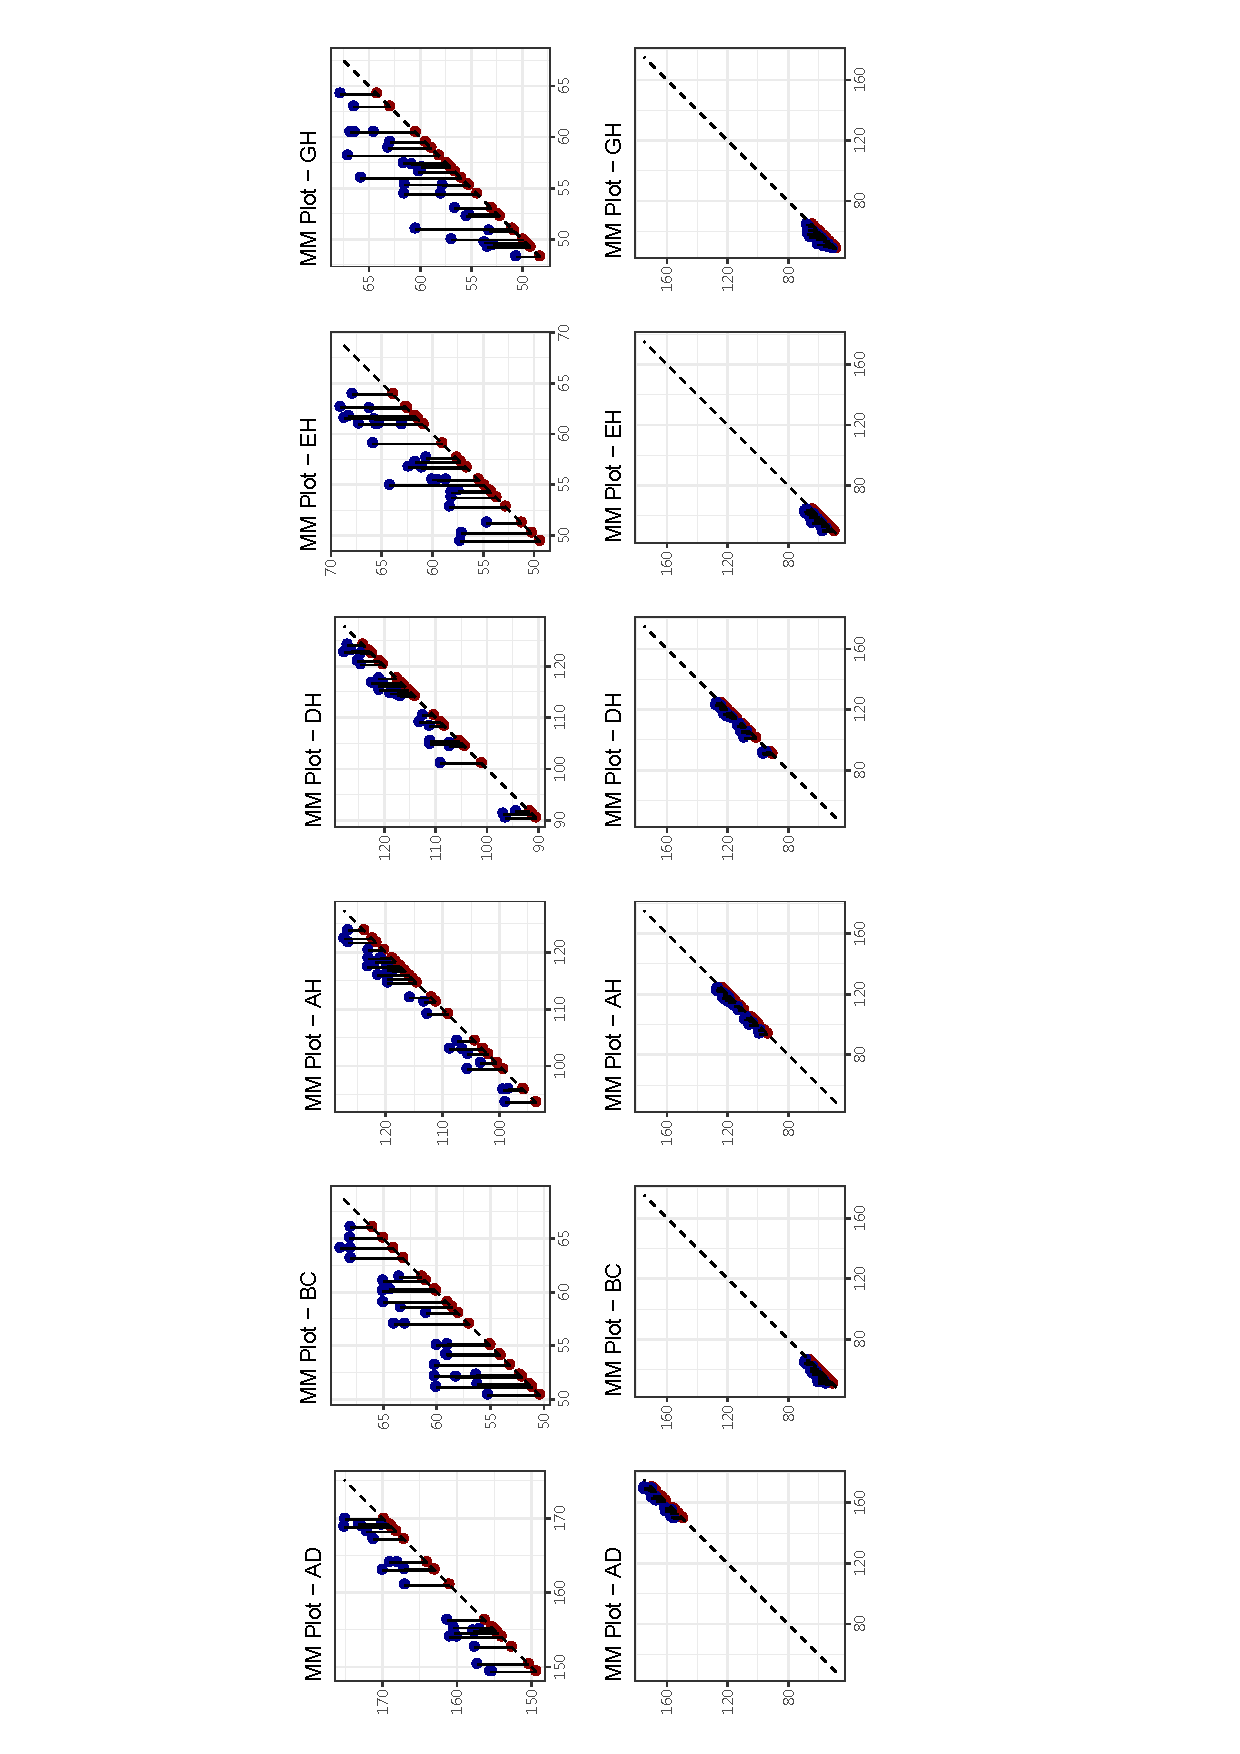
\includegraphics[width=1\textwidth]{pic/mmplot} 
\caption{\label{fig:minmax} The min-max plot. The figure in the top six conditions the axis in their own variables, whereas the bottom six conditions it in all variables.}
\end{figure}



%%%%%%%%%%%%%%%%%%%%%%%%%%%
% Figure                  %
%%%%%%%%%%%%%%%%%%%%%%%%%%%

\begin{figure}[t!]
\centering
\begin{tabular}{cc}
(a) & (b) \\
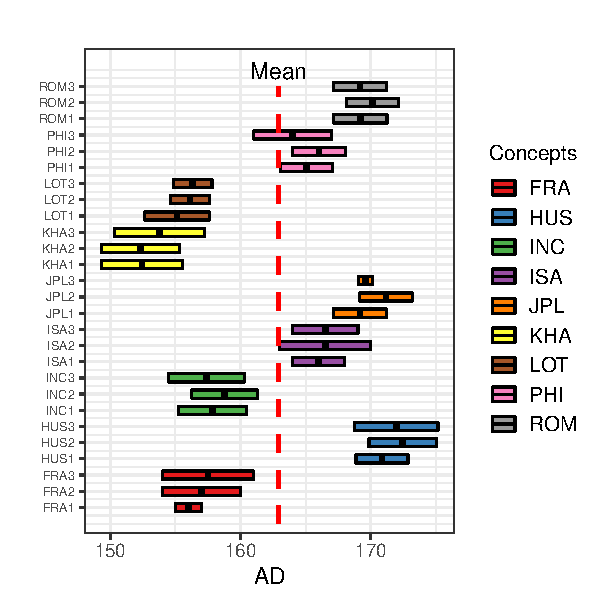
\includegraphics[width=0.5\textwidth]{pic/index_bar} &
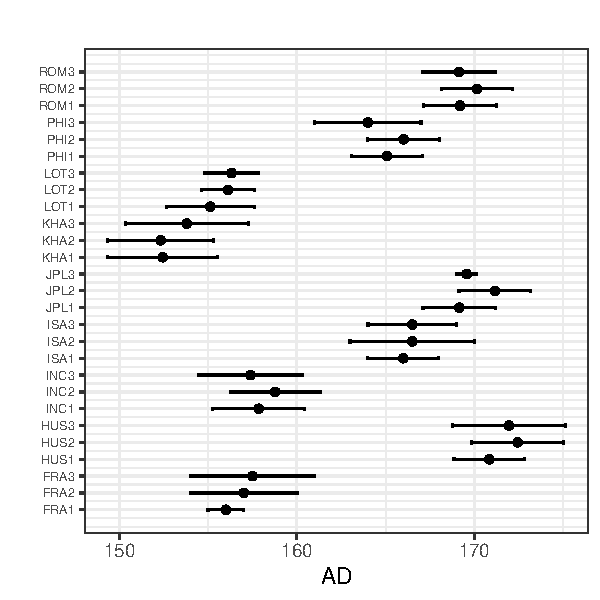
\includegraphics[width=0.5\textwidth]{pic/index} \\
(c) & (d) \\
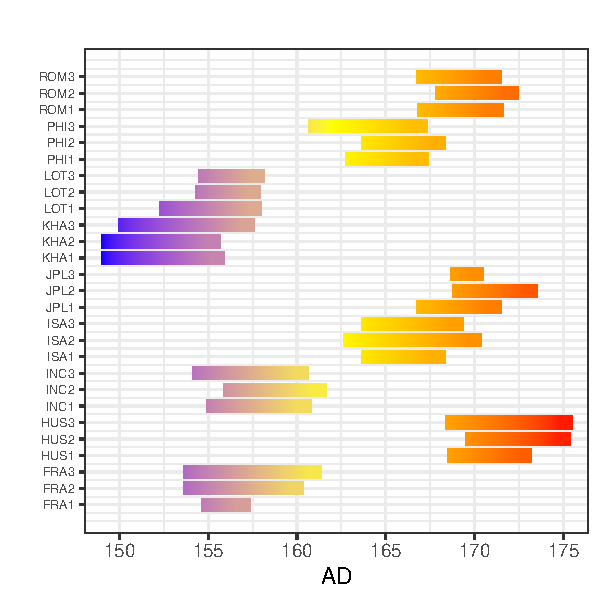
\includegraphics[width=0.5\textwidth]{pic/index_image1} &
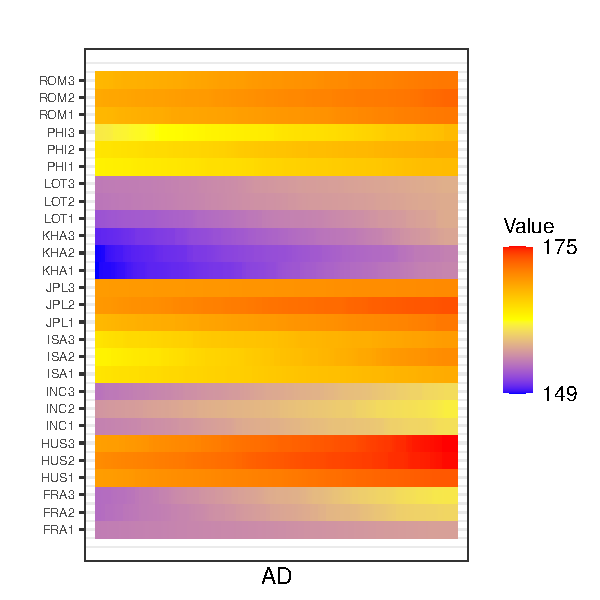
\includegraphics[width=0.5\textwidth]{pic/index_image2} 
\end{tabular}
\caption{\label{fig:index_full} Four kinds of index plot for the variable AD.
(a) Index plot, (b) Index plot with different group and common mean, (c) Index image,
and (d) Index image with extended color.}
\end{figure}

 

%%%%%%%%%%%%%%%%%%%%%%%%%%%
% Figure                  %
%%%%%%%%%%%%%%%%%%%%%%%%%%%
\begin{figure}[t!]
    \centering 
    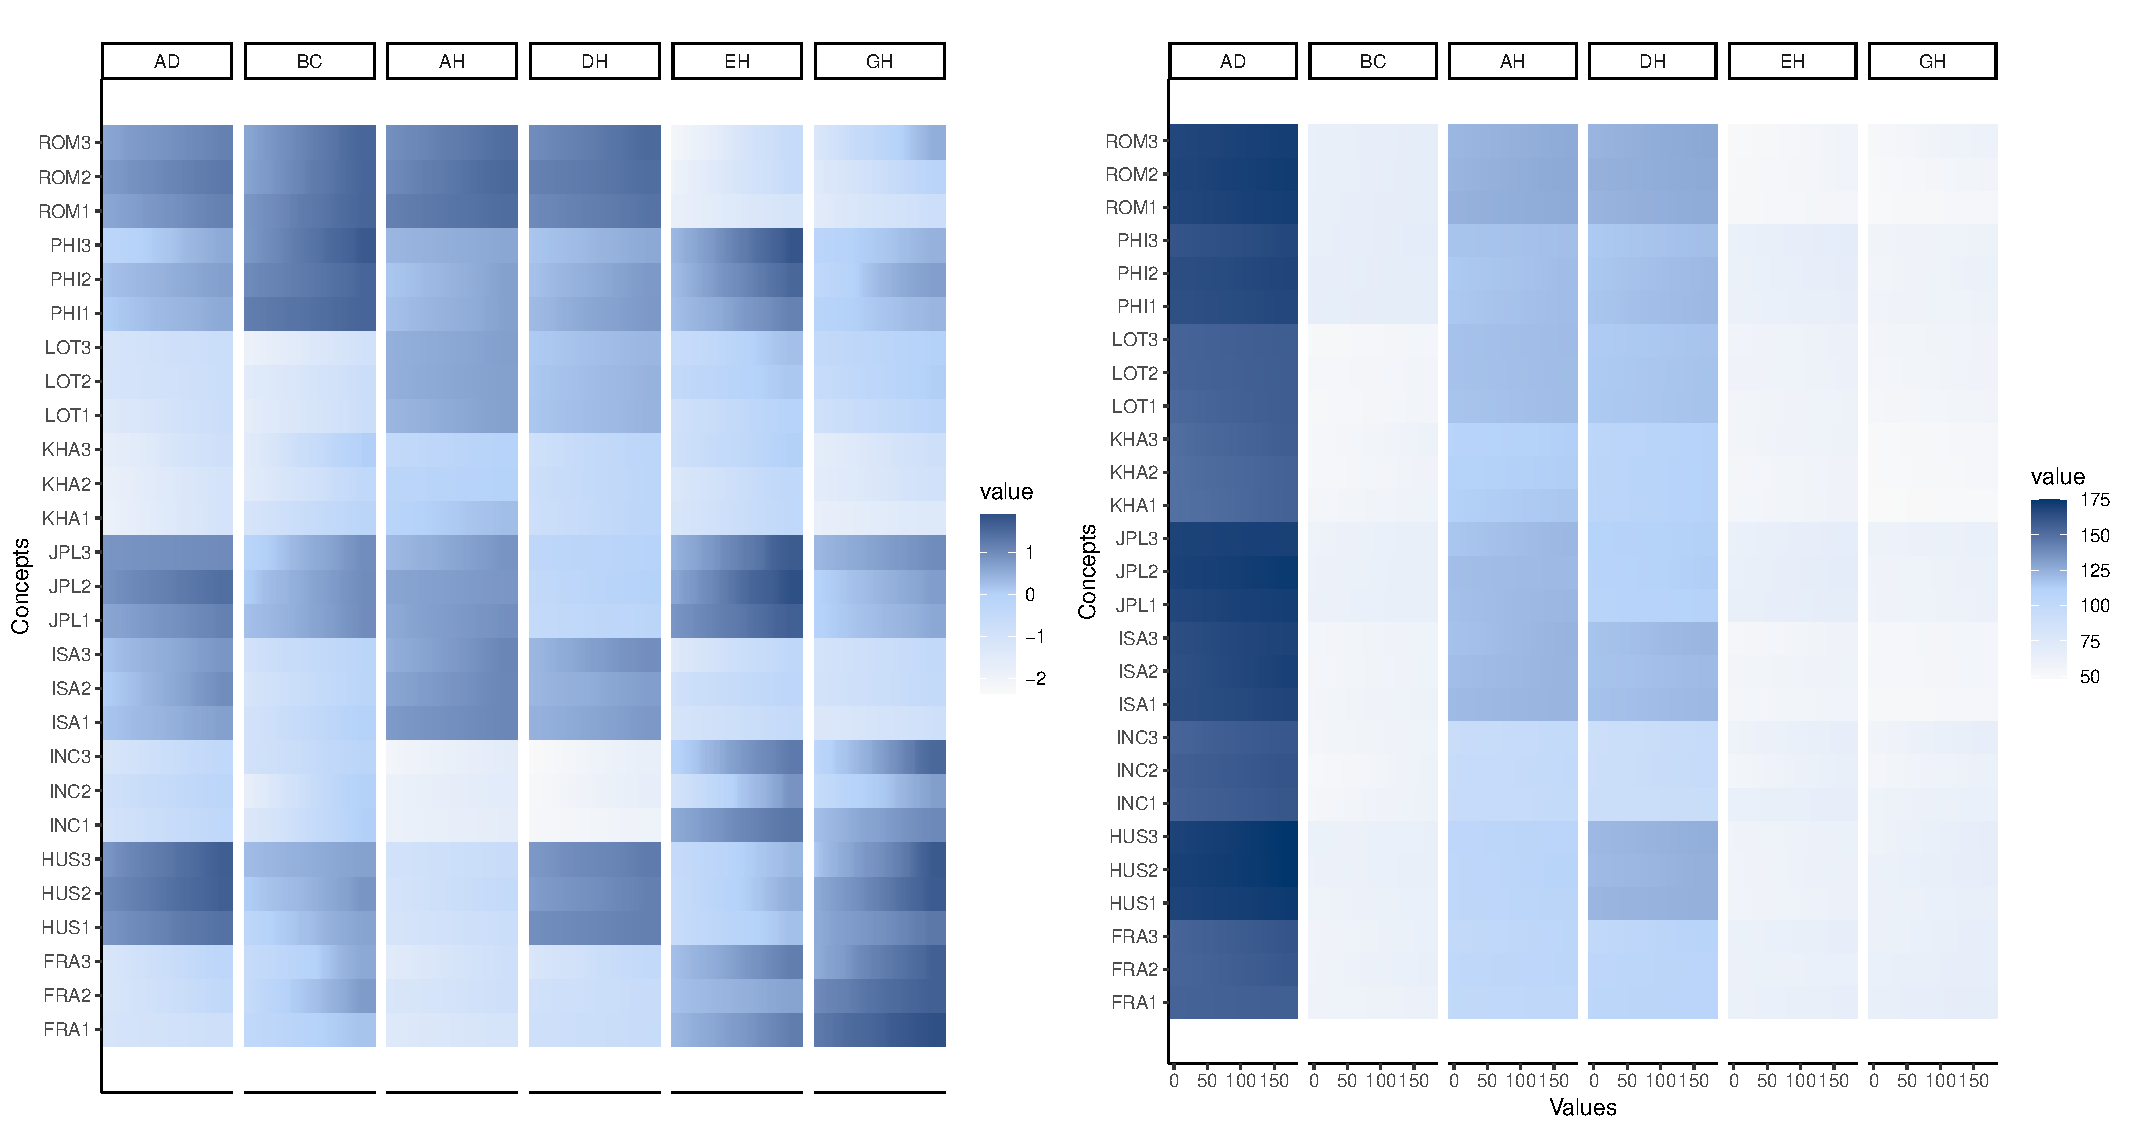
\includegraphics[width=1\textwidth]{pic/indexImage_2case}
    \caption{\label{fig:indexImage} Index image using a heatmap type.}
\end{figure}



%%%%%%%%%%%%%%%%%%%%%%%%%%%
% Figure                  %
%%%%%%%%%%%%%%%%%%%%%%%%%%%
\begin{figure}[t!]
\centering
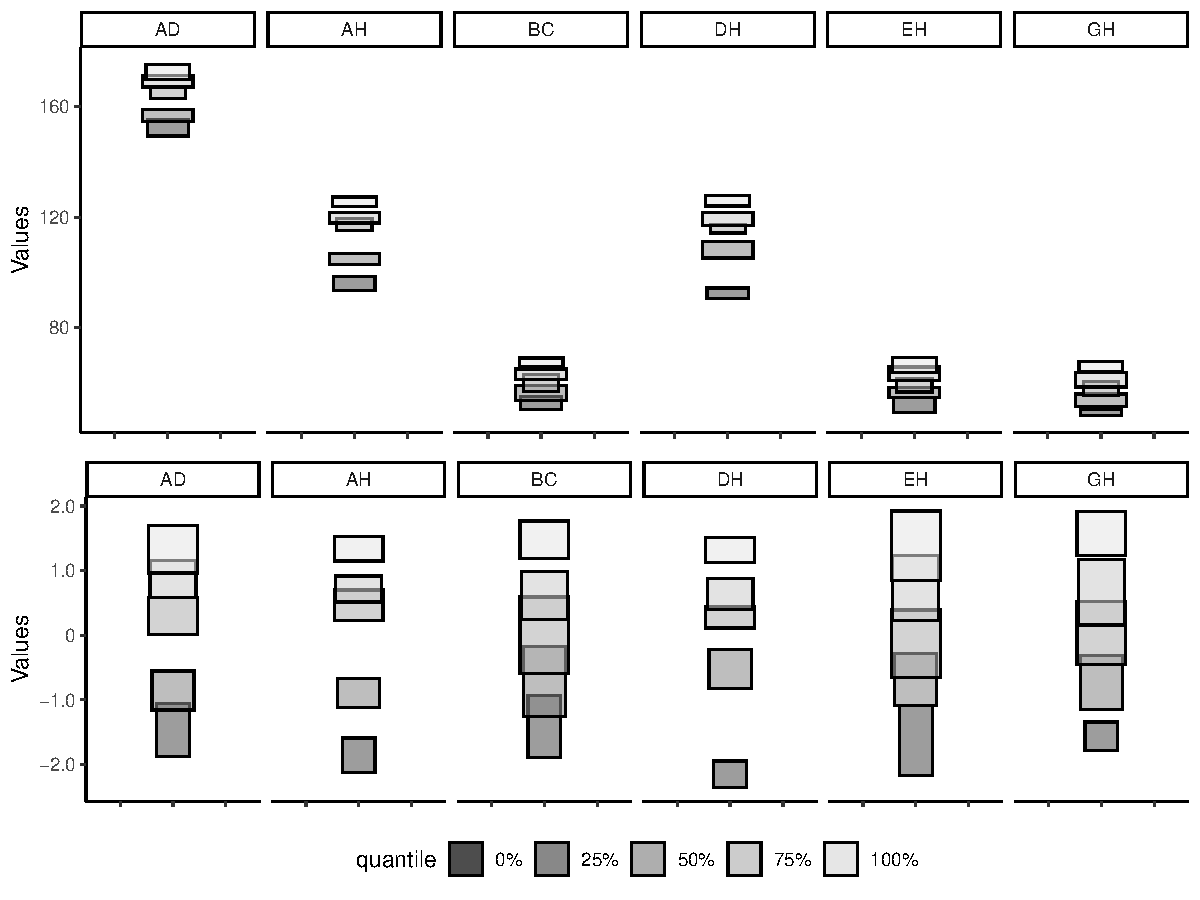
\includegraphics[width=1\textwidth]{pic/box_centerRange_before}
\caption{\label{fig:box} The side-by-side box plot. The figure in the top panel is the raw value of its variables, where the bottom panel is to standardize each variables.}
\end{figure}



%%%%%%%%%%%%%%%%%%%%%%%%%%%
% Figure                  %
%%%%%%%%%%%%%%%%%%%%%%%%%%%
\begin{figure}[t!]
\centering
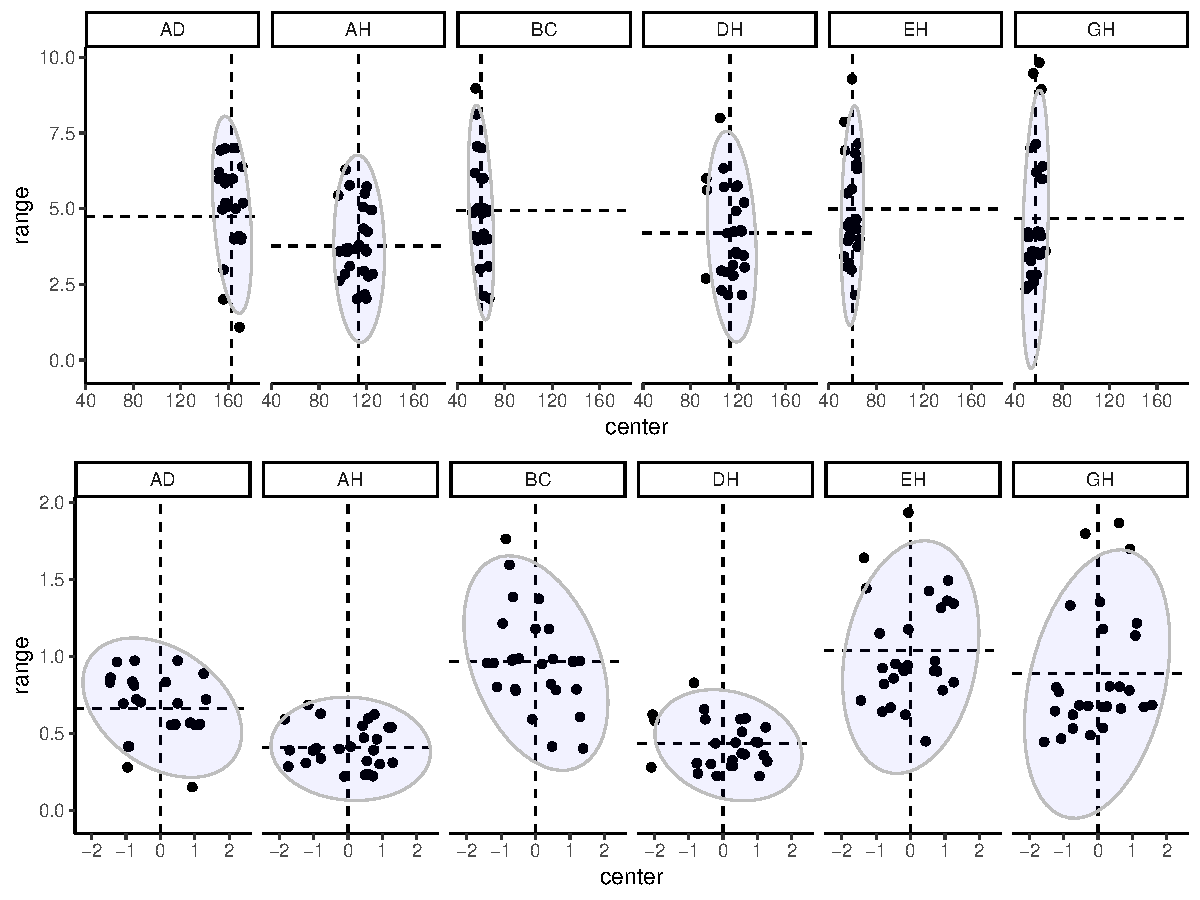
\includegraphics[width=1\textwidth]{pic/box_centerRange_after}
\caption{\label{fig:centerRange} The center-range plot.}
\end{figure}



%%%%%%%%%%%%%%%%%%%%%%%%%%%
% Figure                  %
%%%%%%%%%%%%%%%%%%%%%%%%%%%
\begin{figure}[t!]
\centering
\begin{tabular}{cc}
(a) & (b) \\
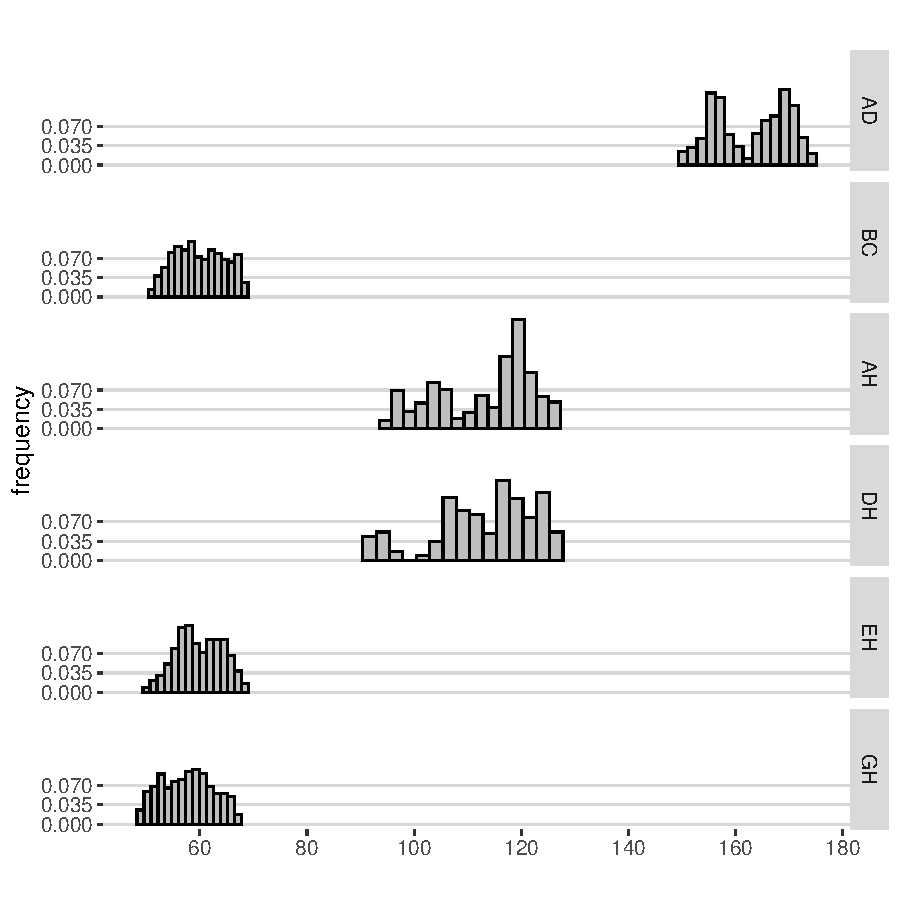
\includegraphics[width=0.5\textwidth]{pic/hist_equal} &
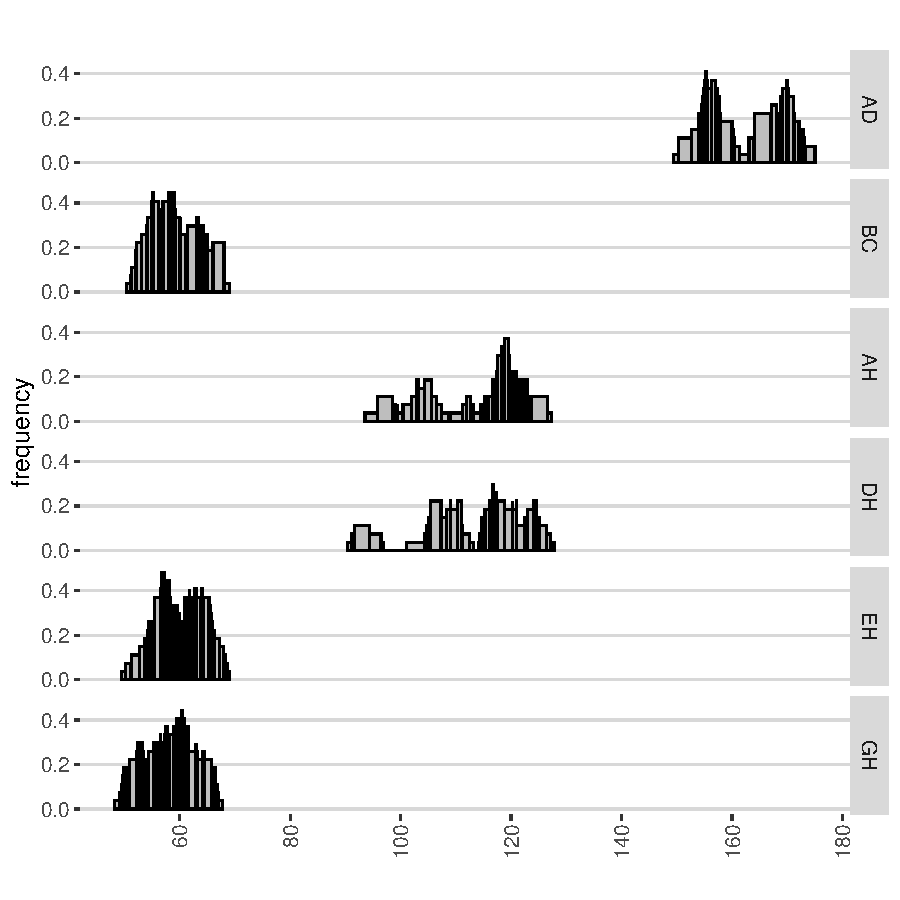
\includegraphics[width=0.5\textwidth]{pic/hist_unequal}
\end{tabular}
\caption{\label{fig:hist} (a) Equidistant-bin histogram. (b) Non-equidistant-bin histogram.}
\end{figure}



%%%%%%%%%%%%%%%%%%%%%%%%%%%
% Figure                  %
%%%%%%%%%%%%%%%%%%%%%%%%%%%
\begin{figure}[t!]
\centering
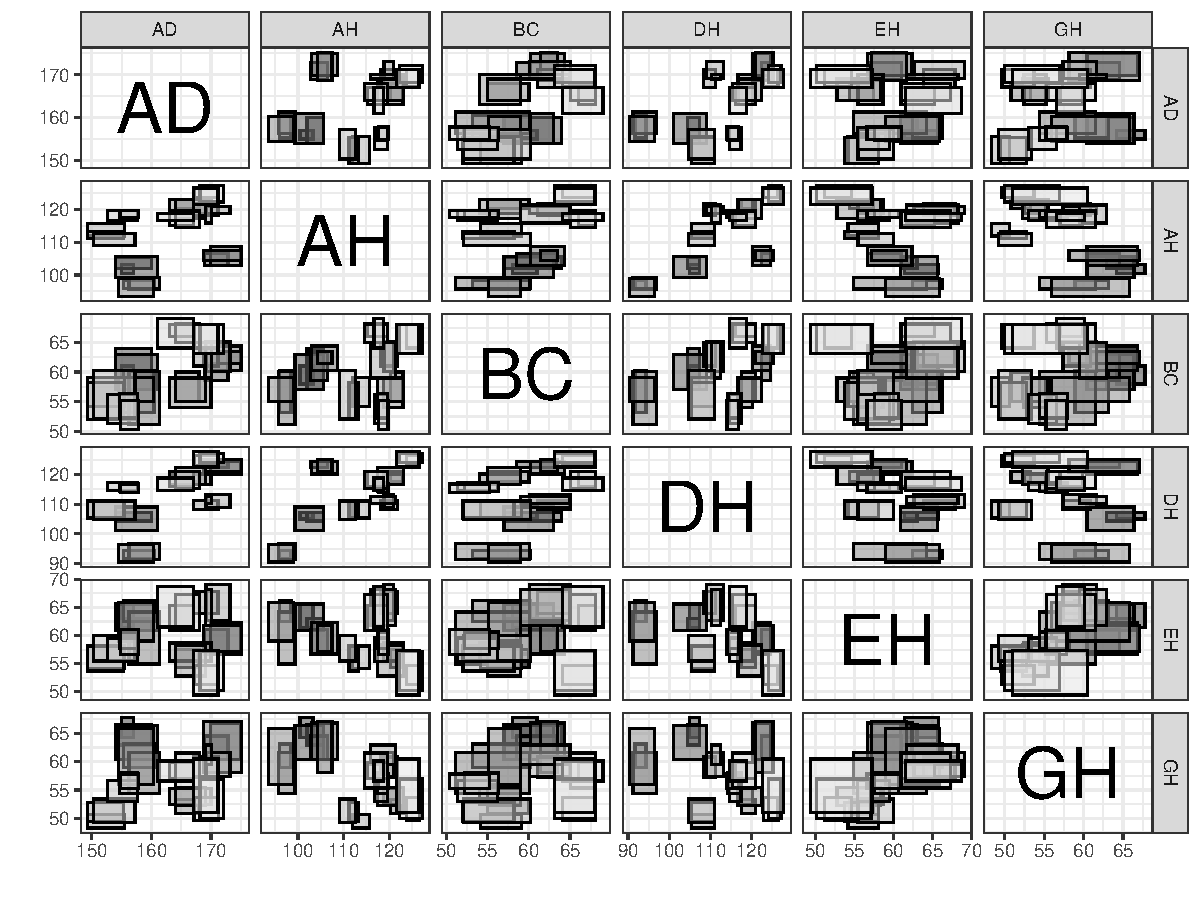
\includegraphics[width=1\textwidth]{pic/scaMatrix}
\caption{\label{fig:scaMatrix} Scatter matrix}
\end{figure}



%%%%%%%%%%%%%%%%%%%%%%%%%%%
% Figure                  %
%%%%%%%%%%%%%%%%%%%%%%%%%%%
\begin{figure}[t!]
\begin{center}
\begin{tabular}{cc}
(a) & (b) \\
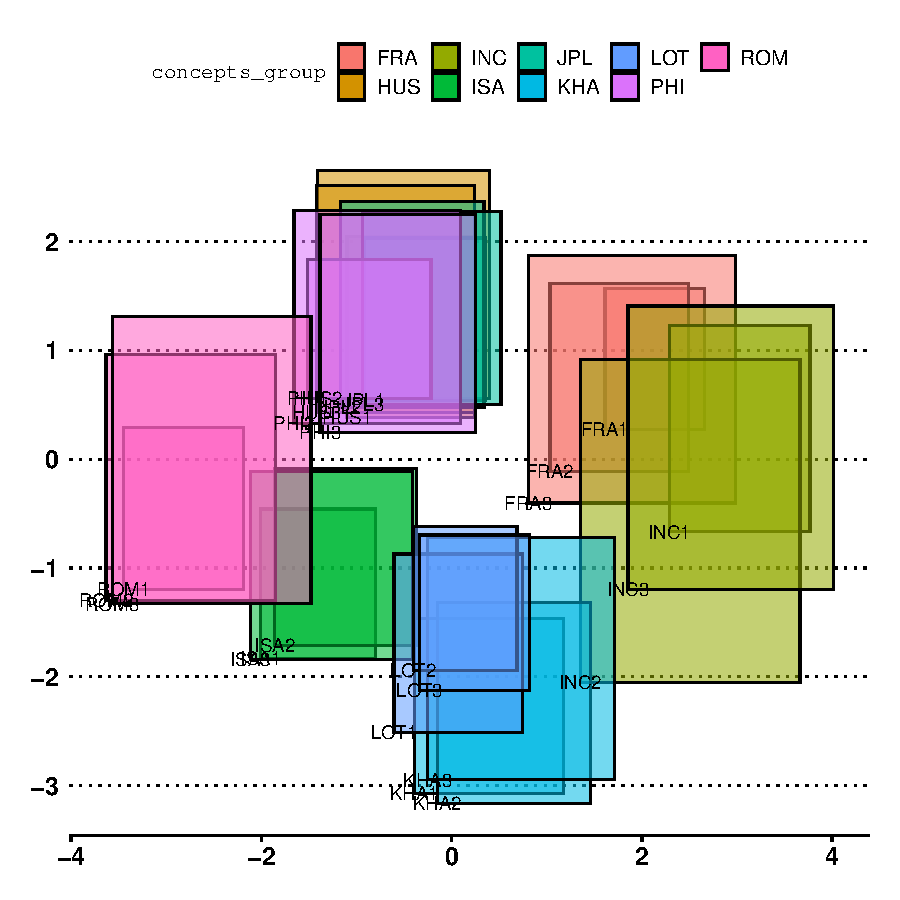
\includegraphics[width=0.5\textwidth]{pic/PCA_MCAR} &
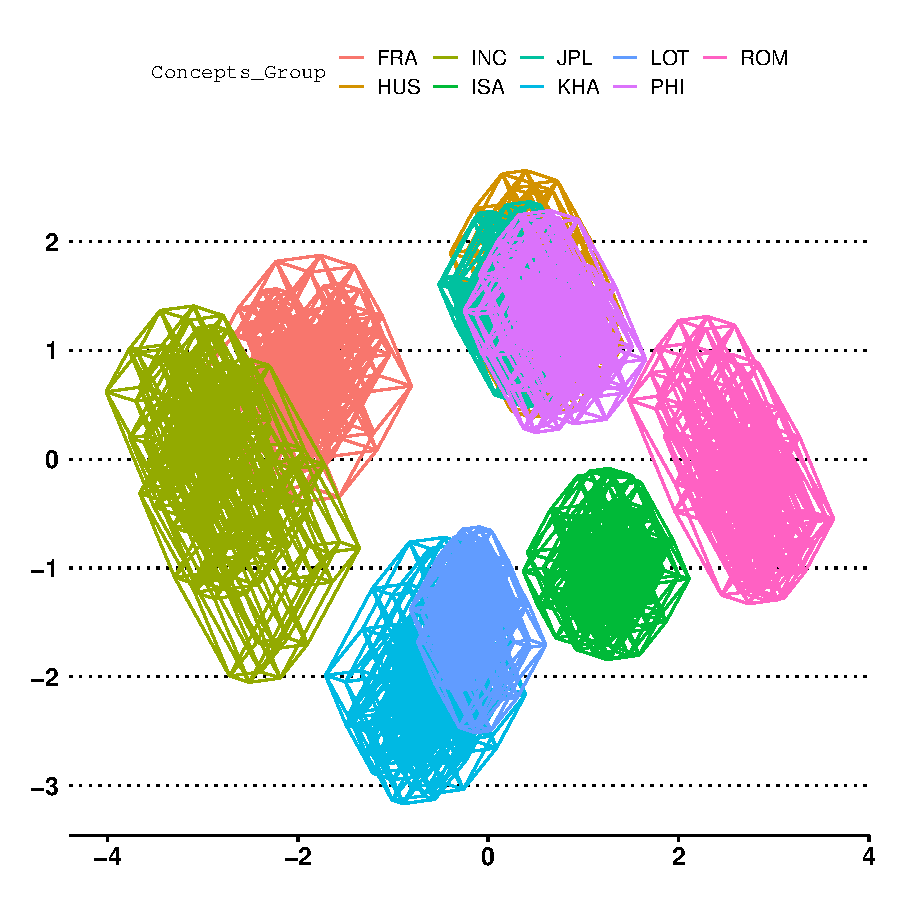
\includegraphics[width=0.5\textwidth]{pic/PCA_Polytope}
\end{tabular}
\caption{\label{fig:PCA} Two kinks of PCA for interval-valued data, where the XY-axis are represent the first principal component and the second principal component, respectively.
(Vertice-PCA (MCAR). (b) Vertice-PCA (Polytope)}
\end{center}
\end{figure}



%%%%%%%%%%%%%%%%%%%%%%%%%%%
% Figure                  %
%%%%%%%%%%%%%%%%%%%%%%%%%%%
\begin{figure}[t!]
\centering
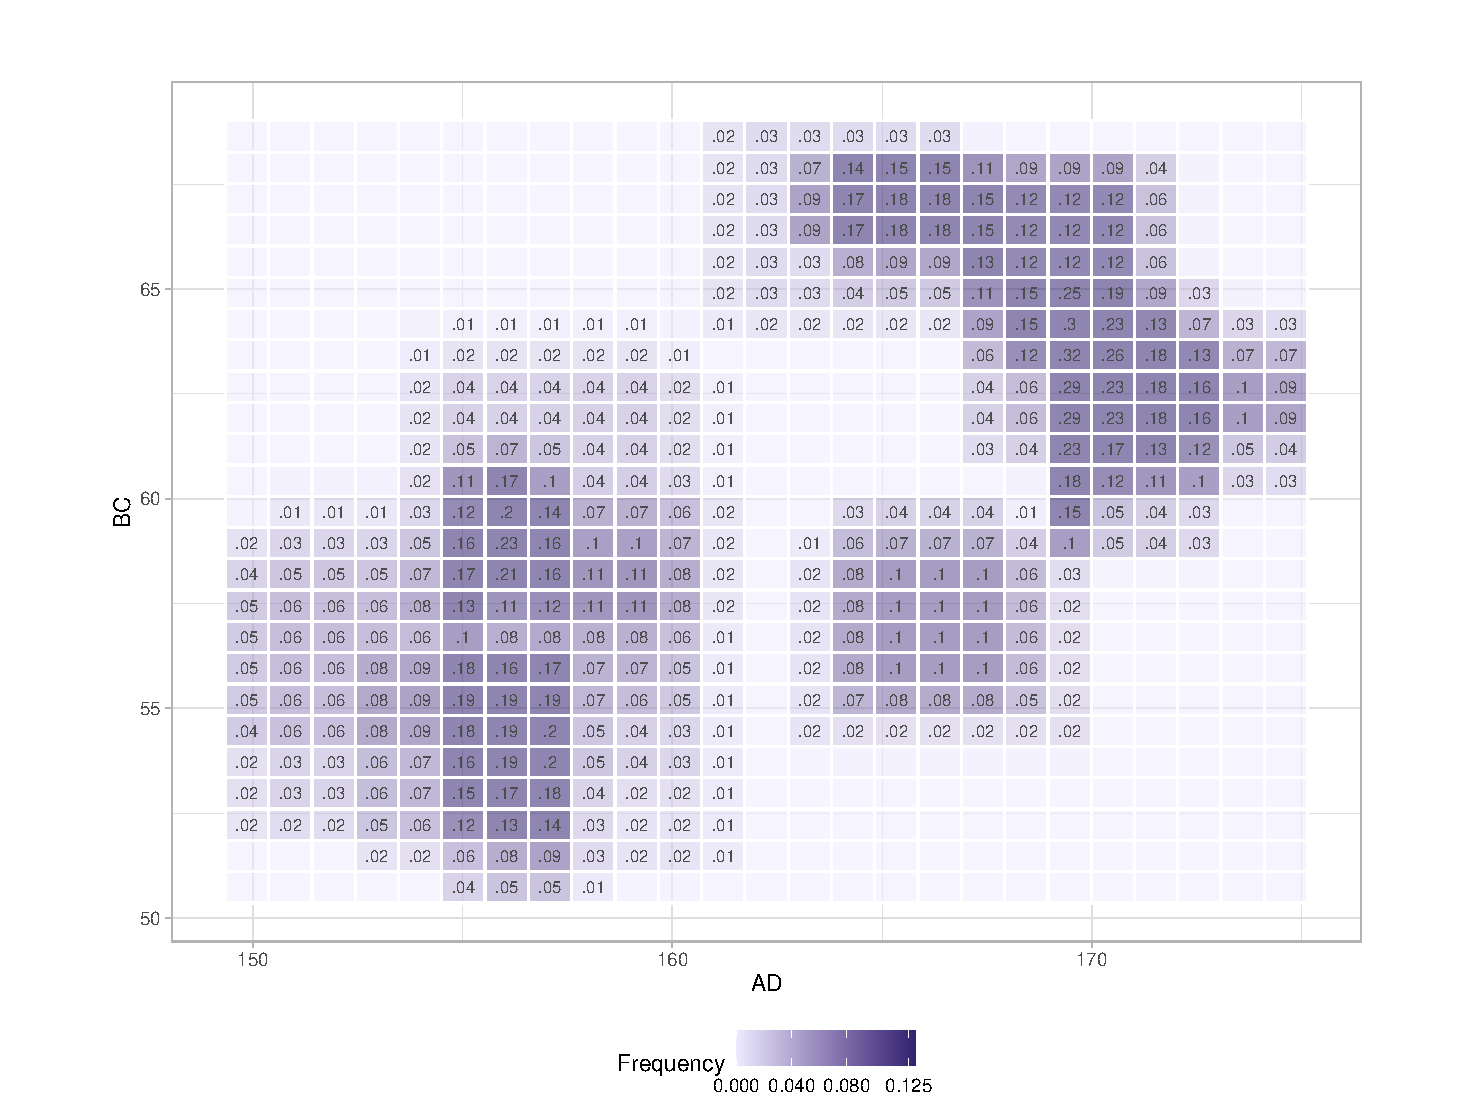
\includegraphics[width=1\textwidth]{pic/2Dhist}
\caption{\label{fig:2Dhist} 2D histogram.}
\end{figure}



%%%%%%%%%%%%%%%%%%%%%%%%%%%
% Figure                  %
%%%%%%%%%%%%%%%%%%%%%%%%%%%
\begin{figure}[t!]
\centering
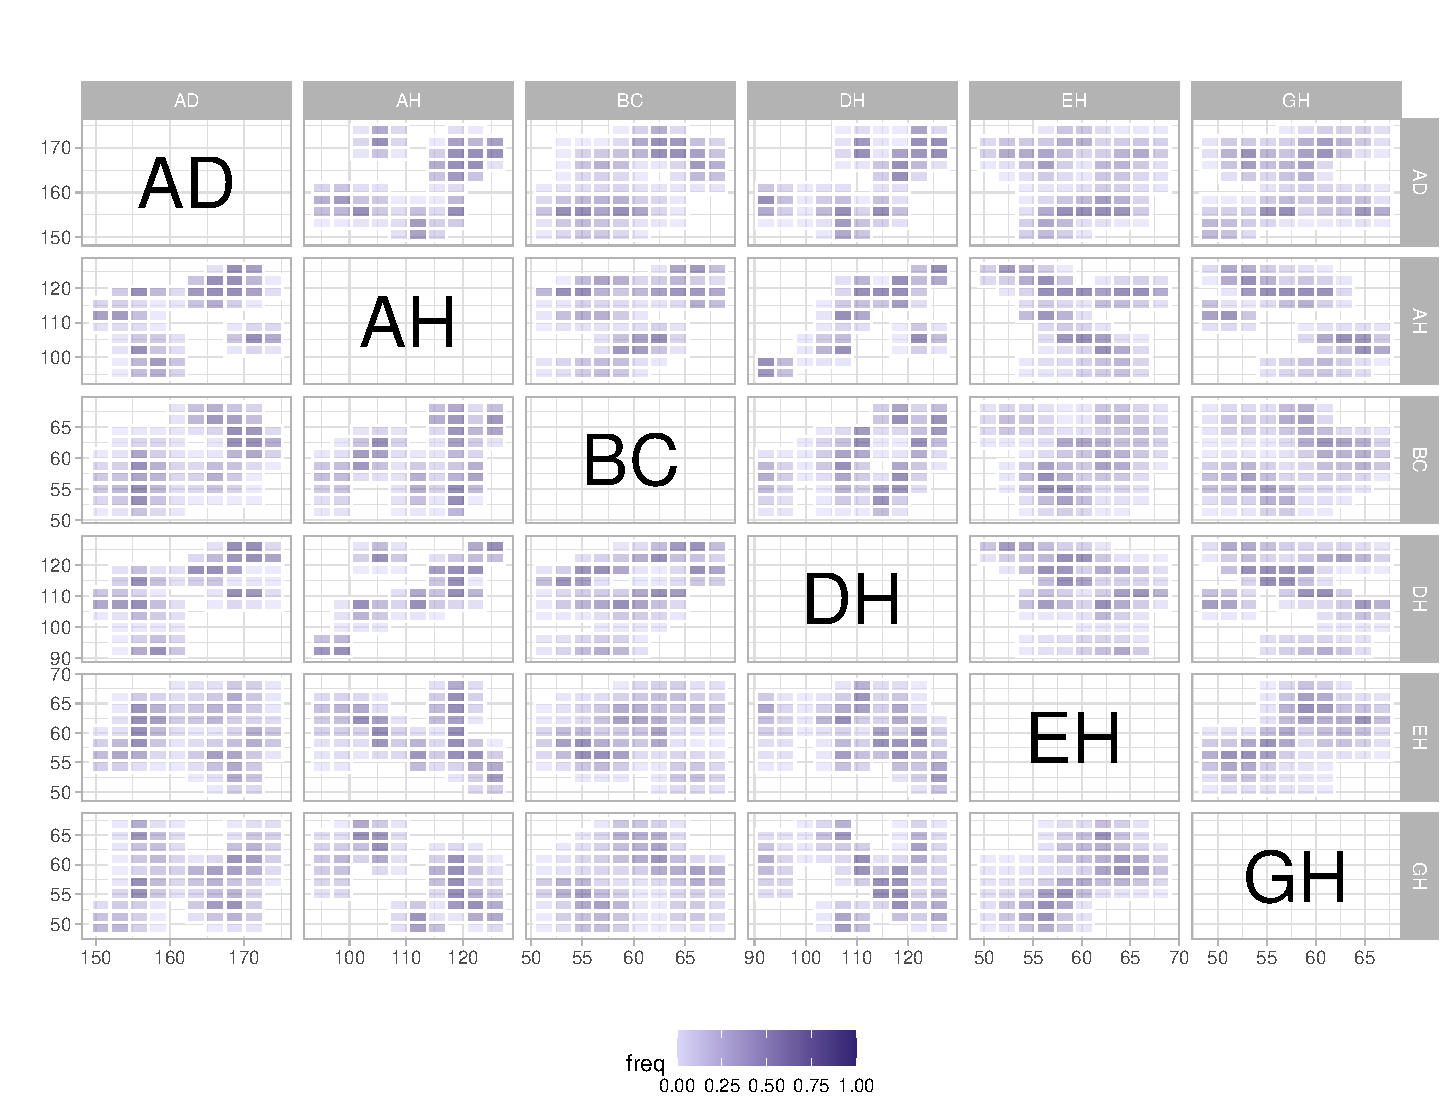
\includegraphics[width=1\textwidth]{pic/2DhistMatrix}
\caption{\label{fig:2DhistMatrix} 2D histogram matrix.}
\end{figure}



%%%%%%%%%%%%%%%%%%%%%%%%%%%
% Figure                  %
%%%%%%%%%%%%%%%%%%%%%%%%%%%
\begin{figure}[t!]
\centering
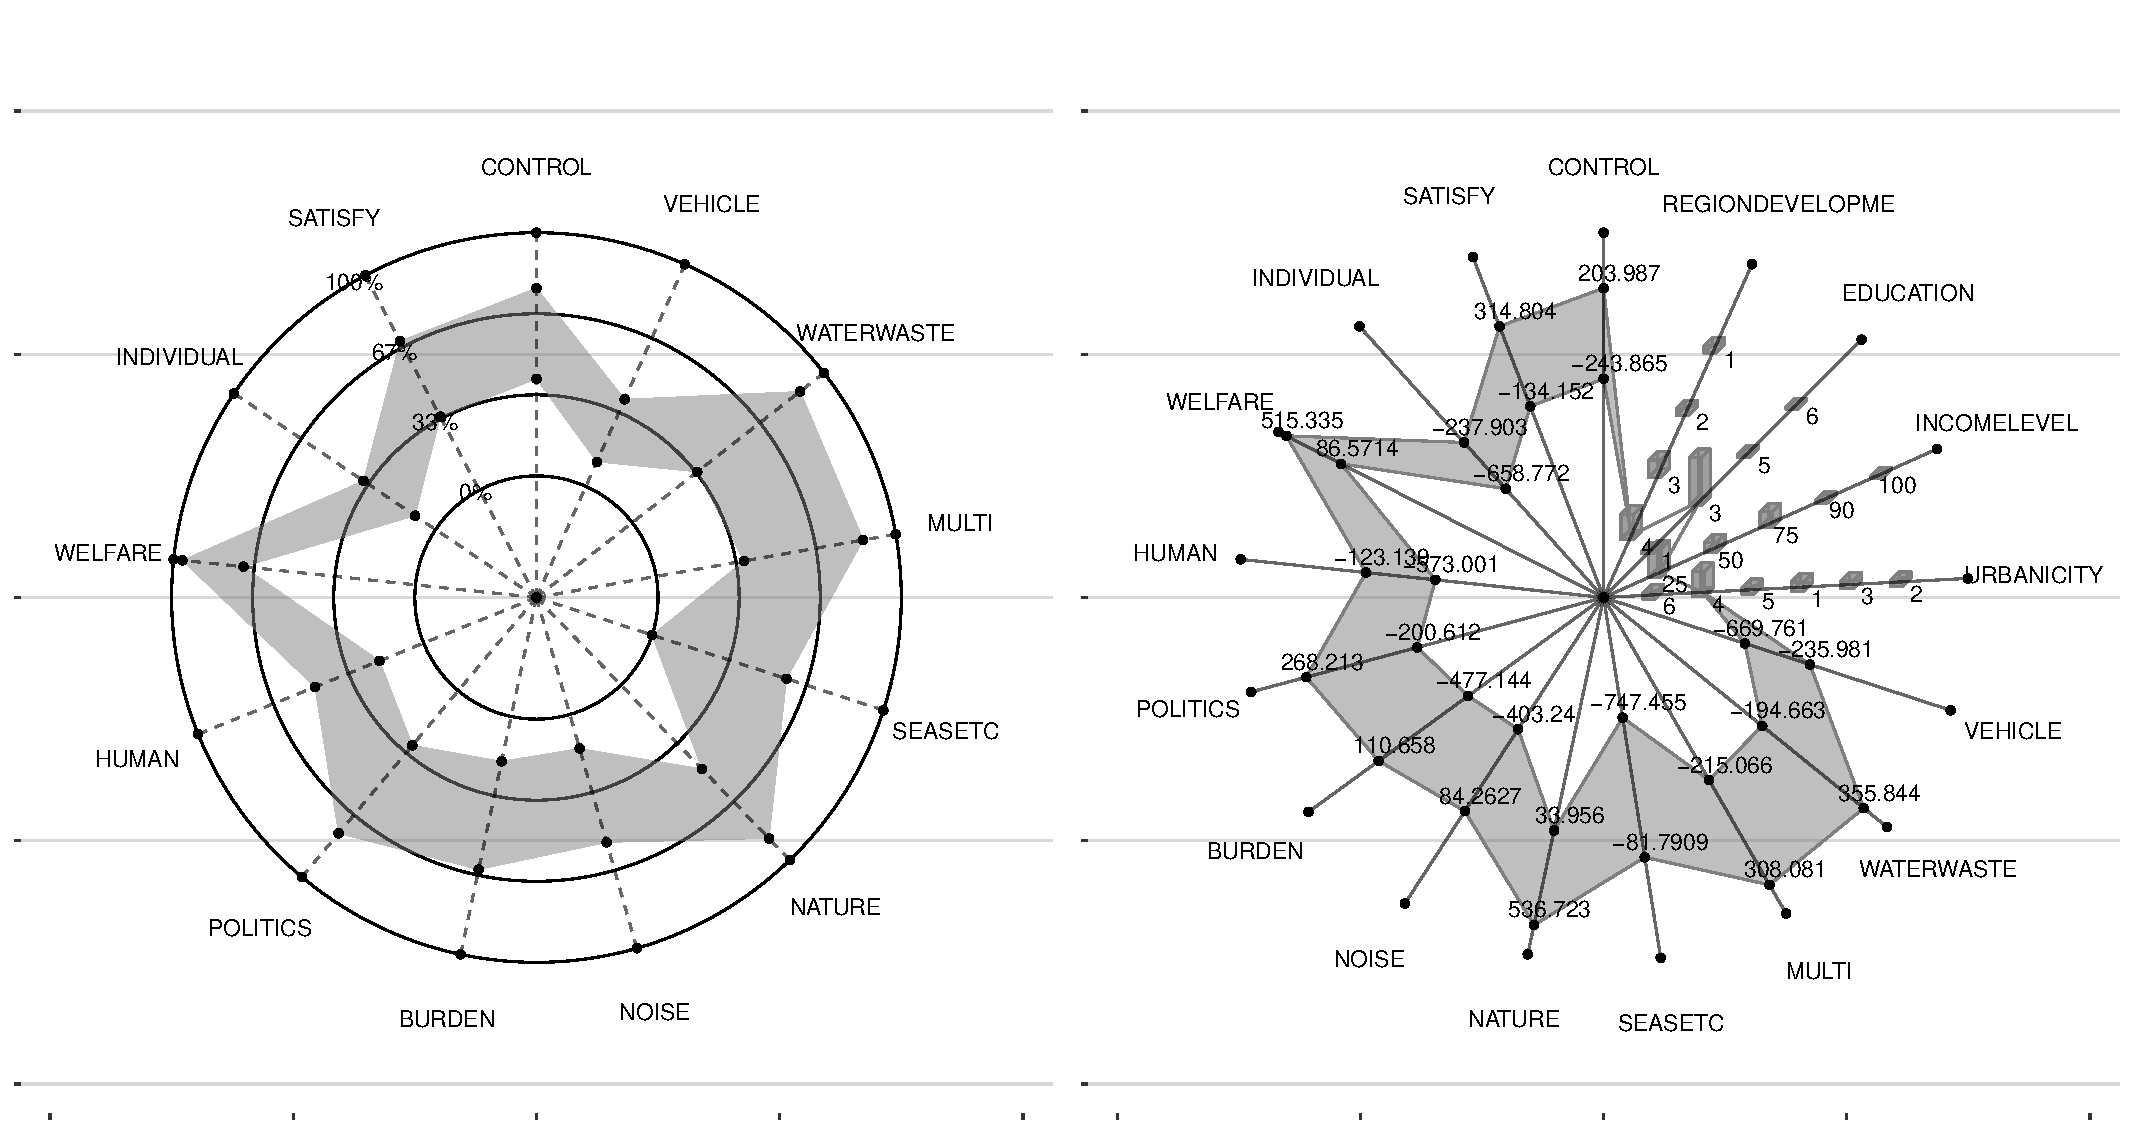
\includegraphics[width=1\textwidth]{pic/radar_typical} 
\caption{\label{fig:radar_typical} The variety of typical radar plot which is able to contain interval-valued and modal multi-valued variables.}
\end{figure}



%%%%%%%%%%%%%%%%%%%%%%%%%%%
% Figure                  %
%%%%%%%%%%%%%%%%%%%%%%%%%%%
\begin{figure}[t!]
\centering
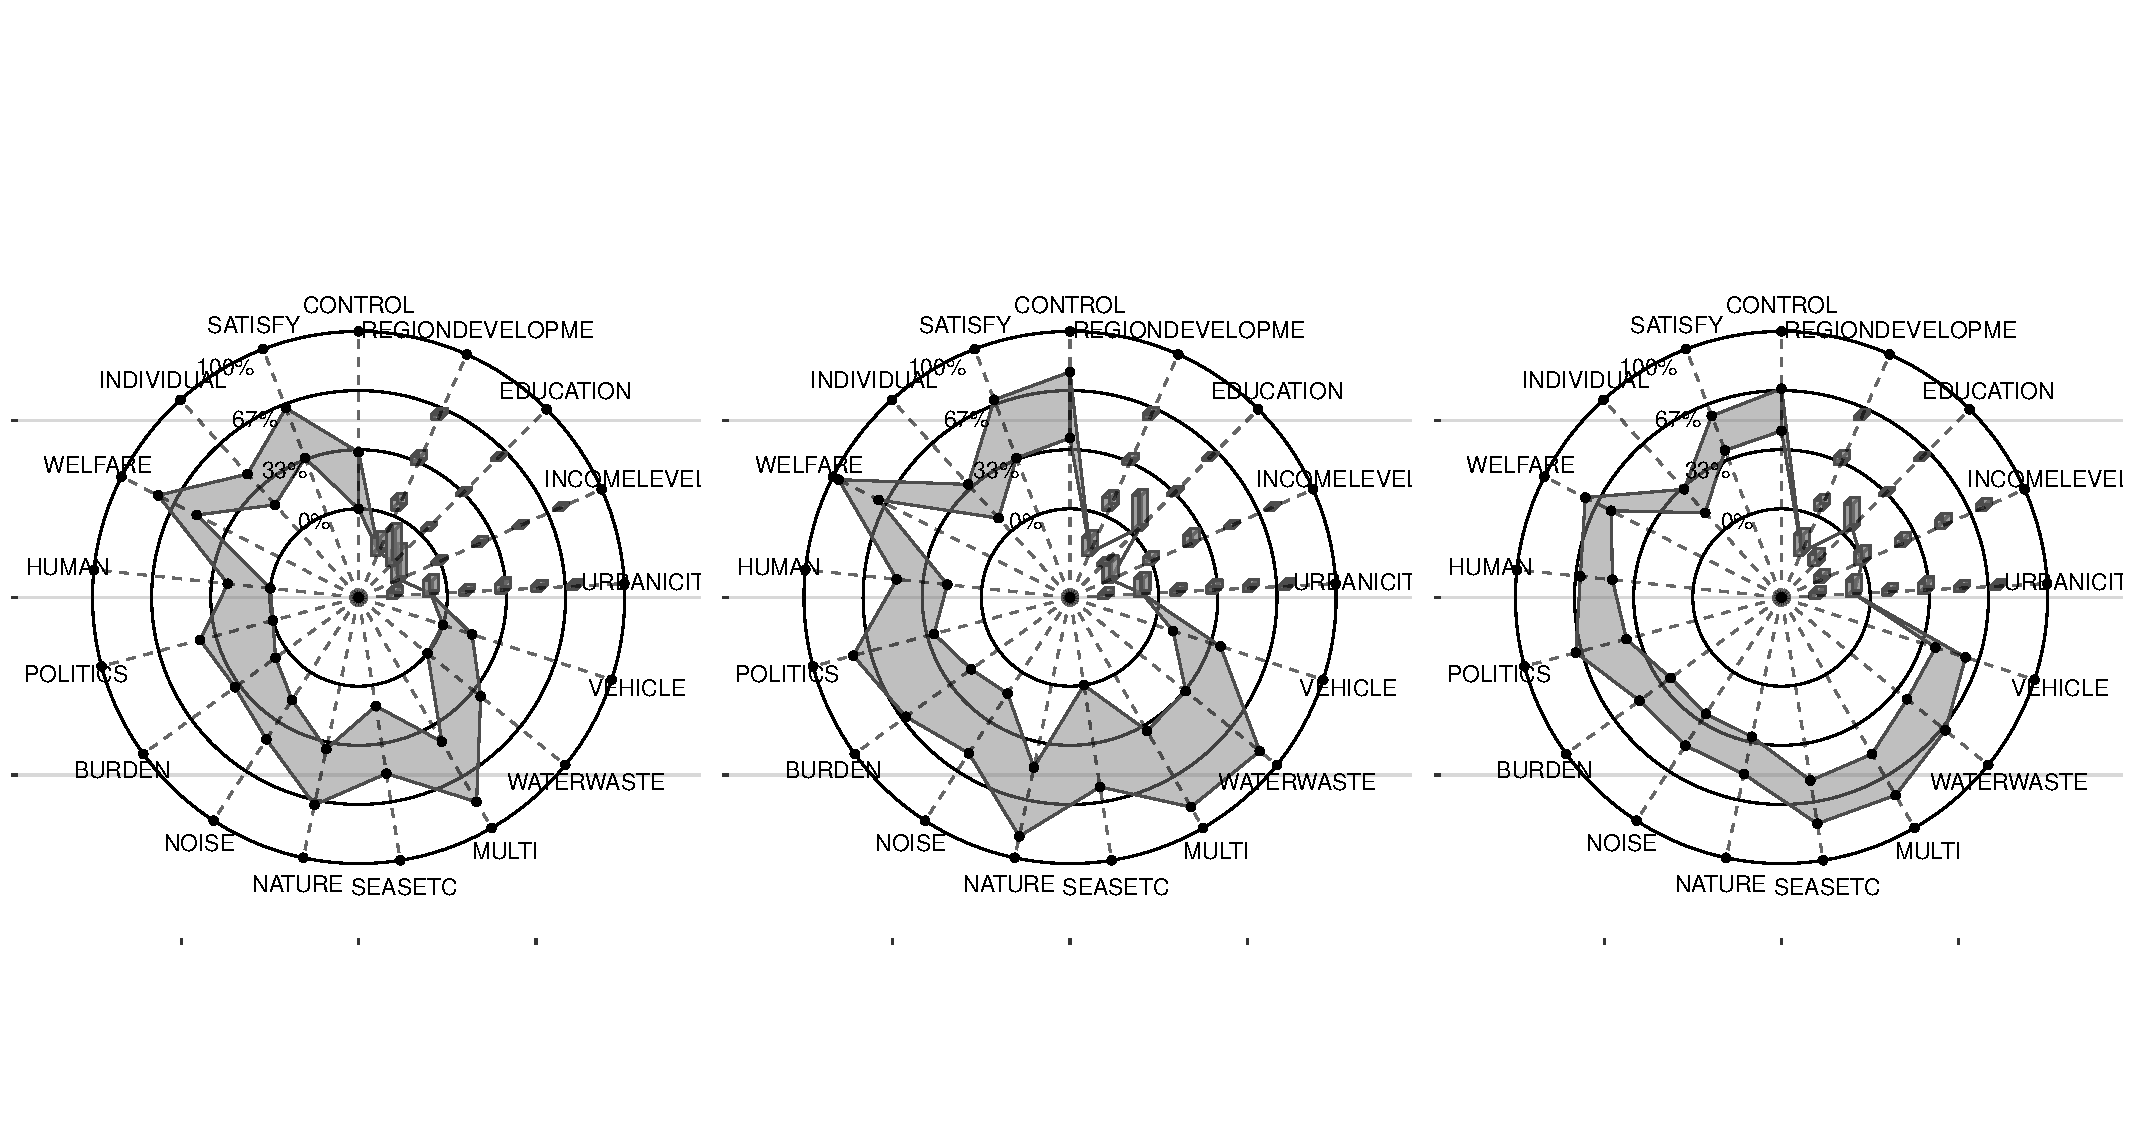
\includegraphics[width=1\textwidth]{pic/radar_3obs} 
\caption{\label{fig:radar_3obs} Compare three distinct observations by multiple variables.}
\end{figure}



%%%%%%%%%%%%%%%%%%%%%%%%%%%
% Figure                  %
%%%%%%%%%%%%%%%%%%%%%%%%%%%
\begin{figure}[t!]
\centering
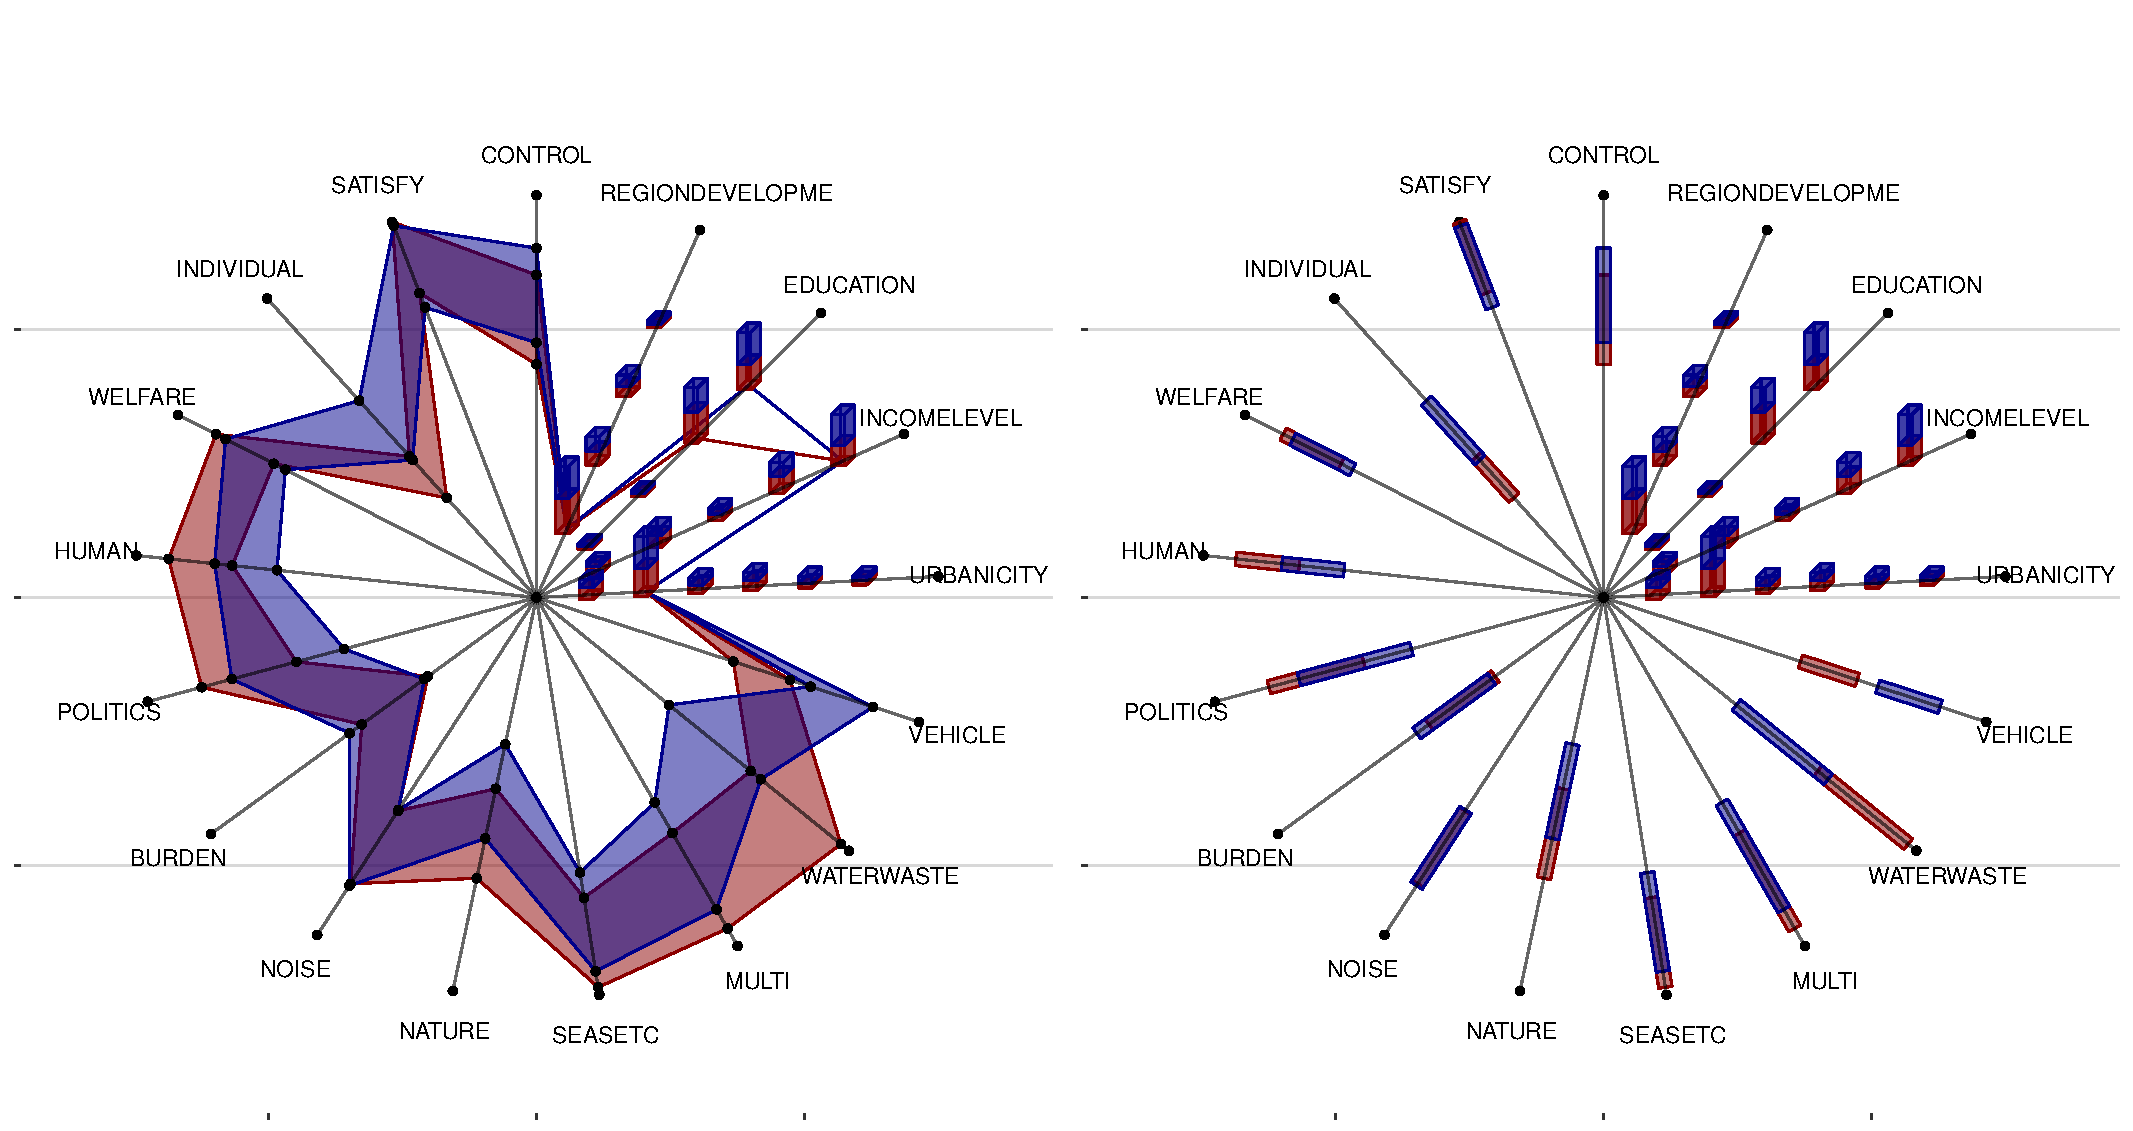
\includegraphics[width=1\textwidth]{pic/radar} 
\caption{\label{fig:radar}  Compare the distinct observations in the same figure by color mapping.}
\end{figure}



%%%%%%%%%%%%%%%%%%%%%%%%%%%
% Figure                  %
%%%%%%%%%%%%%%%%%%%%%%%%%%%
\begin{figure}[t!]
\centering
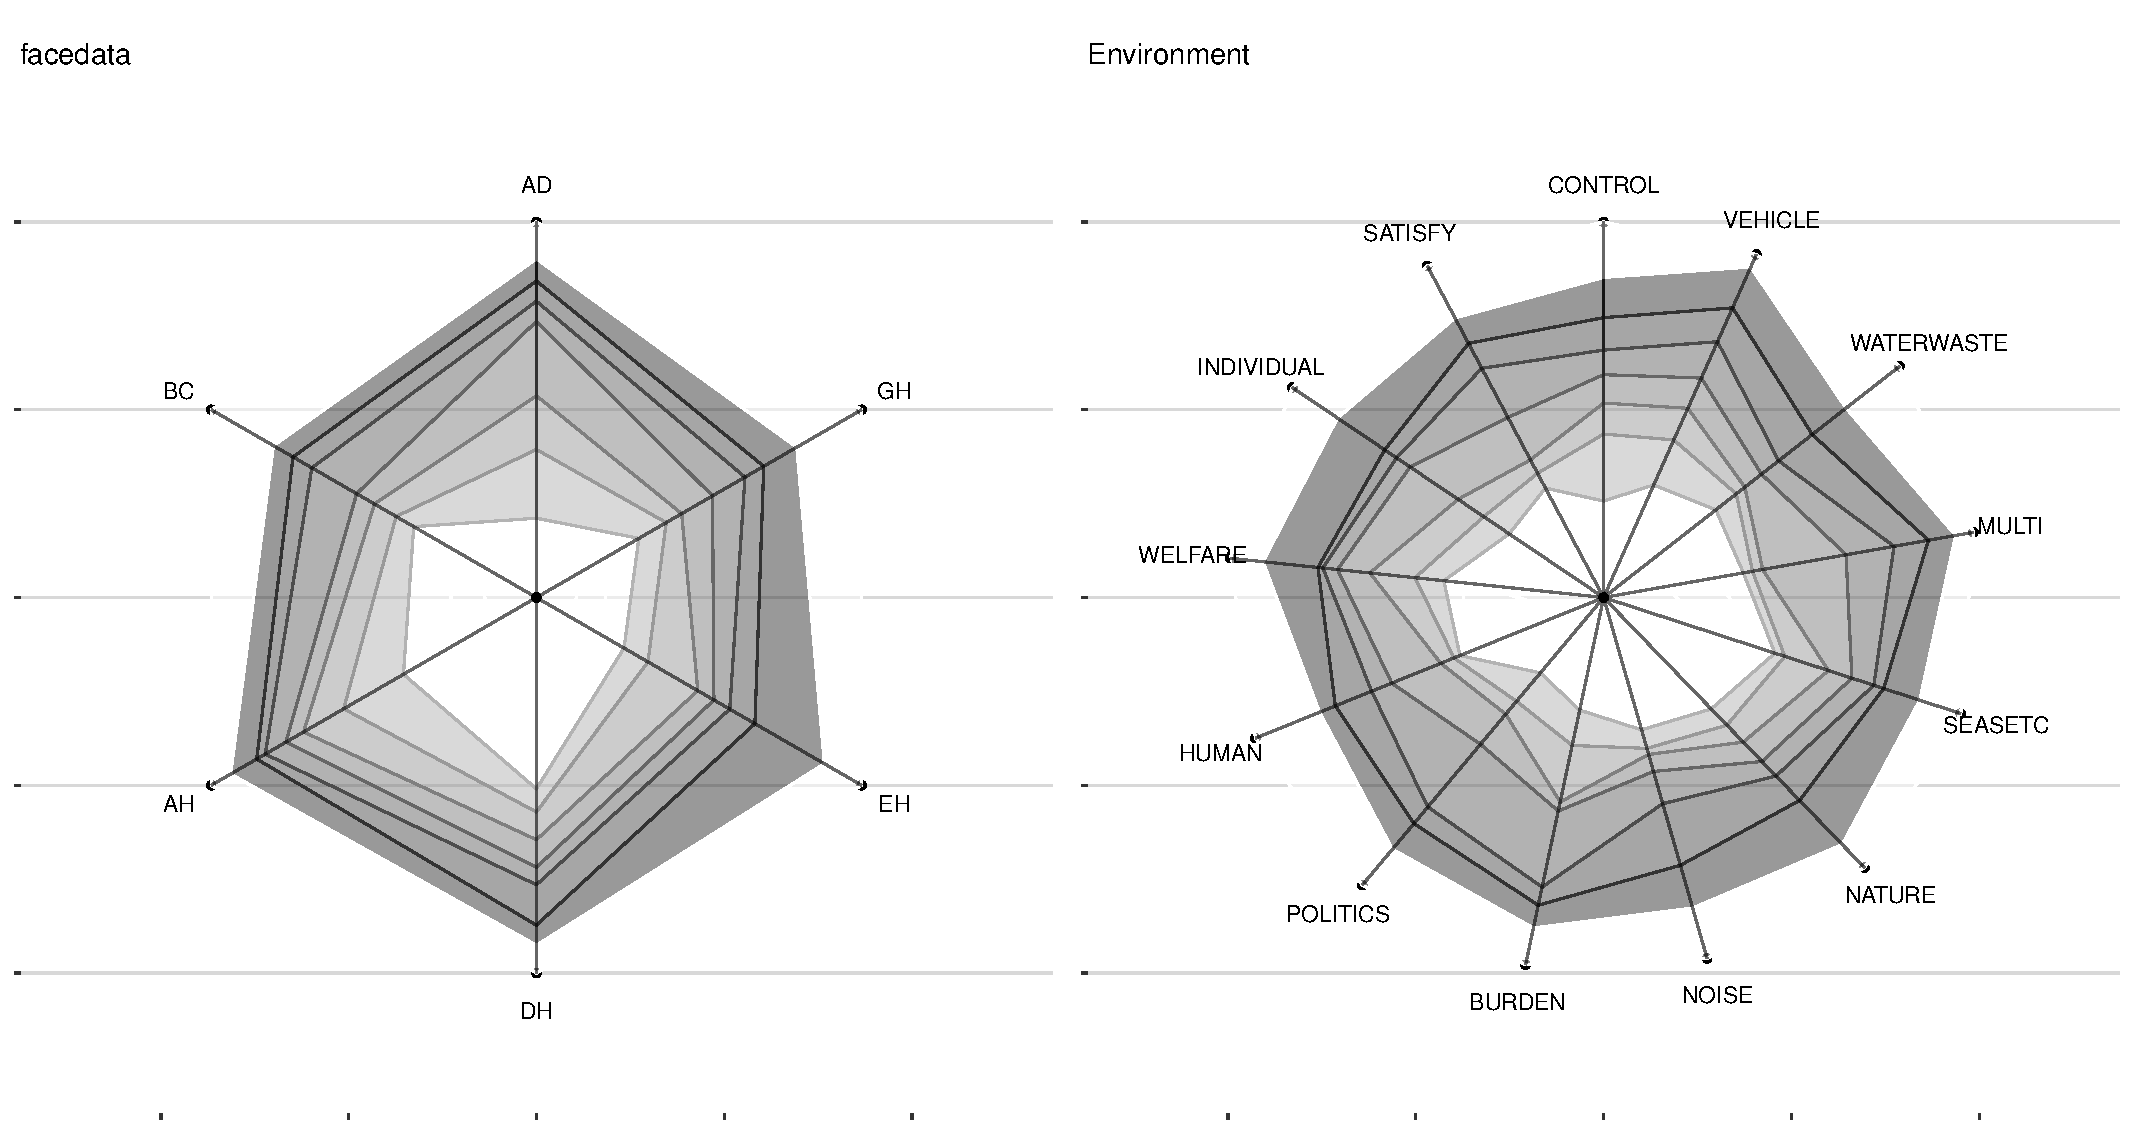
\includegraphics[width=1\textwidth]{pic/radar_2datasets} 
\caption{\label{fig:quantile2} Quantile for two symbolic datasets.}
\end{figure}



%%%%%%%%%%%%%%%%%%%%%%%%%%%
% Figure                  %
%%%%%%%%%%%%%%%%%%%%%%%%%%%
\begin{figure}[t!]
\centering
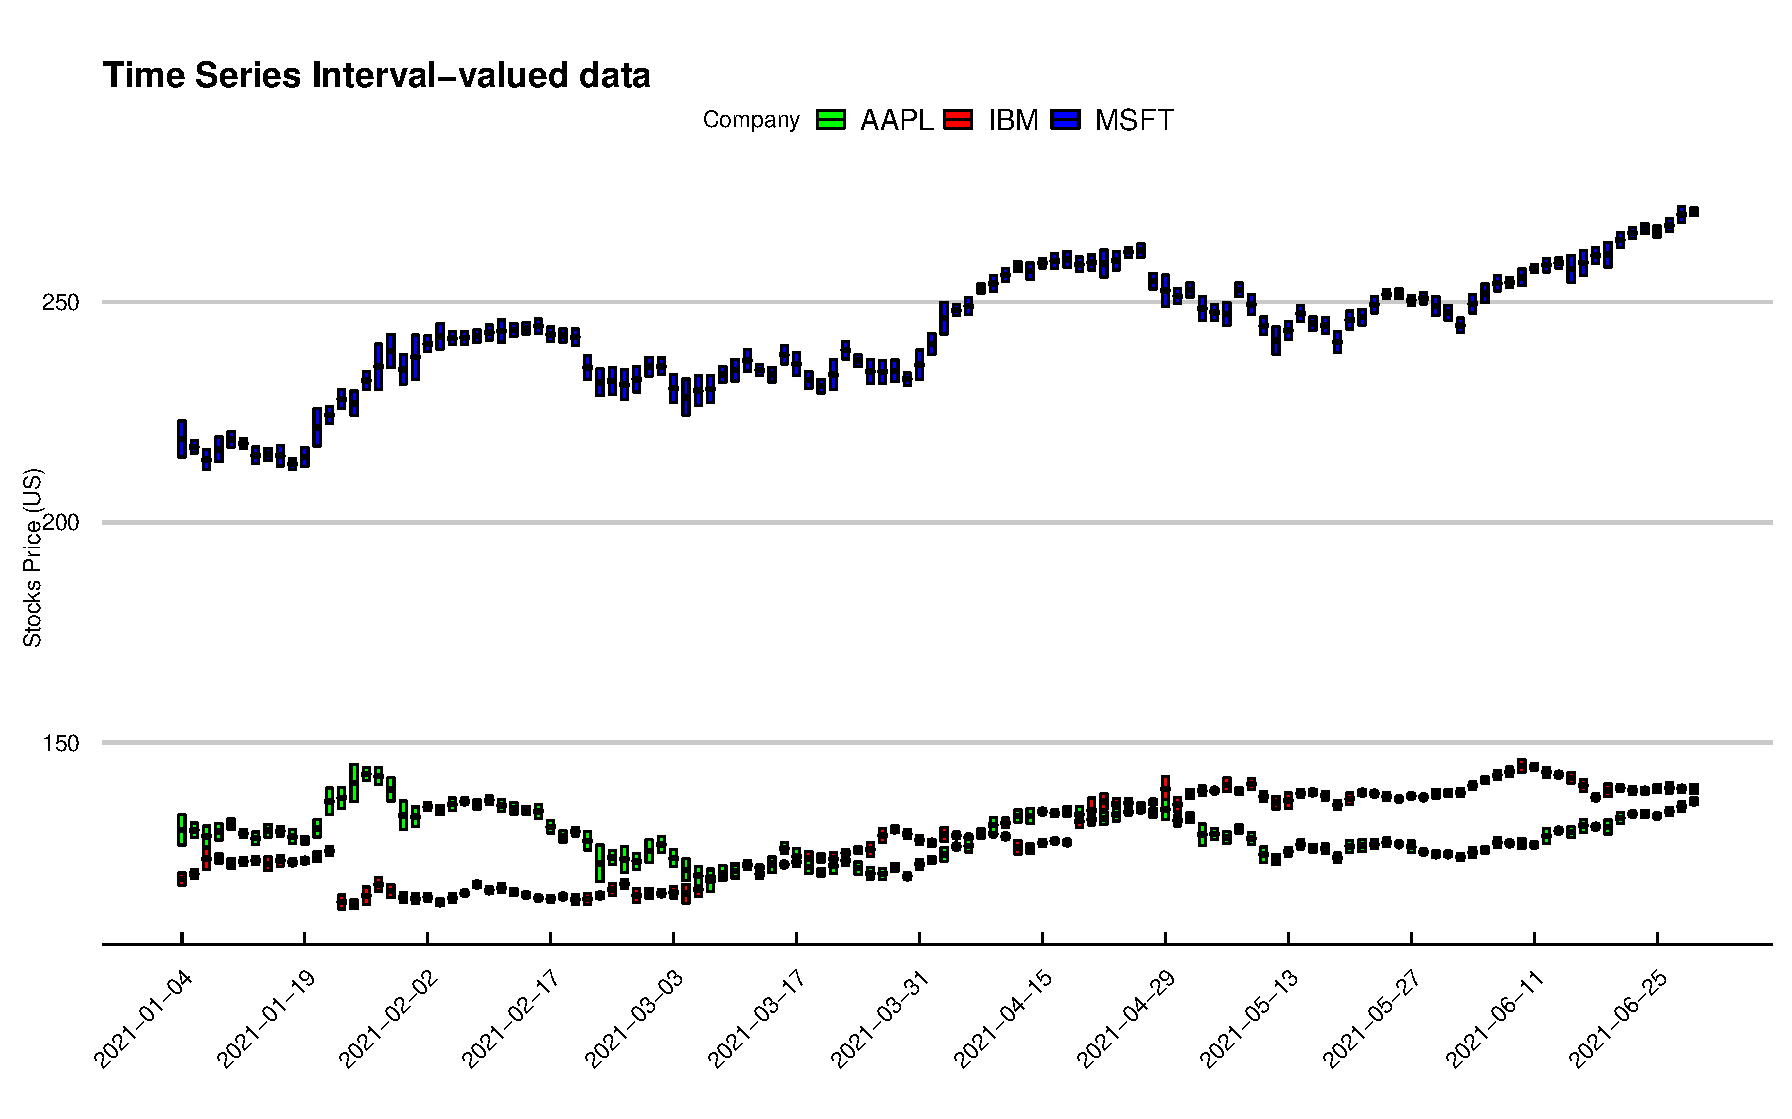
\includegraphics[width=1\textwidth]{pic/ts_3company} 
\caption{\label{fig:ts}}
\end{figure}


%%%%%%%%%%%%%%%%%%%%%%%%%%%
% Figure                  %
%%%%%%%%%%%%%%%%%%%%%%%%%%%
\begin{figure}[t!]
\centering
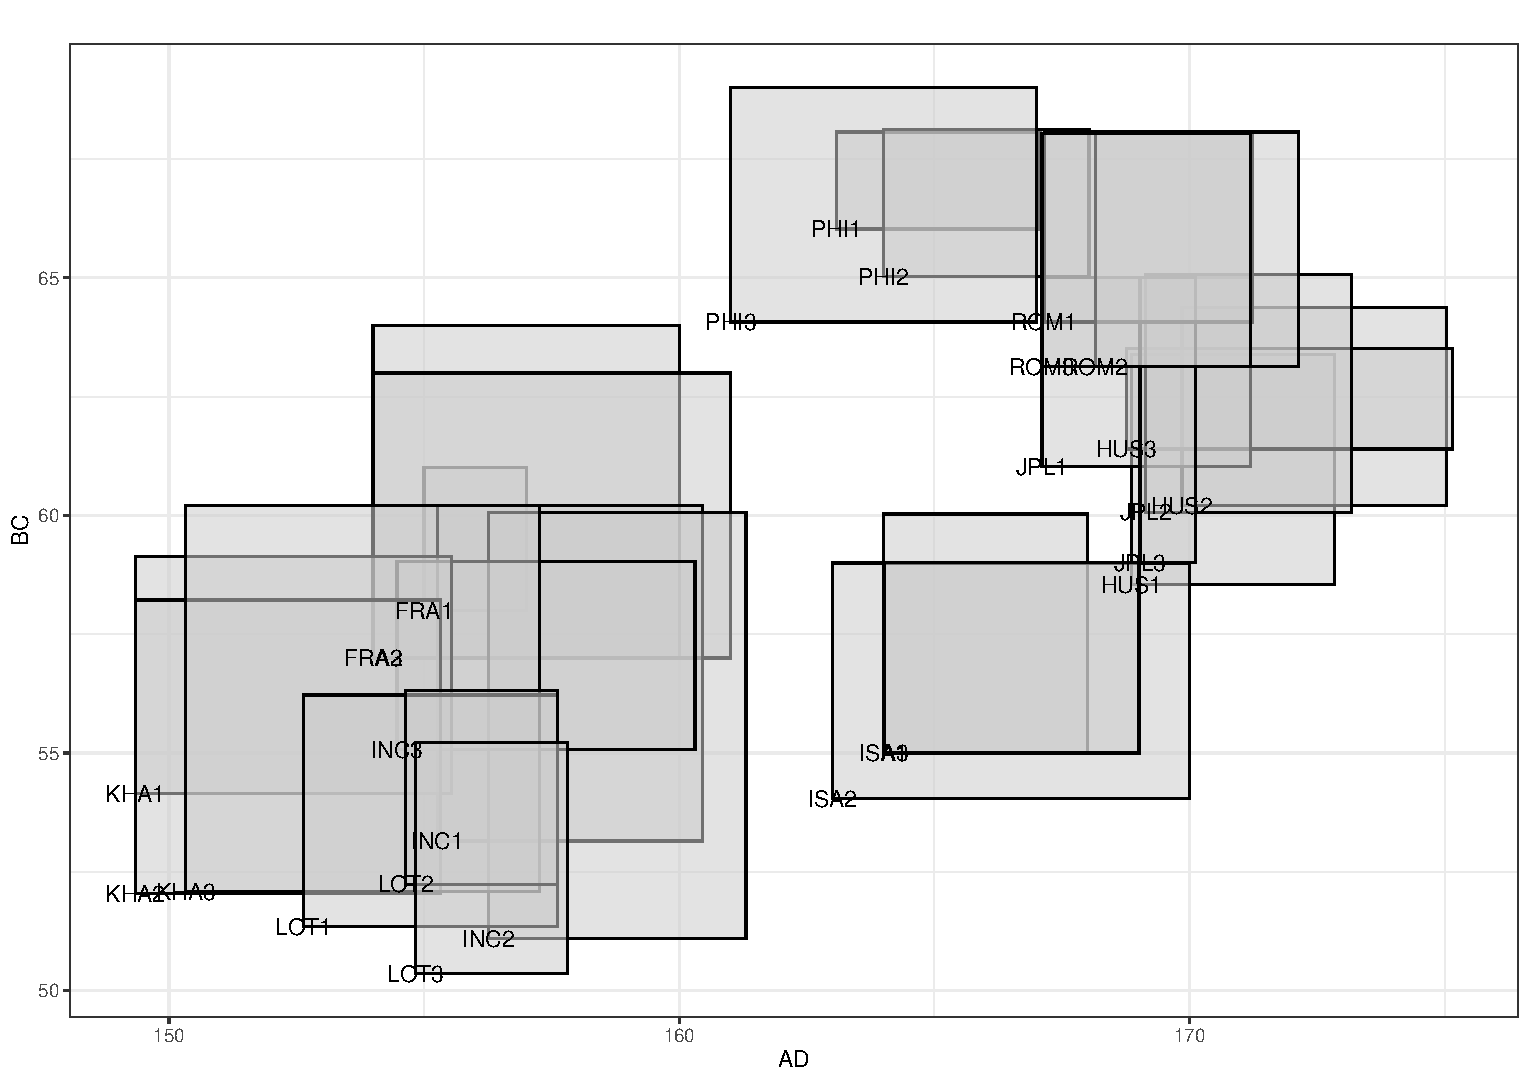
\includegraphics[width=1\textwidth]{pic/scatter} 
\caption{\label{fig:scatter}}
\end{figure}


%%%%%%%%%%%%%%%%%%%%%%%%%%%
% Figure                  %
%%%%%%%%%%%%%%%%%%%%%%%%%%%
\begin{figure}[t!]
\centering
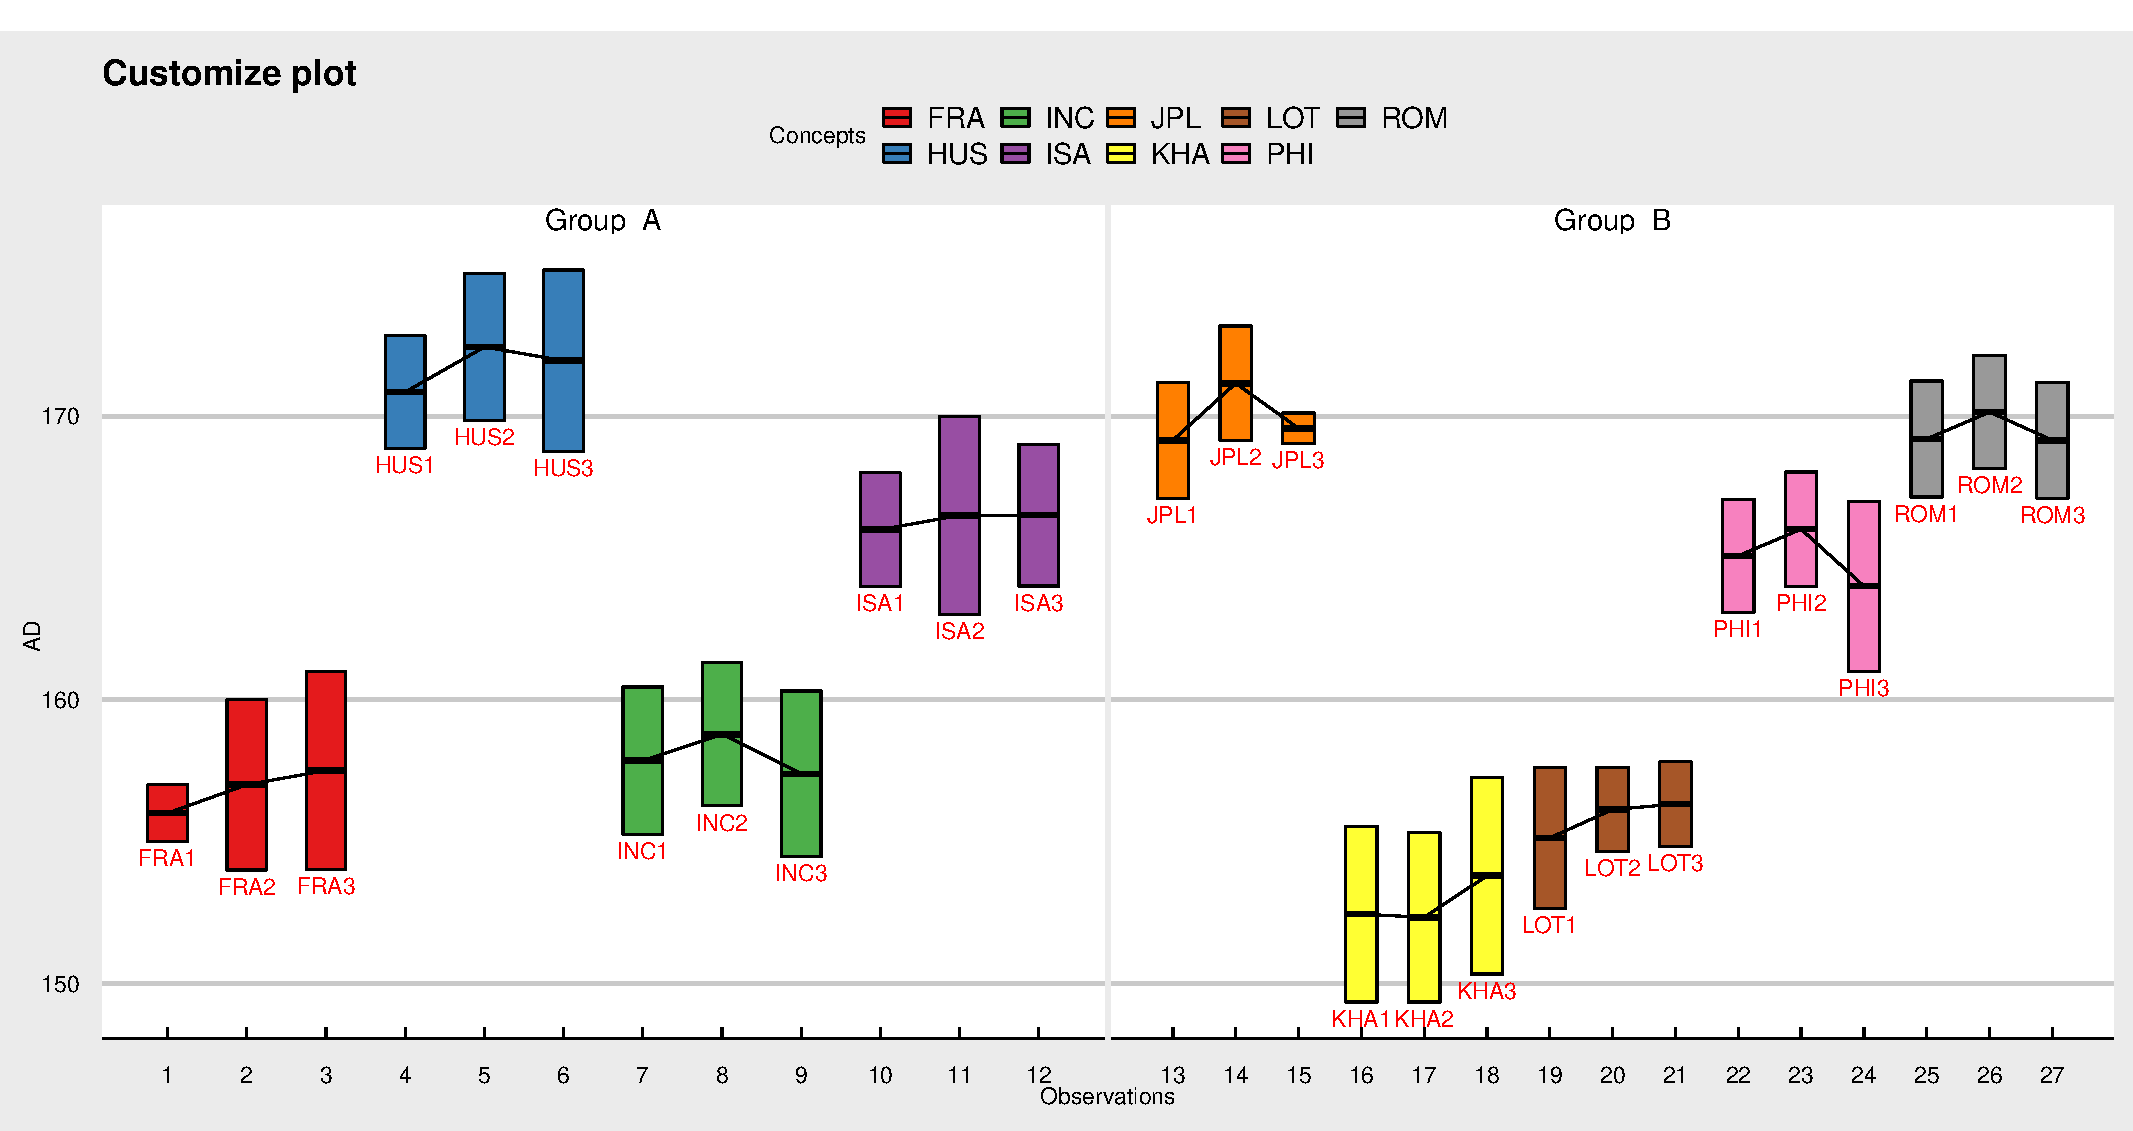
\includegraphics[width=1\textwidth]{pic/customize} 
\caption{\label{fig:customize}}
\end{figure}



%%%%%%%%%%%%%%%%%%%%%%%%%%%
% Figure                  %
%%%%%%%%%%%%%%%%%%%%%%%%%%%
\begin{figure}[t!]
	\centering
	\begin{tabular}{cc}
		(a) & (b) \\ 
		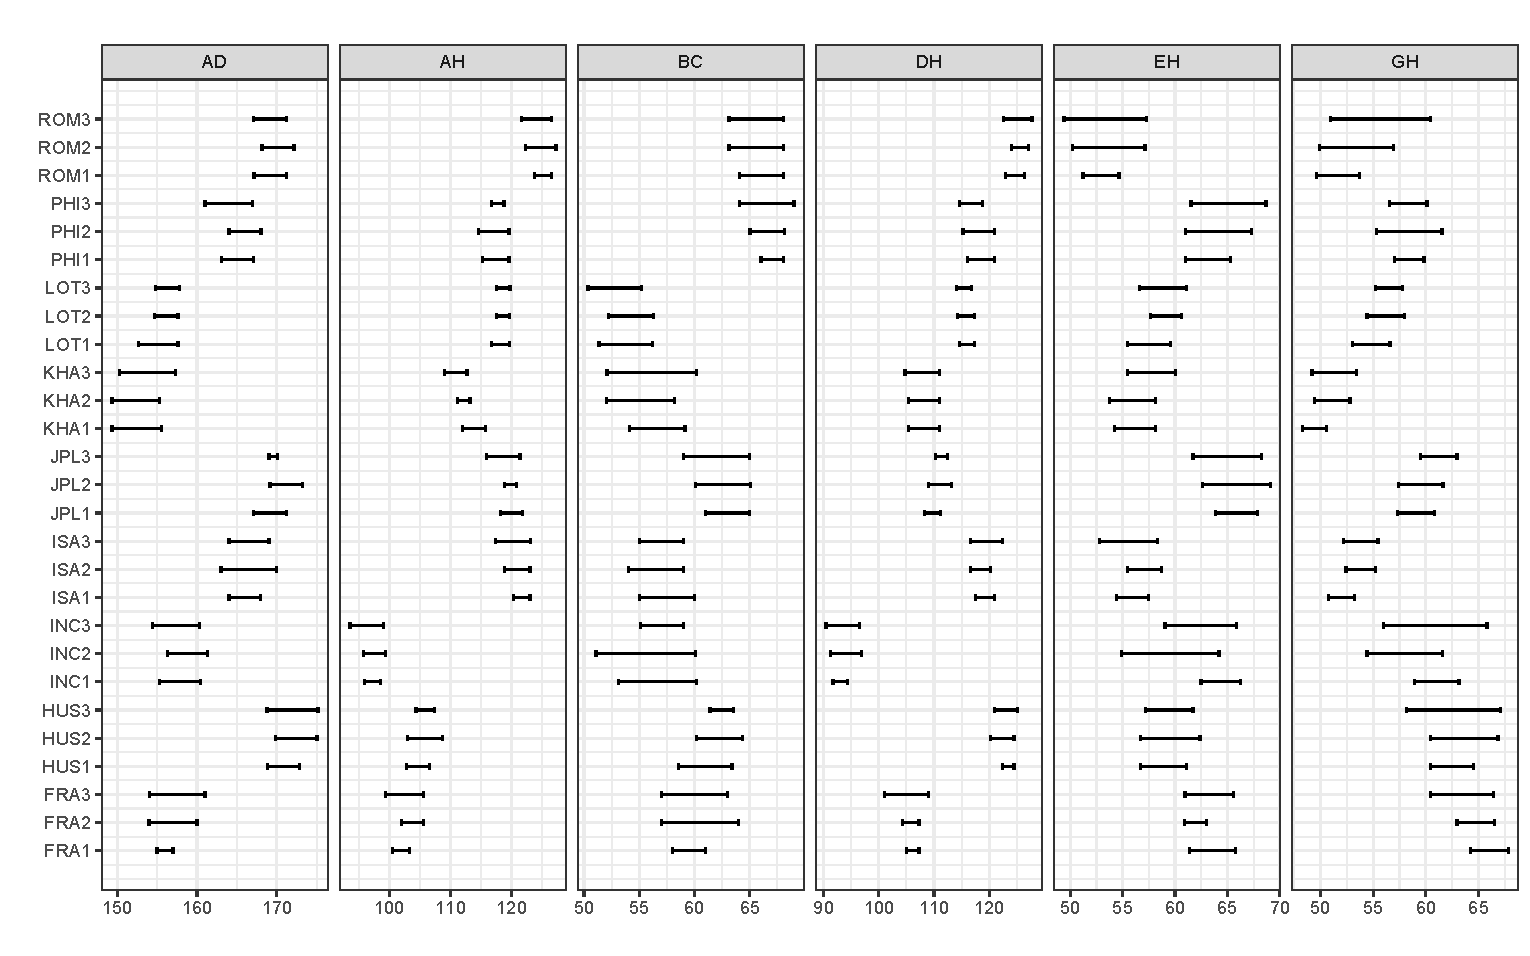
\includegraphics[width=0.5\textwidth]{pic/index_allvar_origin} &
		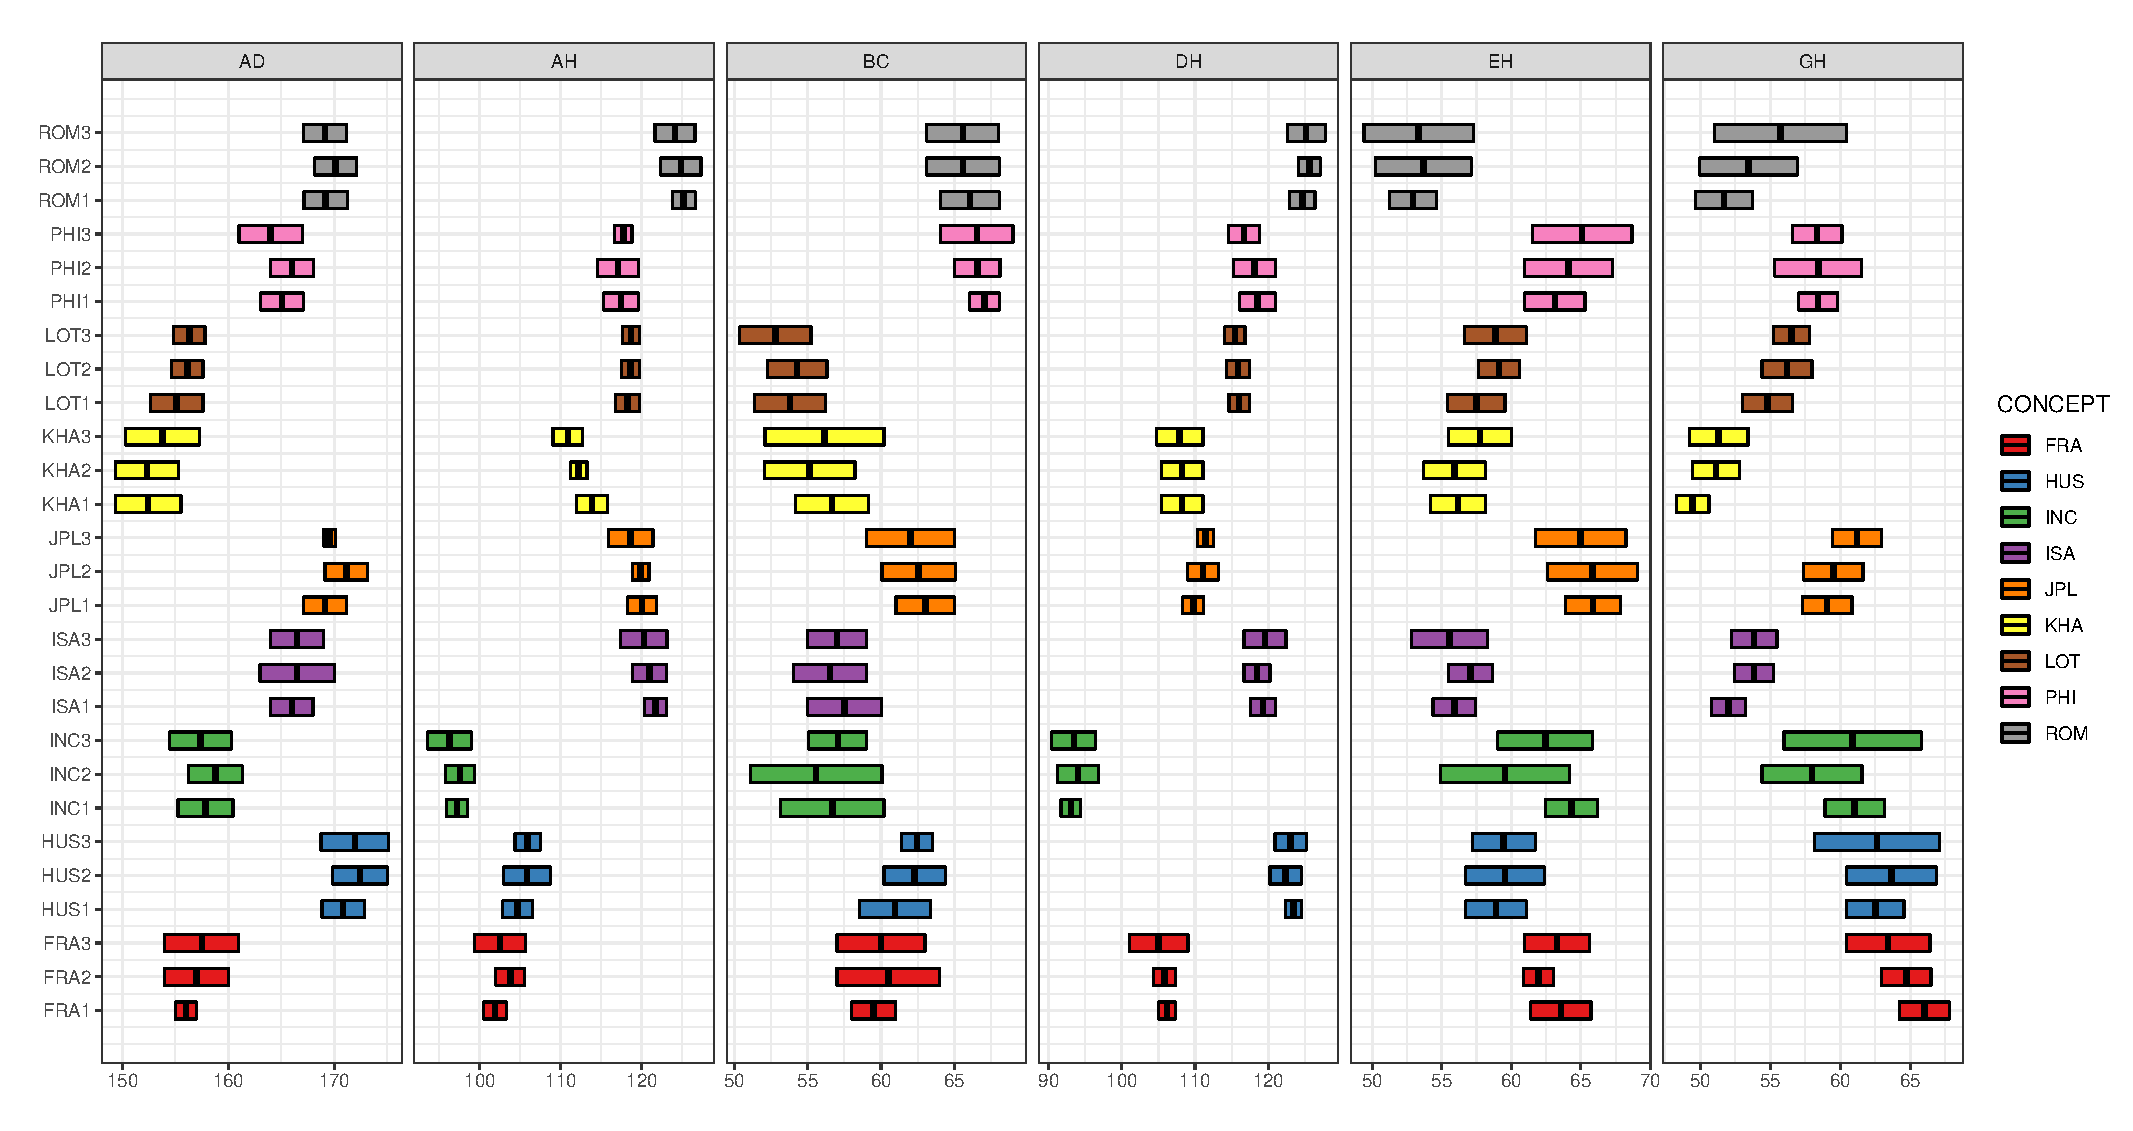
\includegraphics[width=0.5\textwidth]{pic/index_allvar} \\ 
		(c) & (d) \\
		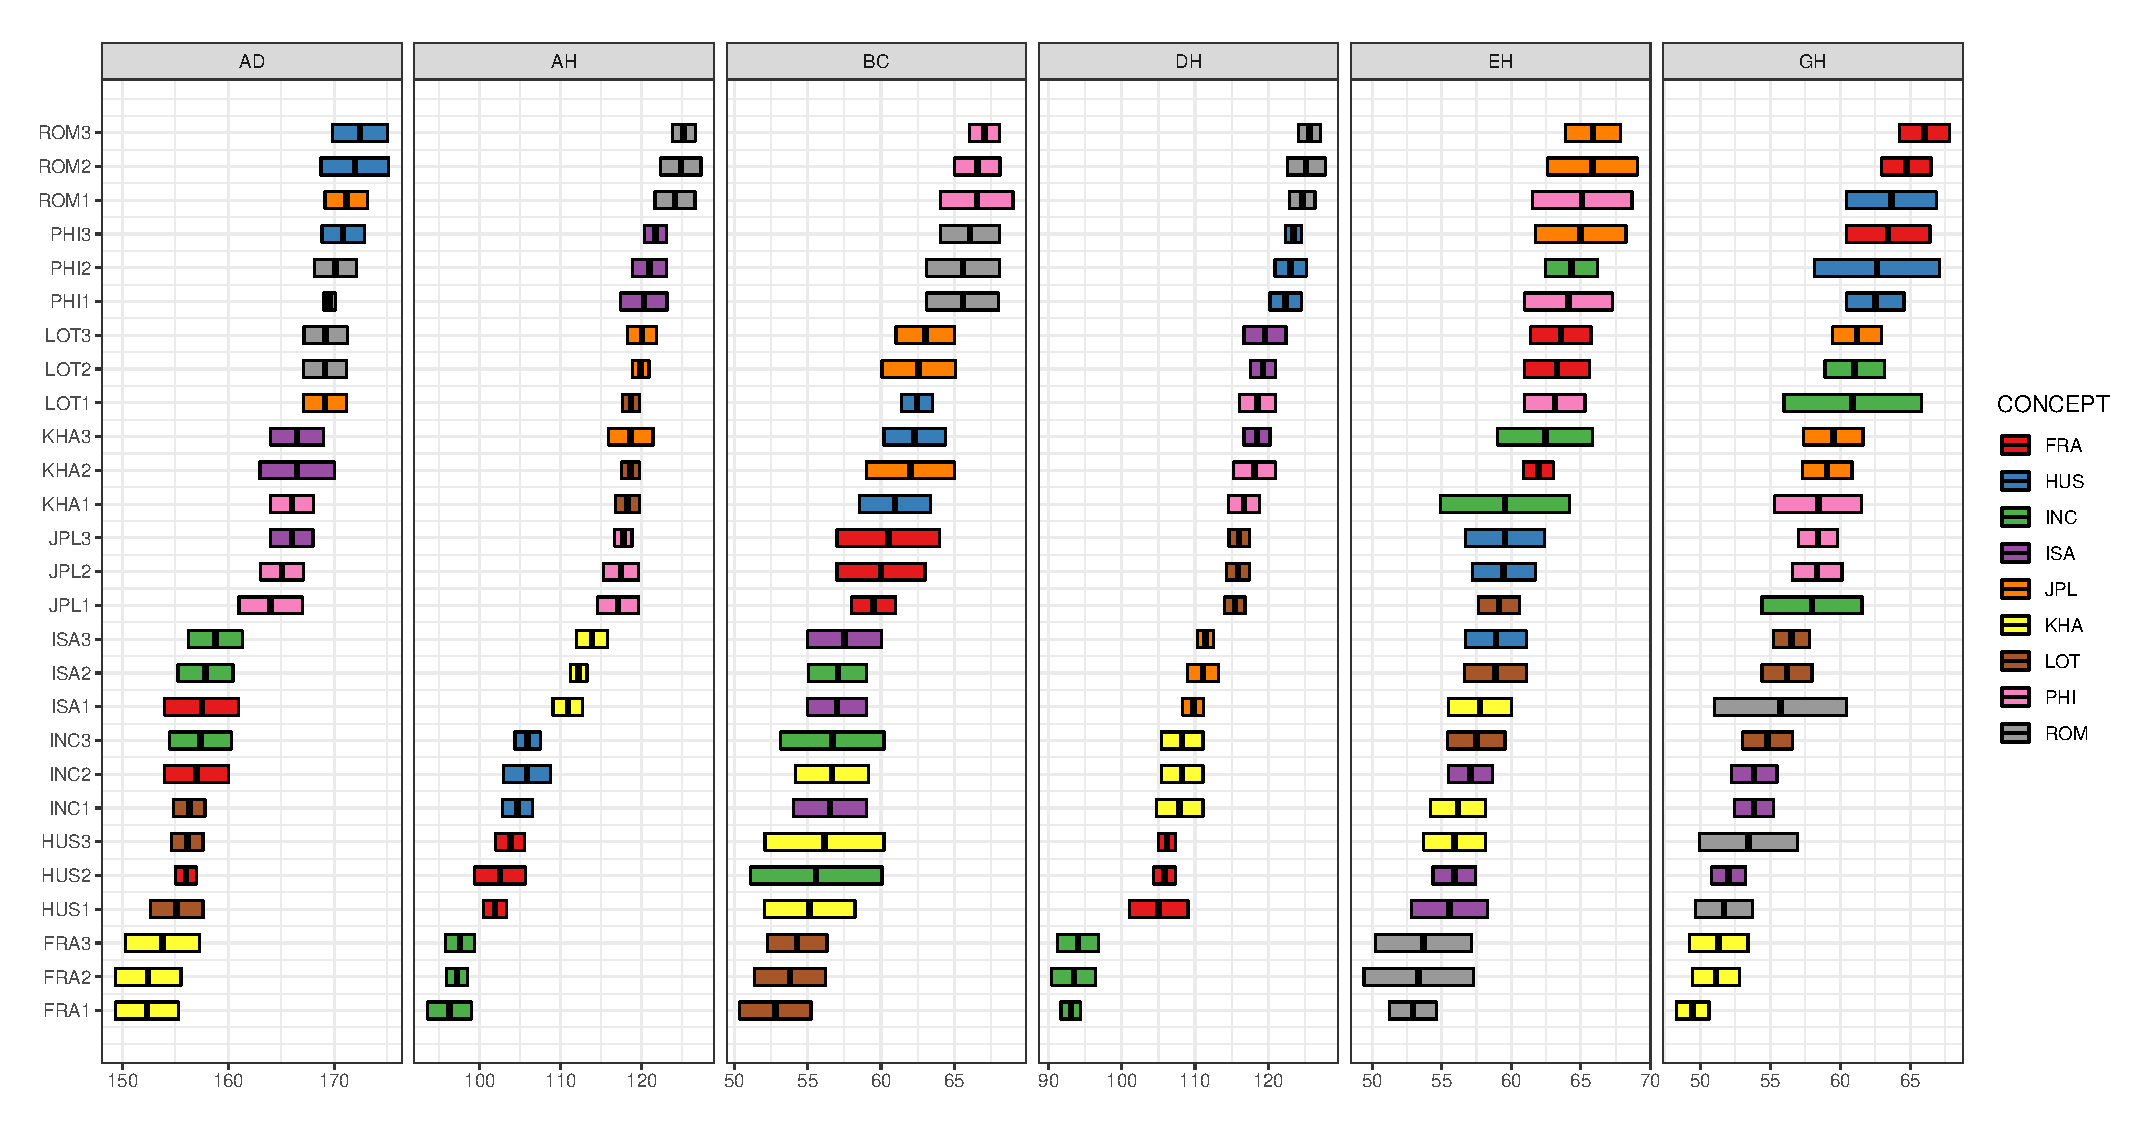
\includegraphics[width=0.5\textwidth]{pic/index_allvar_sort_c} &
		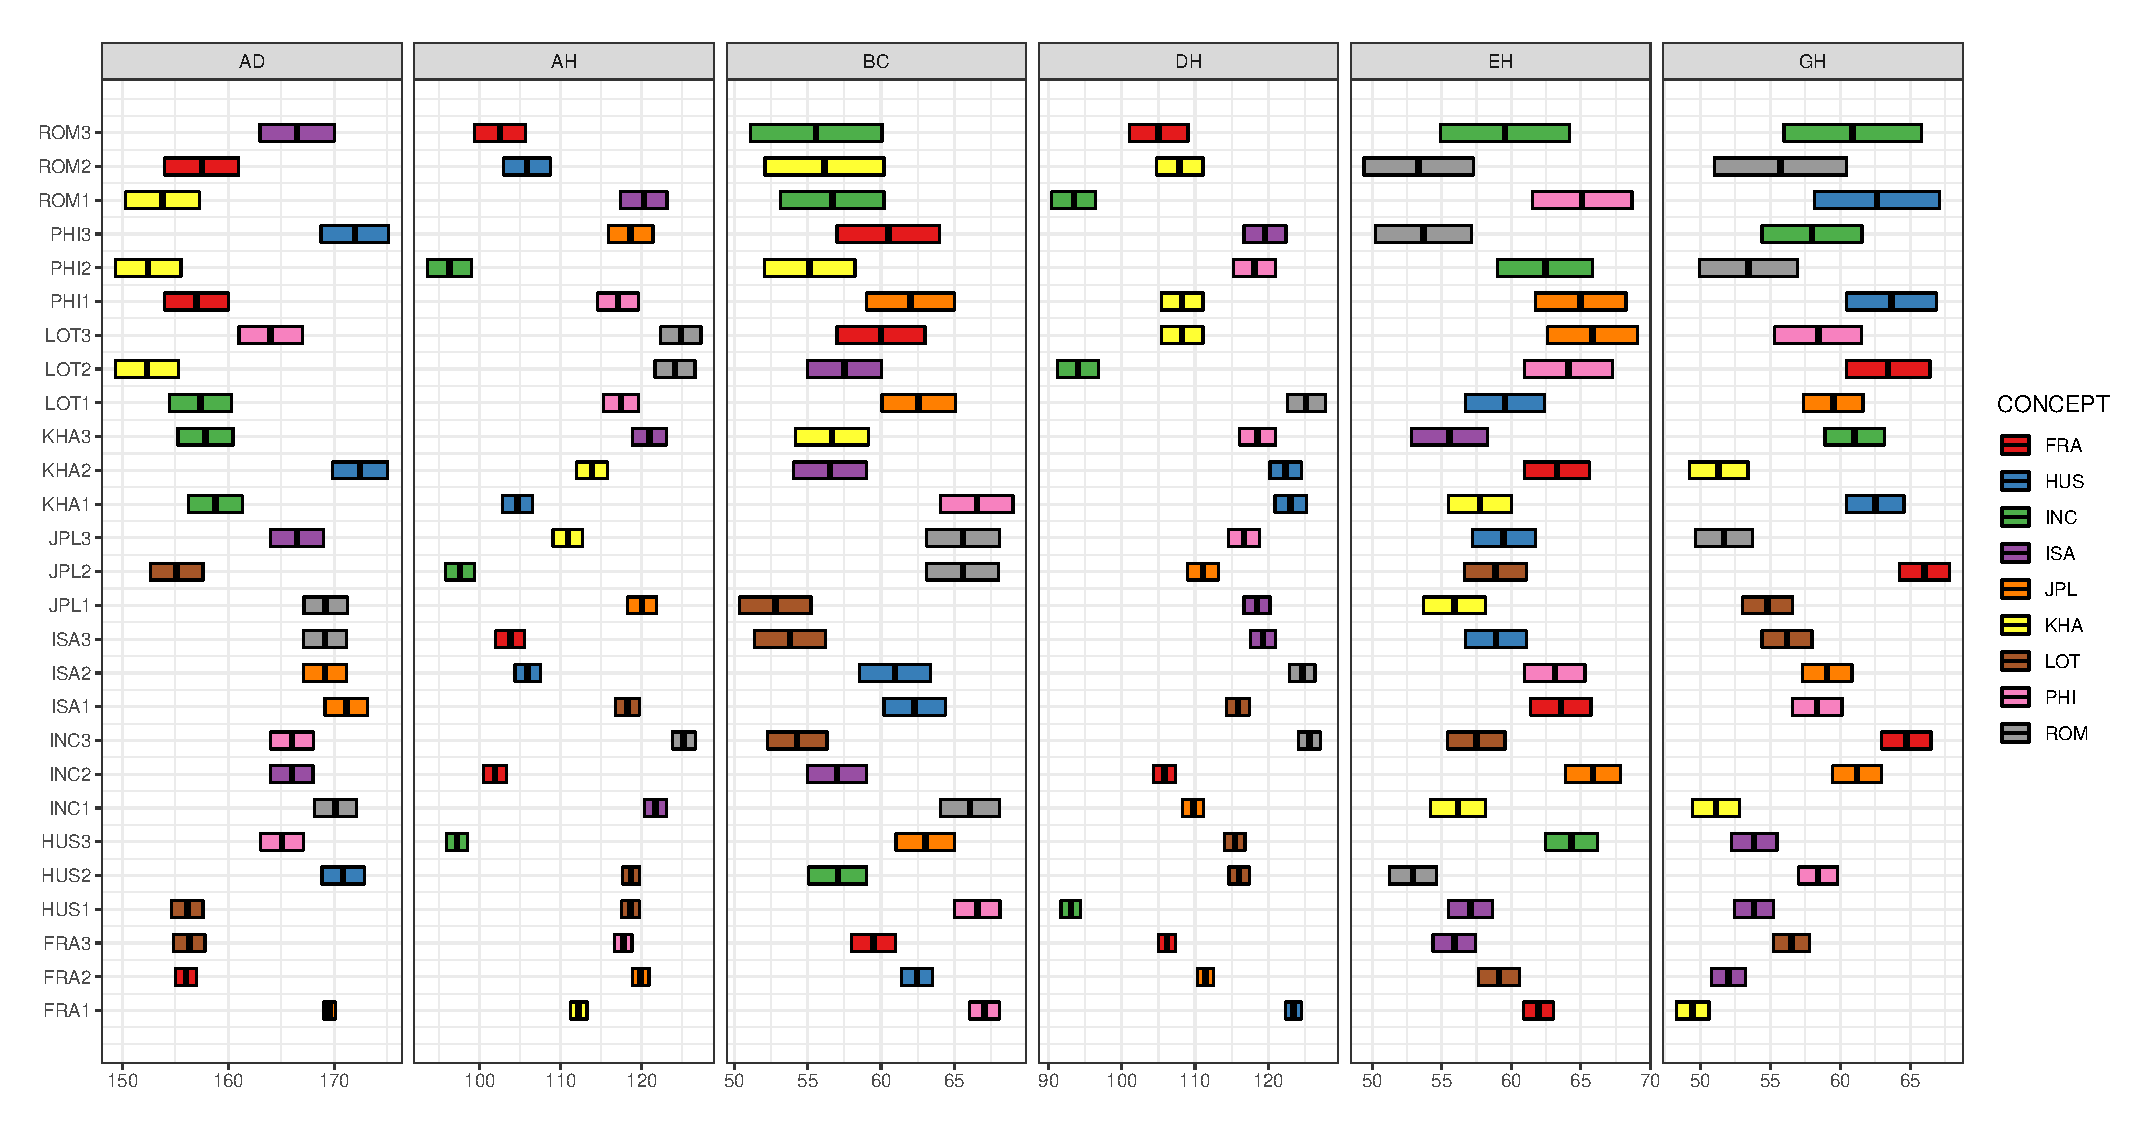
\includegraphics[width=0.5\textwidth]{pic/index_allvar_sort_r} 
	\end{tabular}
	\caption{\label{fig:index_allvar} }
\end{figure}


\end{appendix}

\end{document}
%%%%%%%%%%%%%%%%%%%%%%%%%%%%%%%%%%%%%%%%%%%%%%%%%%%%%%%%%%%%%%%%%%%%%%%%%%%%%%%%
%% END                                                                        %%
%%                                                                            %%
%%                                                                            %%
%%%%%%%%%%%%%%%%%%%%%%%%%%%%%%%%%%%%%%%%%%%%%%%%%%%%%%%%%%%%%%%%%%%%%%%%%%%%%%%%




\iffalse
<<dataPrepare, echo=FALSE, results=hide>>=
options(useFancyQuotes=FALSE) #debug for is not ACSII
myLibrary <- c("ggESDA", "data.table", "dplyr")
new.packages <- myLibrary[!(myLibrary %in% installed.packages()[,"Package"])]
if(length(new.packages)) install.packages(new.packages)
lapply(myLibrary, require, character.only = TRUE)

Concepts <- as.factor(rep(c("FRA", "HUS", "INC", "ISA", "JPL", "KHA",
                        "LOT", "PHI", "ROM"), each = 3))

set.seed(20211020)
myDiamonds <- diamonds
myDiamonds.i <- classic2sym(myDiamonds)$intervalData
breastData <- data.table::fread("data/data.csv")


scale_sym_table <- function(d){
  n <- dim(d)[1]
  p <- dim(d)[2]
  temp1 <- sapply(1:p, FUN = function(x) unlist(data.frame(d[[x]])))
  temp2 <- apply(temp1, 2, scale)
  newd <- data.frame(temp2[1:n, ], temp2[(n+1):(n*2), ])
  myd <- classic2sym(newd, groupby = "customize",
                     minData = temp2[1:n, ],
                     maxData = temp2[(n+1):(n*2), ])
  colnames(myd$intervalData) <- colnames(d)
  return(myd$intervalData)
}

this.data <- facedata
@
\fi



\\
%%%%%%%%%%%%%%%%%%%%%%%%%%%%%%%%%%
%                                %
%%%%%%%%%%%%%%%%%%%%%%%%%%%%%%%%%%
\subsection{DR for high-dimensional data and big data}
There have been many studies concerned about the (ultra)
high-dimensional data analysis in the communities of
statistics (e.g., Candes and Tao, 2007; Fan and Lv, 2008;
Hall and Miller, 2009) and machine learning (e.g., Bae,
Choi and Qiu, 2010; Niyogi, Smale, and Weinberger, 2011).
Restrict the researches to the dimensionality reduction
only, most of the major methods are based on SVD, PCA, MDS
or ISOMAP (Tenenbaum {\it et al.}, 2000). On the other
hand, the applications of DR to big data were not so common
seen until now. The developed methodologies and
applications of DR is getting more important in the era of
big data (Yoo, Ramirez, Liuzzi, 2014; Feldman, Schmidt,
Sohler, 2013). Gunarathne {\it et al.} (2011) utilized
cloud computing techniques based on the data processing
framework such as Hadoop and MapReduce to perform dimension
reduction in the analysis of chemical structure. Jiang,
Weitz, and Dushoff (2012) developd a dimension reduction
approach based on the non-negative matrix factorization
(NMF) for identifying modular patterns in metagenomic
profile data. Cunningham and Yu (2014) used various
dimensionality reduction methods (both linear and
nonlinear) for analyzing large-scale neural recordings.
Wilkerson, Chintakunta,and Krim, (2014) suggested a
computing algorithm based on a distributed dimension
reduction approach for big data. Wikle, Holan, and Hooten,
(2013) edited a journal special issue on modern dimension
reduction methods for big data problems in ecology. In this
special issue, the DR methods, in a broad sense, concerned
the multivariate or spatiotemporal processes and data. The
objects associated with dimension reduction were either in
terms of the parameters, state-process, or grouping. As
stated by the editors, the challenges with high
dimensionality are further increased by the non-Gaussian
and/or nonlinear nature of the data and processes of
interest.





%%%%%%%%%%%%%%%%%%%%%%%%%%%
% Table                   %
%%%%%%%%%%%%%%%%%%%%%%%%%%%
\begin{table}[t!]
\centering{\scriptsize
\begin{tabular}{|l|l|c|c|ccc|c|c|c|} \hline
\multicolumn{1}{r}{} & \multicolumn{1}{r}{} & \multicolumn{1}{c}{\textbf{ Available}} & \multicolumn{1}{c}{\textbf{Summarize}} & \multicolumn{3}{c}{\textbf{EDA}} & \multicolumn{1}{c}{\textbf{Statistic}} & \multicolumn{2}{c}{\textbf{Machine learning}} \\ \hline
\multicolumn{1}{c|}{Package} & \multicolumn{1}{c|}{Author} & Version & Function & Univariate & Bivariate & Multivariate & Stat. Method & Supervised & \multicolumn{1}{c}{Unsupervised} \\ \hline
RSDA  & Rojas et al. (2015) & R(4.1.0)     & \code{classic.to.sym}     & -     & 1     & -     & 3     & \textbf{2}    & \textbf{1} \\
symbolicDA & Dudek et al. (2013) & R(4.1.0)     &    -   & -     & -     & \textbf{2}    & 2     & 1     & \textbf{1} \\
HistDAWass & Irpino (2015) & R(4.1.0)     & \code{data2hist}     & 4     & -     & -     & 3     & 1     & \textbf{1} \\    
MAINT.Data & Silva \&  Brito (2011) & R(4.1.0)     &   -    & -     & -     & -     & \textbf{7}    & -     & \textbf{1} \\ \hline
iRegression & Neto et al. (2011) & R(4.1.0)     &   -    & -     & -     & -     & 1     & -     & - \\
intReg & Toomet (2012) & R(3.6.0)      &  -     & -     & -     & -     & 1     & -     & - \\
ISDA.R & Filho \&  Fagundes (2012) & R(2.15.2)      &    -   & 1     & -     & 1     & 1     & -     & - \\
GPCSIV & Brahim (2013) & R(3.0.2)      &  -     & -    & -     & -     & 1     & -     & - \\
GraphPCA & Brahim \& Kallyth (2014) & R(4.1.0)      &   -    & -     & 1     & 1     & 1     & -     & - \\ \hline
ggESDA & Jiang (2021) & R(4.1.0)     & \code{classic2sym}     & \textbf{8}    & \textbf{4}    & \textbf{2}    & 1     & -     & - \\ \hline
\end{tabular}}%
\caption{\label{tab:pkgCompare} Compare with \proglang{R} packages.}
\end{table}%


As stated by \cite{Diday:2018} "In Data Science the aim is to extract
new knowledge from Standard, Big, and complex data. Often these data
are unstructured with variables defined on different kinds of units.
They can also be multi-sources (as mixtures of numerical and textual
data, with images and networks)." It indicates that not only
conventional data but the unstructured data, also known as symbolic
data, is vital for data science. Rather than the classical data
represented by a single value, symbolic data with measurements on $p$
random variables can be $p$-dimensional statistical units such as
hypercubes or histograms. 

The field of symbolic data analysis (SDA)
\cite{Billard+Diday:2007} is to broaden the application aspects of
statistical methodologies, extend traditional cognition of a form of
data unit and build a brand-new analysis system of data science.
Recent developments in the field of big data analytics have led to a
renewed interest in complex structure data such as symbolic data. 



%% Completeness of information
To lead researchers to explore more details in what they are
interesting such as a particular part of data, aggregation methods
play a vital role to merge the data we interesting. However, the
conventional data after merging will usually be represented by a
single value (especially mode or mean), which will be unmeaningful to
visualize and cause the loss of information that may become larger
when the data or the number of factors in that category is growing on.
For the category data, SDA will build a histogram by calculating each
factor of the category of frequency as bins to solve this kind of
problem as a result. In the way, a categorical variable will never be
shown as a single value at all, instead, a complete information
histogram will be substituted.



The preliminary analysis of data to discover relationships between
measures in the data and to gain an insight on the trends, patterns,
and relationships among various entities present in the data set with
the help of statistics and visualization tools is called Exploratory
Data Analysis (EDA).


%%%% ggplot() + geom_I()...  vs  ggInterval() + ...
% 格式1 ggplot() + geom_I() + stat_I()...
% 格式2 ggInterval_*() + geom() + stat()...




"Specifically, ggplot2 makes no consideration on what is required for a particular geometry to remain valid within a potentially higher-dimensional coordinate system"





